\documentclass[12pt,]{krantz}
\usepackage{lmodern}
\usepackage{amssymb,amsmath}
\usepackage{ifxetex,ifluatex}
\usepackage{fixltx2e} % provides \textsubscript
\ifnum 0\ifxetex 1\fi\ifluatex 1\fi=0 % if pdftex
  \usepackage[T1]{fontenc}
  \usepackage[utf8]{inputenc}
\else % if luatex or xelatex
  \ifxetex
    \usepackage{mathspec}
  \else
    \usepackage{fontspec}
  \fi
  \defaultfontfeatures{Ligatures=TeX,Scale=MatchLowercase}
\fi
% use upquote if available, for straight quotes in verbatim environments
\IfFileExists{upquote.sty}{\usepackage{upquote}}{}
% use microtype if available
\IfFileExists{microtype.sty}{%
\usepackage{microtype}
\UseMicrotypeSet[protrusion]{basicmath} % disable protrusion for tt fonts
}{}
\usepackage[margin=1in]{geometry}
\usepackage{hyperref}
\PassOptionsToPackage{usenames,dvipsnames}{color} % color is loaded by hyperref
\hypersetup{unicode=true,
            pdftitle={R을 사용한 비구획분석},
            pdfauthor={배균섭, 한성필, 윤석규, 조용순},
            colorlinks=true,
            linkcolor=Maroon,
            citecolor=Blue,
            urlcolor=Blue,
            breaklinks=true}
\urlstyle{same}  % don't use monospace font for urls
\usepackage{color}
\usepackage{fancyvrb}
\newcommand{\VerbBar}{|}
\newcommand{\VERB}{\Verb[commandchars=\\\{\}]}
\DefineVerbatimEnvironment{Highlighting}{Verbatim}{commandchars=\\\{\}}
% Add ',fontsize=\small' for more characters per line
\usepackage{framed}
\definecolor{shadecolor}{RGB}{248,248,248}
\newenvironment{Shaded}{\begin{snugshade}}{\end{snugshade}}
\newcommand{\KeywordTok}[1]{\textcolor[rgb]{0.13,0.29,0.53}{\textbf{#1}}}
\newcommand{\DataTypeTok}[1]{\textcolor[rgb]{0.13,0.29,0.53}{#1}}
\newcommand{\DecValTok}[1]{\textcolor[rgb]{0.00,0.00,0.81}{#1}}
\newcommand{\BaseNTok}[1]{\textcolor[rgb]{0.00,0.00,0.81}{#1}}
\newcommand{\FloatTok}[1]{\textcolor[rgb]{0.00,0.00,0.81}{#1}}
\newcommand{\ConstantTok}[1]{\textcolor[rgb]{0.00,0.00,0.00}{#1}}
\newcommand{\CharTok}[1]{\textcolor[rgb]{0.31,0.60,0.02}{#1}}
\newcommand{\SpecialCharTok}[1]{\textcolor[rgb]{0.00,0.00,0.00}{#1}}
\newcommand{\StringTok}[1]{\textcolor[rgb]{0.31,0.60,0.02}{#1}}
\newcommand{\VerbatimStringTok}[1]{\textcolor[rgb]{0.31,0.60,0.02}{#1}}
\newcommand{\SpecialStringTok}[1]{\textcolor[rgb]{0.31,0.60,0.02}{#1}}
\newcommand{\ImportTok}[1]{#1}
\newcommand{\CommentTok}[1]{\textcolor[rgb]{0.56,0.35,0.01}{\textit{#1}}}
\newcommand{\DocumentationTok}[1]{\textcolor[rgb]{0.56,0.35,0.01}{\textbf{\textit{#1}}}}
\newcommand{\AnnotationTok}[1]{\textcolor[rgb]{0.56,0.35,0.01}{\textbf{\textit{#1}}}}
\newcommand{\CommentVarTok}[1]{\textcolor[rgb]{0.56,0.35,0.01}{\textbf{\textit{#1}}}}
\newcommand{\OtherTok}[1]{\textcolor[rgb]{0.56,0.35,0.01}{#1}}
\newcommand{\FunctionTok}[1]{\textcolor[rgb]{0.00,0.00,0.00}{#1}}
\newcommand{\VariableTok}[1]{\textcolor[rgb]{0.00,0.00,0.00}{#1}}
\newcommand{\ControlFlowTok}[1]{\textcolor[rgb]{0.13,0.29,0.53}{\textbf{#1}}}
\newcommand{\OperatorTok}[1]{\textcolor[rgb]{0.81,0.36,0.00}{\textbf{#1}}}
\newcommand{\BuiltInTok}[1]{#1}
\newcommand{\ExtensionTok}[1]{#1}
\newcommand{\PreprocessorTok}[1]{\textcolor[rgb]{0.56,0.35,0.01}{\textit{#1}}}
\newcommand{\AttributeTok}[1]{\textcolor[rgb]{0.77,0.63,0.00}{#1}}
\newcommand{\RegionMarkerTok}[1]{#1}
\newcommand{\InformationTok}[1]{\textcolor[rgb]{0.56,0.35,0.01}{\textbf{\textit{#1}}}}
\newcommand{\WarningTok}[1]{\textcolor[rgb]{0.56,0.35,0.01}{\textbf{\textit{#1}}}}
\newcommand{\AlertTok}[1]{\textcolor[rgb]{0.94,0.16,0.16}{#1}}
\newcommand{\ErrorTok}[1]{\textcolor[rgb]{0.64,0.00,0.00}{\textbf{#1}}}
\newcommand{\NormalTok}[1]{#1}
\usepackage{longtable,booktabs}
\usepackage{graphicx,grffile}
\makeatletter
\def\maxwidth{\ifdim\Gin@nat@width>\linewidth\linewidth\else\Gin@nat@width\fi}
\def\maxheight{\ifdim\Gin@nat@height>\textheight\textheight\else\Gin@nat@height\fi}
\makeatother
% Scale images if necessary, so that they will not overflow the page
% margins by default, and it is still possible to overwrite the defaults
% using explicit options in \includegraphics[width, height, ...]{}
\setkeys{Gin}{width=\maxwidth,height=\maxheight,keepaspectratio}
\IfFileExists{parskip.sty}{%
\usepackage{parskip}
}{% else
\setlength{\parindent}{0pt}
\setlength{\parskip}{6pt plus 2pt minus 1pt}
}
\setlength{\emergencystretch}{3em}  % prevent overfull lines
\providecommand{\tightlist}{%
  \setlength{\itemsep}{0pt}\setlength{\parskip}{0pt}}
\setcounter{secnumdepth}{5}
% Redefines (sub)paragraphs to behave more like sections
\ifx\paragraph\undefined\else
\let\oldparagraph\paragraph
\renewcommand{\paragraph}[1]{\oldparagraph{#1}\mbox{}}
\fi
\ifx\subparagraph\undefined\else
\let\oldsubparagraph\subparagraph
\renewcommand{\subparagraph}[1]{\oldsubparagraph{#1}\mbox{}}
\fi

%%% Use protect on footnotes to avoid problems with footnotes in titles
\let\rmarkdownfootnote\footnote%
\def\footnote{\protect\rmarkdownfootnote}

%%% Change title format to be more compact
\usepackage{titling}

% Create subtitle command for use in maketitle
\newcommand{\subtitle}[1]{
  \posttitle{
    \begin{center}\large#1\end{center}
    }
}

\setlength{\droptitle}{-2em}
  \title{R을 사용한 비구획분석}
  \pretitle{\vspace{\droptitle}\centering\huge}
  \posttitle{\par}
  \author{배균섭, 한성필, 윤석규, 조용순}
  \preauthor{\centering\large\emph}
  \postauthor{\par}
  \predate{\centering\large\emph}
  \postdate{\par}
  \date{2017-11-07}

\usepackage{kotex}

\usepackage{amsthm}
\newtheorem{theorem}{Theorem}[chapter]
\newtheorem{lemma}{Lemma}[chapter]
\theoremstyle{definition}
\newtheorem{definition}{Definition}[chapter]
\newtheorem{corollary}{Corollary}[chapter]
\newtheorem{proposition}{Proposition}[chapter]
\theoremstyle{definition}
\newtheorem{example}{Example}[chapter]
\theoremstyle{definition}
\newtheorem{exercise}{Exercise}[chapter]
\theoremstyle{remark}
\newtheorem*{remark}{Remark}
\newtheorem*{solution}{Solution}
\begin{document}
\maketitle

{
\hypersetup{linkcolor=black}
\setcounter{tocdepth}{2}
\tableofcontents
}
\chapter*{책 머리에}\label{-}


\href{https://github.com/asancpt/book-ncar}{}

이 책은 R을 사용하여 비구획분석을 간단히 수행할 수 있도록 안내할
것입니다. 널리 쓰이지만 값비싼 상용 소프트웨어와 동일한 결과를 얻을 수
있음을 반복적으로 확인하였습니다. 숫자 계산 뿐만 아니라 시각화도
가능하여 농도-시간 곡선, 용량군 별 파라메터의 forest plot 등의 유용한
그림도 쉽게 그릴 수 있습니다. CDISC SDTM 표준을 따르는 용어를 사용한
것도 큰 장점입니다.

한번 익혀두면 속도와 연속성 측면에서 커다란 잇점이 있음을 것을 발견할 수
있을 것입니다. 또한 재현가능한 연구를 보다 수월하게 구현할 수 있습니다.
무엇보다 무료로 사용할 수 있는 R기반의 공개 소프트웨어라는 점에서 학교,
연구소, 정부기관, 제약회사 등에서 라이센스 등의 제약 없이 손쉽게
설치하고 실행할 수 있으리라 생각됩니다. 책에 대한 피드백, 오탈자 신고
등은 \href{https://github.com/asancpt/book-ncar/issues}{깃허브 저장소}에
남겨주십시오.

감사합니다.

2017년 11월\\
서울아산병원 임상약리학과, 울산대학교 임상약리학교실\\
교수 배균섭,\\
전공의 한성필, 윤석규, 조용순


\includegraphics{assets/cc.png}\\
이 저작물은
\href{http://creativecommons.org/licenses/by-nc-sa/4.0/}{크리에이티브
커먼즈 저작자표시-비영리-동일조건변경허락 4.0 국제 라이선스} 에 따라
이용할 수 있습니다.

\section*{감사의 글}\label{-}


본 출판물은 2016, 2017년도 정부(미래창조과학부)의 재원으로 한국연구재단
첨단 사이언스·교육 허브 개발 사업의 지원을 받아 수행된 연구입니다
(NRF-2016-936606).

\section*{저자 소개}\label{-}


\textbf{배균섭}

서울아산병원 임상약리학과 과장, 울산대학교 의과대학 임상약리학교실
교수입니다. 수십편의 논문을 저술하였고 20년 이상의 프로그래밍 경력을
갖고 있습니다.

\textbf{한성필}

서울아산병원 임상약리학과 전공의입니다.

\textbf{윤석규}

서울아산병원 임상약리학과 전공의입니다.

\textbf{조용순}

서울아산병원 임상약리학과 전공의입니다.

\mainmatter

\chapter{비구획 분석이란}\label{introduction}

\section{이 장에서는}\label{summary-introduction}

약동학과 비구획 분석에 대해 간략히 알아보겠습니다.

\section{약동학}\label{PK-introduction}

신체에 약물이 들어올 때, 약물의 양과 효과는 관련성이 있습니다. 따라서
약물의 효과를 파악하기 위해 우리 몸에서 약물이 가지는 약동학적 특성을
파악하는 것은 중요합니다. 다양한 신약 개발 과정에서 이러한 약동학적
특성을 파악하여, 약물의 개발을 지속하거나 중지하기도 하며, 다양한 임상
의학에서도 신체에 중요 영향을 미칠 수 있는 약물에 대하여 대략적인 농도를
파악하기 위해 약물의 약동학적 특성을 이용합니다.

약동학적 약물의 특성은 간단하게 ADME라는 용어로 설명할 수 있습니다. 이는
absorption (흡수), distribution (분포), metabolism (대사), excretion
(배설)을 의미합니다. 약물이 다양한 경로 (경구제 복용, 피하 주사, 정맥
주사, 근육 주사 등)를 통해 우리 몸에 들어오게 되면, 정맥주사 이외의
나머지는 흡수 (absorption)의 과정을 거쳐 우리 몸의 정맥에 분포하게 되며,
이러한 약물은 분포 (distribution)와 제거 (metabolism) 과정에서 감소하게
되고, 제거 과정은 우리 몸에 투여된 물질이 여러 기관 (organ)을 통해서
다른 물질로 변하여 (metabolism) 제거되거나 물질이 변화하지 않고 그대로
배설 (excretion) 되는 과정으로 진행되게 됩니다. 이러한 수치들은 각각
약물의 농도가 증가하고 감소하는 과정과 밀접하게 연관되어 있으며, 이러한
과정들을 정량화하여 식을 세울 수 있다면, 약물을 투여한 이후의 농도를
보다 정확하게 예측할 수 있습니다. 이 때 흡수와 관련된 지표로는 흡수속도
상수 (absorption rate constant)와 생체이용률 (bioavailability), 분포,
제거와 관련된 지표로는 분포용적 (Volume of distribution)과 청소율
(Clearance)을 이용하게 되며, 다음 값들을 정확하게 예측하는 것이 약동학
분야에서의 핵심 중의 하나라고 볼 수 있습니다.

이러한 지표들을 구하기 위해서 현재 여러가지 방법들을 사용하고 있으며, 그
중 가장 간단하고도 객관적이며 널리 쓰이는 방법은 비구획분석
(Non-compartmental analysis, NCA)으로 \emph{미국의 FDA (Food and Drug
Administration)에서는 NCA 계산을 하는 소프트웨어를 규정하고 있지 않아},
상용 소프트웨어를 사용하지 않고 약동학적 지표를 구하는 것을 허용하고
있습니다. 따라서 무료로 누구나 사용할 수 있는 R 패키지를 사용하여 주어진
시간과 농도로부터 비구획 분석 방법으로 약동학적 주요 지표를 직접
구해보고자 합니다.

\begin{itemize}
\tightlist
\item
  NonCompart (Bae
  \protect\hyperlink{ref-R-NonCompart}{2017}\protect\hyperlink{ref-R-NonCompart}{b})
\item
  pkr (Bae and Lee \protect\hyperlink{ref-R-pkr}{2017})
\item
  ncar (Bae
  \protect\hyperlink{ref-R-ncar}{2017}\protect\hyperlink{ref-R-ncar}{a})
\end{itemize}

\section{비구획 분석 이론 및 계산 방법}\label{ncar-method}

비구획 분석이란 시간, 농도가 표현되어 있는 곡선에서 아무런 가정을 하지
않고 분석하는 것을 의미합니다. 이때 다음과 같은 가정을 통해서 최대농도
(C\textsubscript{max}) 및 최대농도에 도달하는 시간
(T\textsubscript{max}), 전체 시간-농도 곡선의 면적 (Area under the
time-concentration curve, AUC)등을 구하게 됩니다. 이를 통해 측정된
지표들을 통하여 약물의 특성을 파악하고 특정구간에서의 농도를 예측하게
됩니다. 비구획 분석에서는 statistical moment theory (단순히 하나의
분자가 우리 몸에 들어와서 제거되지 까지는 예측하는 것이 힘들지만 그
개개의 분자들의 양이 늘어날수록 그들의 전반적인 행동이 규칙적으로
이루어진다는 이론)를 가정하고 이를 통해 우리는 각각의 분자가 우리 몸에서
얼마나 머무는지에 대한 평균값을 예상할 수 있게 됩니다. 이 시간을 MRT
(mean residence time)이라고 지칭하게 되며, 이것은 농도와 시간의 곱을
적분한 값에서 단순 농도 값을 적분한 농도를 나누어 준 값으로 다음과 같이
표현해 줄 수 있습니다.

\[
MRT = \frac{AUMC}{AUC} = \frac{\int_{0}^{\infty} t \cdot C(t) dt}{\int_{0}^{\infty} C(t) dt}
\]

이때 식에서 표현된 AUMC는 area under the first moment curve로 농도와
시간의 곱을 시간에 대해서 적분한 값에 해당하며 AUC는 area under
concentration으로 농도를 시간에 대해 적분한 값에 해당합니다. 하지만 이
때, 각각의 약물에서 농도와 시간 사이의 명확한 함수관계를 확인할 수 없고,
주어진 정보도 제한적이므로 농도를 시간으로 적분하기에는 상당한 어려움이
따릅니다. 따라서 이를 간소화 하기 위해 Linear trapezoidal
method(농도-시간 곡선에서 농도를 측정한 점과 점 사이의 면적을
사다리꼴이라 가정하고 넓이를 구하는 방식)를 사용하게 됩니다. 처음 농도를
측정한 부분부터 마지막 샘플까지를 t\textsubscript{1},t\textsubscript{2}
\ldots{}t\textsubscript{last}로 표현했을 시 t\textsubscript{1}과
t\textsubscript{2}의 사이의 AUC와 AUMC는 다음과 같이
계산됩니다.\footnote{이 수식은 \texttt{NonCompart::AUC()} 함수에서 계산
  되게 됩니다.}

\[
AUC_{t_1-t_2} = 
  (t_2-t_1)\cdot \frac{C_2+C_1}{2} \\
AUMC_{t_1-t_2} = 
  (t_2-t_1)\cdot \frac{t_2 \cdot C_2 + t_1 \cdot C_1}{2}
\]

이 방식을 계속 이용하여 각각의 구간 값의 합을 모두 더한 값으로
AUC\textsubscript{last}(처음 농도를 측정하기 시작한 구간부터 마지막
농도를 측정한 구간까지 linear trapezoidal method를 통해서 값을 계산한
방식), AUMC\textsubscript{last}(처음 농도를 측정하기 시작한 구간부터
마지막 농도를 측정한 구간까지 linear trapezoidal method를 통해서 값을
계산한 방식)를 측정해 주게 됩니다. (Figure \ref{fig:trapezoid})

\begin{figure}
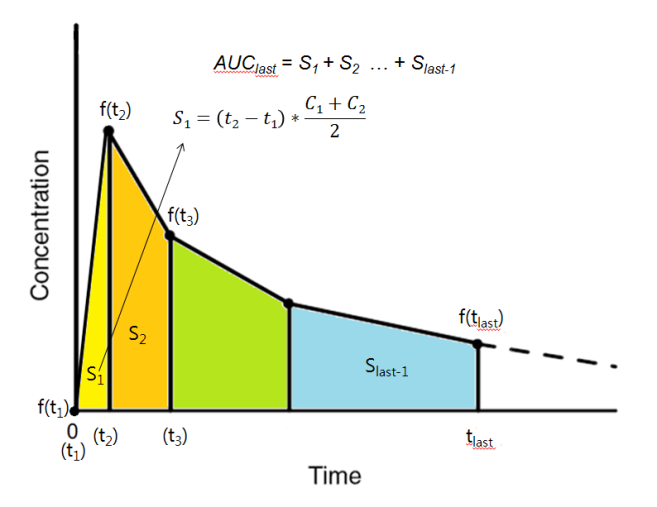
\includegraphics[width=9.12in]{assets/trapezoidal} \caption{Linear trapezoidal model}\label{fig:trapezoid}
\end{figure}

추가적으로 마지막으로 농도를 잰 시점에서 모든 약물이 우리 몸에서
빠져나가는 시점까지의 값을 구하기 위해서 마지막으로 측정한 점의 기울기가
그대로 약물이 모두 제거되는 시점까지 그대로 유지된다는 가정을 세우게
됩니다. 다음과 같이 C\textsubscript{last}(가장 마지막으로 농도를 측정한
시점)에서 λ (C\textsubscript{max} 이후에 선형성이 가장 높은 3점을
선택하여 구한 기울기)를 구한 후 다음과 같은 약동학 공식을 대입하여 값을
구해주게 됩니다.

\[
AUC_{t_{last}-\infty} = 
  \frac{C_{last}}{\lambda} \\
AUMC_{t_{last}-\infty} = 
  \frac{t_{last} \cdot C_{last}}{\lambda} + 
  \frac{C_{last}}{\lambda^2}
\]

약물이 우리 몸에 들어온 후 가장 높은 농도의 경우 실제 개개인에서 농도를
측정한 값들 중 가장 높은 농도를 실제 가장 높은 농도라 가정하여 사용하게
되고, 이 지표를 C\textsubscript{max}라 부릅니다. 또한 이때의 시점을
T\textsubscript{max}라 부르게 됩니다. 위에서 구한 AUC와
C\textsubscript{max}, λ 를 가지고 나머지 주요 값을 계산하게 됩니다. 이
중 청소율(제거되는 속도)에 해당하는 clearance(일반적으로 CL이라
지칭한다.) 의 경우 다음의 약동학 기본 공식을 활용하여 구해주게 됩니다.

\[
CL = \frac{D \cdot F}{AUC}
\]

수식에서 D는 dose로 투여량을, F는 생체이용률을 의미합니다.

우리 몸의 분포 (disposition)을 알기 위해 우리 몸의 volume을 나타내는
volume of distribution at steady state (Vdss)는 아래 식을 이용하여 값을
구하게 됩니다.

\[
Vd_{ss} = MRT \cdot CL = \frac{AUMC}{AUC} \cdot \frac{D}{AUC}
\]

우리 몸의 생체이용률을 나타내는 F의 경우 기본적으로 정맥주사시의
생체이용률을 1이라고 가정하고, 다음 식으로 구합니다.

\[
F = \frac{D_{iv}}{D_{oral}} \cdot \frac{AUC_{oral}}{AUC_{iv}}
\]

(이중 Div는 정맥주사 투여량, Doral은 경구 투여량, AUCoral은 경구
투여에서의 AUC, AUCiv는 정맥투여에서의 AUC를 의미한다.) 이처럼 AUC,
C\textsubscript{max}, AUMC, λ 를 구하는 부분에 있어서는
non-compartmental analysis의 기본 가정들을 활용하였고 그 밖의
부분들에서는 현재 정형화된 공식들을 활용하여 적용하였다. 위 내용을
바탕으로 R을 기반으로 한 script를 구성한 후 전세계적으로 널리 쓰이고
있는 CDISC terminology를 각각의 지표들에 적용하여 결과값을 도출하였다.

또한 투여되는 방식을 3가지 분류(Extravascular, IV infusion, IV bolus)로
구분하여, 그에 맞는 각각의 식을 적용하였다. 마지막으로 시간당 농도의
변화율이 농도 증가 곡선보다 감소 곡선에서 완만하다는 점을 고려하여
농도가 감소하는 구간에서는 log값을 선택적으로 줄 수 있도록 설정하였으며,
흡수 속도 상수의 경우 현 NCA method를 통해 구하기에는 한계가 있어 따로
값을 제시하지 않았습니다.

흡수속도 상수를 구하기 위해서는 구획분석방법(compartmental analysis)이나
비선형 혼합모형(non-linear mixed effect modeling)을 사용하는 것이
바람직합니다.

Figure 2. Linear trapezoidal method를 적용한 AUC의 계산 Script

Figure 3 약동학 지표들에 대해 각각의 공식을 적용한 Script의 예

\chapter{R과 그 패키지에 대하여}\label{R-and-packages}

\section{이 장에서는}\label{summary-r-packages}

R (R Core Team \protect\hyperlink{ref-R-base}{2017})은 통계 소프트웨어
입니다. 굉장히 유용한 소프트웨어이지만 이에 대해 여기서 자세히 설명하긴
힘듭니다. R에 대한 많은 책들을 bookdown.org\footnote{\url{https://bookdown.org}}에서
무료로 읽을 수 있습니다.

또한 이 책에서 주로 다루게 될 \texttt{NonCompart} (Bae
\protect\hyperlink{ref-R-NonCompart}{2017}\protect\hyperlink{ref-R-NonCompart}{b}),
\texttt{ncar} (Bae
\protect\hyperlink{ref-R-ncar}{2017}\protect\hyperlink{ref-R-ncar}{a}),
\texttt{pkr} (Bae and Lee \protect\hyperlink{ref-R-pkr}{2017}) 은 비구획
분석을 R을 통해 쉽고 빠르게 (매우 빠르게) 행할 수 있는 R 패키지입니다.

\texttt{NonCompart}의 패키지 제목은 Noncompartmental Analysis for
Pharmacokinetic Data, \texttt{ncar}의 패키지 제목은 Noncompartmental
Analysis for Pharmacokinetic Report, \texttt{pkr}의 패키지 제목은
Pharmacokinetics in R 입니다.

\section{설치}\label{install}

우선 R을 설치합니다. R은 아래 링크에서 다운로드 받을 수 있습니다.
\url{https://r-project.org/}

R을 실행한 후, 아래와 같이 패키지를 설치합니다.

\begin{Shaded}
\begin{Highlighting}[]
\KeywordTok{install.packages}\NormalTok{(}\StringTok{'NonCompart'}\NormalTok{)}
\KeywordTok{install.packages}\NormalTok{(}\StringTok{'ncar'}\NormalTok{)}
\KeywordTok{install.packages}\NormalTok{(}\StringTok{'pkr'}\NormalTok{)}
\end{Highlighting}
\end{Shaded}

이제 아래와 같이 입력하여 패키지를 불러올 수 있습니다.

\begin{Shaded}
\begin{Highlighting}[]
\KeywordTok{library}\NormalTok{(NonCompart)}
\KeywordTok{library}\NormalTok{(ncar)}
\KeywordTok{library}\NormalTok{(pkr)}
\end{Highlighting}
\end{Shaded}

\section{기타 설치}\label{-}

자료 분석을 위해 몇가지 도구가 필요한데 \texttt{tidyverse}(Wickham
\protect\hyperlink{ref-R-tidyverse}{2017})를 설치하면 다수의 편리한
패키지(Wickham and Henry \protect\hyperlink{ref-R-tidyr}{2017}; Wickham
et al. \protect\hyperlink{ref-R-dplyr}{2017}; Müller and Wickham
\protect\hyperlink{ref-R-tibble}{2017}; Wickham and Chang
\protect\hyperlink{ref-R-ggplot2}{2016}; Henry and Wickham
\protect\hyperlink{ref-R-purrr}{2017}; Wickham, Hester, and Francois
\protect\hyperlink{ref-R-readr}{2017})의 설치와 불러오기 과정을 쉽게
끝낼 수 있습니다. 이 책에서는 이를 주로 사용하겠습니다.\\
다음과 같이 설치하고 불러올 수 있습니다. 다만 비구획분석을 위한 함수의
입력을 위해 \texttt{tibble} 형식은 \texttt{as.data.frame()}을 통하여
데이타프레임으로 자료 형식을 변환하는 것이 좋습니다.

\begin{Shaded}
\begin{Highlighting}[]
\KeywordTok{install.packages}\NormalTok{(}\StringTok{'devtools'}\NormalTok{)}
\NormalTok{devtools}\OperatorTok{::}\KeywordTok{install_github}\NormalTok{(}\StringTok{'tidyverse/tidyverse'}\NormalTok{)}
\KeywordTok{library}\NormalTok{(tidyverse)}
\end{Highlighting}
\end{Shaded}

\section{기본적인 R 사용법}\label{basic}

R의 사용법을 익히는 것은 여러모로 유용합니다. 특히 자료의 재현가능한
편집이라는 측면이 가장 중요합니다. 오류를 줄일 수 있고, 한번 설정한 것을
반복해서 적용하는 것이 쉽기 때문입니다.

\chapter{R을 사용한 비구획분석}\label{noncompart}

\section{이 장에서는}\label{summary-noncompart}

\texttt{NonCompart} (Bae
\protect\hyperlink{ref-R-NonCompart}{2017}\protect\hyperlink{ref-R-NonCompart}{b})은
비구획 분석을 R을 통해 쉽고 빠르게 (매우 빠르게) 행할 수 있는
패키지입니다. 이에 대해 좀더 자세히 알아보겠습니다.

\texttt{NonCompart}의 \texttt{DESCRIPTION} 파일을 보면 다음과 같이
설명하고 있습니다.

\begin{quote}
Conduct a noncompartmental analysis as closely as possible to the most
widely used commercial software for pharmacokinetic analysis, i.e.
`Phoenix(R) WinNonlin(R)'
\url{https://www.certara.com/software/pkpd-modeling-and-simulation/phoenix-winnonlin/}.
Some features are 1) Use of CDISC SDTM terms 2) Automatic slope
selection with the same criterion of WinNonlin(R) 3) Supporting both
`linear-up linear-down' and `linear-up log-down' method 4)
Interval(partial) AUCs with `linear' or `log' interpolation method *
Reference: Gabrielsson J, Weiner D. Pharmacokinetic and Pharmacodynamic
Data Analysis - Concepts and Applications. 5th ed. 2016.
(\url{ISBN:9198299107}).
\end{quote}

\begin{Shaded}
\begin{Highlighting}[]
\KeywordTok{library}\NormalTok{(tidyverse)}
\KeywordTok{library}\NormalTok{(NonCompart)}
\KeywordTok{library}\NormalTok{(ncar)}
\end{Highlighting}
\end{Shaded}

\section{데이타에 대해}\label{TheophData}

R에는 theophylline과 Indomethacin의 약동학 데이터가 내장되어 있습니다.

\begin{itemize}
\tightlist
\item
  \texttt{Theoph}: theophylline의 약동학 데이터, 12명, 320mg PO
  단회투여, 0\textasciitilde{}24시간 채혈, NONMEM 의 run 폴더의 THEOPP
  데이터와 동일합니다.
\item
  \texttt{Indometh}: Indomethacin의 약동학 데이터, 6명, 25mg IV bolus
  단회투여, 0\textasciitilde{}8시간 채혈(0, 0.25, 0.5, 0.75, 1, 1.25, 2,
  3, 4, 5, 6, 8 h) (데이터명의 첫글짜가 대문자임에 주의하길)
\end{itemize}

먼저 데이터를 살펴보겠습니다.

\begin{Shaded}
\begin{Highlighting}[]
\KeywordTok{head}\NormalTok{(Theoph)}
\end{Highlighting}
\end{Shaded}

\begin{verbatim}
## Grouped Data: conc ~ Time | Subject
##   Subject   Wt Dose Time  conc
## 1       1 79.6 4.02 0.00  0.74
## 2       1 79.6 4.02 0.25  2.84
## 3       1 79.6 4.02 0.57  6.57
## 4       1 79.6 4.02 1.12 10.50
## 5       1 79.6 4.02 2.02  9.66
## 6       1 79.6 4.02 3.82  8.58
\end{verbatim}

\begin{Shaded}
\begin{Highlighting}[]
\KeywordTok{tail}\NormalTok{(Theoph)}
\end{Highlighting}
\end{Shaded}

\begin{verbatim}
## Grouped Data: conc ~ Time | Subject
##     Subject   Wt Dose  Time conc
## 127      12 60.5  5.3  3.52 9.75
## 128      12 60.5  5.3  5.07 8.57
## 129      12 60.5  5.3  7.07 6.59
## 130      12 60.5  5.3  9.03 6.11
## 131      12 60.5  5.3 12.05 4.57
## 132      12 60.5  5.3 24.15 1.17
\end{verbatim}

다음과 같이 테스트 할 수 있습니다.

\begin{Shaded}
\begin{Highlighting}[]
\NormalTok{TheophNca <-}\StringTok{ }\KeywordTok{tblNCA}\NormalTok{(Theoph, }\DataTypeTok{key=}\StringTok{"Subject"}\NormalTok{, }\DataTypeTok{dose=}\DecValTok{320}\NormalTok{, }\DataTypeTok{concUnit=}\StringTok{"mg/L"}\NormalTok{)}
\KeywordTok{head}\NormalTok{(TheophNca)}
\end{Highlighting}
\end{Shaded}

\begin{verbatim}
##      Subject b0                 CMAX   CMAXD        TMAX   TLAG CLST  
## [1,] "1"     "2.36878509420585" "10.5" "0.0328125"  "1.12" "0"  "3.28"
## [2,] "2"     "2.41123733696293" "8.33" "0.02603125" "1.92" "0"  "0.9" 
## [3,] "3"     "2.52971150145858" "8.2"  "0.025625"   "1.02" "0"  "1.05"
## [4,] "4"     "2.59275546723663" "8.6"  "0.026875"   "1.07" "0"  "1.15"
## [5,] "5"     "2.55109229061238" "11.4" "0.035625"   "1"    "0"  "1.57"
## [6,] "6"     "2.0334043955261"  "6.44" "0.020125"   "1.15" "0"  "0.92"
##      CLSTP               TLST    LAMZHL             LAMZ                
## [1,] "3.28014647414312"  "24.37" "14.304377571097"  "0.0484569969657749"
## [2,] "0.888639849106919" "24.3"  "6.65934156262252" "0.104086443688432" 
## [3,] "1.05509670837553"  "24.17" "6.76608737718236" "0.102444314109434" 
## [4,] "1.15642160174997"  "24.65" "6.98124666099893" "0.0992870205306231"
## [5,] "1.55569511595616"  "24.35" "8.0022640410078"  "0.0866188839818201"
## [6,] "0.941271173708175" "23.85" "7.89499786796582" "0.0877957400561702"
##      LAMZLL LAMZUL  LAMZNPT CORRXY               R2                 
## [1,] "9.05" "24.37" "3"     "-0.99999986483748"  "0.999999729674979"
## [2,] "7.03" "24.3"  "4"     "-0.998596709529913" "0.99719538828397" 
## [3,] "9"    "24.17" "3"     "-0.999662423945811" "0.999324961849213"
## [4,] "9.02" "24.65" "3"     "-0.999461923749821" "0.998924137025692"
## [5,] "7.02" "24.35" "4"     "-0.999323363372814" "0.998647184582752"
## [6,] "2.03" "23.85" "7"     "-0.999120281624298" "0.998241337153017"
##      R2ADJ               AUCLST      AUCALL      AUCIFO            
## [1,] "0.999999459349959" "148.92305" "148.92305" "216.611933038226"
## [2,] "0.995793082425955" "91.5268"   "91.5268"   "100.173459143183"
## [3,] "0.998649923698427" "99.2865"   "99.2865"   "109.535970740547"
## [4,] "0.997848274051385" "106.7963"  "106.7963"  "118.378881427603"
## [5,] "0.997970776874129" "121.2944"  "121.2944"  "139.419777837118"
## [6,] "0.99788960458362"  "73.77555"  "73.77555"  "84.2544183301878"
##      AUCIFOD             AUCIFP             AUCIFPD            
## [1,] "0.676912290744456" "216.614955803818" "0.67692173688693" 
## [2,] "0.313042059822447" "100.064317640308" "0.312700992625963"
## [3,] "0.342299908564208" "109.585721753278" "0.342455380478994"
## [4,] "0.369934004461258" "118.44355857992"  "0.370136120562249"
## [5,] "0.435686805740995" "139.254630430615" "0.435170720095671"
## [6,] "0.263295057281837" "84.4966985785753" "0.264052183058048"
##      AUCPEO             AUCPEP             AUMCLST       
## [1,] "31.2489169404534" "31.2498763313113" "1459.0711035"
## [2,] "8.63168669340252" "8.53203003991598" "706.586566"  
## [3,] "9.3571734209797"  "9.39832451573008" "803.18587"   
## [4,] "9.7843308603032"  "9.83359392402986" "901.0842105" 
## [5,] "13.0005786254328" "12.8974026752838" "1017.1143165"
## [6,] "12.4371736674055" "12.688245527848"  "609.1523875" 
##      AUMCIFO            AUMCIFP            AUMCPEO           
## [1,] "4505.53481941065" "4505.67086458209" "67.6160286851172"
## [2,] "999.772287999786" "996.071583509104" "29.3252499112927"
## [3,] "1150.96476871455" "1152.65289026304" "30.2162940315685"
## [4,] "1303.25240140958" "1305.4981091996"  "30.8588106551423"
## [5,] "1667.72161189007" "1661.79367436228" "39.011744571249" 
## [6,] "978.428485741731" "986.966459689532" "37.7417566662308"
##      AUMCPEP            VZFO               VZFP              
## [1,] "67.6170064935417" "30.4867482345887" "30.4863228055447"
## [2,] "29.0626720309864" "30.6904415765423" "30.7239160557228"
## [3,] "30.318495985664"  "28.5170999496524" "28.5041534217657"
## [4,] "30.9777467963968" "27.2259641330176" "27.2110971545992"
## [5,] "38.7941877387202" "26.4979946505636" "26.5294196385914"
## [6,] "38.280335514986"  "43.2597344953234" "43.135694392041" 
##      CLFO               CLFP               MRTEVLST          
## [1,] "1.47729626669981" "1.47727565168591" "9.79748335465867"
## [2,] "3.19445891892989" "3.19794315842211" "7.71999639449866"
## [3,] "2.92141474473231" "2.92008844656286" "8.08957783787323"
## [4,] "2.70318485984093" "2.70170876184947" "8.43741038313125"
## [5,] "2.29522672438806" "2.29794872178016" "8.38550103302378"
## [6,] "3.79802040465035" "3.78713021198604" "8.25683288704727"
##      MRTEVIFO           MRTEVIFP          
## [1,] "20.8000305256292" "20.8003683211179"
## [2,] "9.98041094468705" "9.95431345556755"
## [3,] "10.5076420187191" "10.5182762117325"
## [4,] "11.0091630001303" "11.0221115006327"
## [5,] "11.9618725389051" "11.9334895308224"
## [6,] "11.612785479182"  "11.6805328053348"
\end{verbatim}

이는 문자(character)로 구성된 matrix로 구성된 결과물과 단위 정보가 담긴
attribute를 포함하고 있습니다.

데이터가 Subject, weight, Dose, Time, Concentration 으로 구성되었음을 알
수 있습니다.

이 패키지로 NCA 비구획방법으로 약동학 파라미터를 산출하기 위해서는
아래와 같이 하면 됩니다. 우선 Theophilline 의 약동학 파라미터를
구해보겠습니다.

\begin{Shaded}
\begin{Highlighting}[]
\NormalTok{NonCompart}\OperatorTok{::}\KeywordTok{tblNCA}\NormalTok{(Theoph, }\StringTok{"Subject"}\NormalTok{, }\StringTok{"Time"}\NormalTok{, }\StringTok{"conc"}\NormalTok{, }\DataTypeTok{dose=}\DecValTok{320}\NormalTok{)}
\end{Highlighting}
\end{Shaded}

\begin{verbatim}
##       Subject b0                 CMAX    CMAXD        TMAX   TLAG CLST  
##  [1,] "1"     "2.36878509420585" "10.5"  "0.0328125"  "1.12" "0"  "3.28"
##  [2,] "2"     "2.41123733696293" "8.33"  "0.02603125" "1.92" "0"  "0.9" 
##  [3,] "3"     "2.52971150145858" "8.2"   "0.025625"   "1.02" "0"  "1.05"
##  [4,] "4"     "2.59275546723663" "8.6"   "0.026875"   "1.07" "0"  "1.15"
##  [5,] "5"     "2.55109229061238" "11.4"  "0.035625"   "1"    "0"  "1.57"
##  [6,] "6"     "2.0334043955261"  "6.44"  "0.020125"   "1.15" "0"  "0.92"
##  [7,] "7"     "2.28854976005424" "7.09"  "0.02215625" "3.48" "0"  "1.15"
##  [8,] "8"     "2.17040271754659" "7.56"  "0.023625"   "2.02" "0"  "1.25"
##  [9,] "9"     "2.12464810390587" "9.03"  "0.02821875" "0.63" "0"  "1.12"
## [10,] "10"    "2.65770546248091" "10.21" "0.03190625" "3.55" "0"  "2.42"
## [11,] "11"    "2.1475943307927"  "8"     "0.025"      "0.98" "0"  "0.86"
## [12,] "12"    "2.82449347826545" "9.75"  "0.03046875" "3.52" "0"  "1.17"
##       CLSTP               TLST    LAMZHL             LAMZ                
##  [1,] "3.28014647414312"  "24.37" "14.304377571097"  "0.0484569969657749"
##  [2,] "0.888639849106919" "24.3"  "6.65934156262252" "0.104086443688432" 
##  [3,] "1.05509670837553"  "24.17" "6.76608737718236" "0.102444314109434" 
##  [4,] "1.15642160174997"  "24.65" "6.98124666099893" "0.0992870205306231"
##  [5,] "1.55569511595616"  "24.35" "8.0022640410078"  "0.0866188839818201"
##  [6,] "0.941271173708175" "23.85" "7.89499786796582" "0.0877957400561702"
##  [7,] "1.16071921229933"  "24.22" "7.84666826130148" "0.0883364961379133"
##  [8,] "1.22852675835656"  "24.12" "8.51003788342506" "0.0814505399453019"
##  [9,] "1.11648311706515"  "24.43" "8.40599880716182" "0.0824586341803179"
## [10,] "2.41369227401111"  "23.7"  "9.24691582297898" "0.0749598237757766"
## [11,] "0.859806606884089" "24.08" "7.26123651504339" "0.0954585598642772"
## [12,] "1.17553904959565"  "24.15" "6.28650816367189" "0.110259489451627" 
##       LAMZLL LAMZUL  LAMZNPT CORRXY               R2                 
##  [1,] "9.05" "24.37" "3"     "-0.99999986483748"  "0.999999729674979"
##  [2,] "7.03" "24.3"  "4"     "-0.998596709529913" "0.99719538828397" 
##  [3,] "9"    "24.17" "3"     "-0.999662423945811" "0.999324961849213"
##  [4,] "9.02" "24.65" "3"     "-0.999461923749821" "0.998924137025692"
##  [5,] "7.02" "24.35" "4"     "-0.999323363372814" "0.998647184582752"
##  [6,] "2.03" "23.85" "7"     "-0.999120281624298" "0.998241337153017"
##  [7,] "6.98" "24.22" "4"     "-0.999334862622512" "0.998670167652754"
##  [8,] "3.53" "24.12" "6"     "-0.995496052943785" "0.991012391426654"
##  [9,] "8.8"  "24.43" "3"     "-0.99972179371205"  "0.999443664822839"
## [10,] "9.38" "23.7"  "3"     "-0.999754311749369" "0.999508683861454"
## [11,] "9.03" "24.08" "3"     "-0.999999127979356" "0.999998255959473"
## [12,] "9.03" "24.15" "3"     "-0.999698355328196" "0.9993968016459"  
##       R2ADJ               AUCLST      AUCALL      AUCIFO            
##  [1,] "0.999999459349959" "148.92305" "148.92305" "216.611933038226"
##  [2,] "0.995793082425955" "91.5268"   "91.5268"   "100.173459143183"
##  [3,] "0.998649923698427" "99.2865"   "99.2865"   "109.535970740547"
##  [4,] "0.997848274051385" "106.7963"  "106.7963"  "118.378881427603"
##  [5,] "0.997970776874129" "121.2944"  "121.2944"  "139.419777837118"
##  [6,] "0.99788960458362"  "73.77555"  "73.77555"  "84.2544183301878"
##  [7,] "0.998005251479131" "90.7534"   "90.7534"   "103.771801796293"
##  [8,] "0.988765489283318" "88.55995"  "88.55995"  "103.906686815243"
##  [9,] "0.998887329645677" "86.32615"  "86.32615"  "99.9087179279482"
## [10,] "0.999017367722909" "138.3681"  "138.3681"  "170.652060635217"
## [11,] "0.999996511918946" "80.0936"   "80.0936"   "89.1027449234385"
## [12,] "0.998793603291801" "119.9775"  "119.9775"  "130.588831558118"
##       AUCIFOD             AUCIFP             AUCIFPD            
##  [1,] "0.676912290744456" "216.614955803818" "0.67692173688693" 
##  [2,] "0.313042059822447" "100.064317640308" "0.312700992625963"
##  [3,] "0.342299908564208" "109.585721753278" "0.342455380478994"
##  [4,] "0.369934004461258" "118.44355857992"  "0.370136120562249"
##  [5,] "0.435686805740995" "139.254630430615" "0.435170720095671"
##  [6,] "0.263295057281837" "84.4966985785753" "0.264052183058048"
##  [7,] "0.324286880613414" "103.893147024686" "0.324666084452144"
##  [8,] "0.324708396297635" "103.643051464786" "0.323884535827455"
##  [9,] "0.312214743524838" "99.8660676588793" "0.312081461433998"
## [10,] "0.533287689485054" "170.567912545332" "0.533024726704162"
## [11,] "0.278446077885745" "89.1007189855217" "0.278439746829755"
## [12,] "0.408090098619118" "130.639068046815" "0.408247087646298"
##       AUCPEO             AUCPEP             AUMCLST       
##  [1,] "31.2489169404534" "31.2498763313113" "1459.0711035"
##  [2,] "8.63168669340252" "8.53203003991598" "706.586566"  
##  [3,] "9.3571734209797"  "9.39832451573008" "803.18587"   
##  [4,] "9.7843308603032"  "9.83359392402986" "901.0842105" 
##  [5,] "13.0005786254328" "12.8974026752838" "1017.1143165"
##  [6,] "12.4371736674055" "12.688245527848"  "609.1523875" 
##  [7,] "12.5452209279821" "12.6473664538854" "782.41986"   
##  [8,] "14.7697297311878" "14.5529307094073" "739.534598"  
##  [9,] "13.5949777052926" "13.5580763078894" "705.2296255" 
## [10,] "18.9180022292417" "18.8780011813617" "1278.180042" 
## [11,] "10.1109622730249" "10.1089184106194" "617.2422125" 
## [12,] "8.12575733430562" "8.16108703637935" "977.8807235" 
##       AUMCIFO            AUMCIFP            AUMCPEO           
##  [1,] "4505.53481941065" "4505.67086458209" "67.6160286851172"
##  [2,] "999.772287999786" "996.071583509104" "29.3252499112927"
##  [3,] "1150.96476871455" "1152.65289026304" "30.2162940315685"
##  [4,] "1303.25240140958" "1305.4981091996"  "30.8588106551423"
##  [5,] "1667.72161189007" "1661.79367436228" "39.011744571249" 
##  [6,] "978.428485741731" "986.966459689532" "37.7417566662308"
##  [7,] "1245.09840831465" "1249.41106012833" "37.1599983764277"
##  [8,] "1298.11575468474" "1288.52011616077" "43.0301500208197"
##  [9,] "1201.77153812025" "1200.2123597462"  "41.3174964516894"
## [10,] "2473.99342735889" "2470.87654175199" "48.3353501320931"
## [11,] "928.559971386069" "928.489963582081" "33.5269415524517"
## [12,] "1330.38400236898" "1332.05283411623" "26.4963558071417"
##       AUMCPEP            VZFO               VZFP              
##  [1,] "67.6170064935417" "30486.7482345887" "30486.3228055447"
##  [2,] "29.0626720309864" "30690.4415765423" "30723.9160557228"
##  [3,] "30.318495985664"  "28517.0999496524" "28504.1534217657"
##  [4,] "30.9777467963968" "27225.9641330176" "27211.0971545992"
##  [5,] "38.7941877387202" "26497.9946505636" "26529.4196385914"
##  [6,] "38.280335514986"  "43259.7344953234" "43135.694392041" 
##  [7,] "37.376906210544"  "34908.4408430805" "34867.6684452056"
##  [8,] "42.605894256157"  "37810.5081118408" "37906.6861615621"
##  [9,] "41.2412628670872" "38842.7934436931" "38859.3822173436"
## [10,] "48.2701777931124" "25015.5401378403" "25027.8813214113"
## [11,] "33.5219295081337" "37622.1852019531" "37623.0406407462"
## [12,] "26.5884431567018" "22224.2935639128" "22215.7473419508"
##       CLFO               CLFP               MRTEVLST          
##  [1,] "1477.29626669981" "1477.27565168591" "9.79748335465867"
##  [2,] "3194.45891892989" "3197.94315842211" "7.71999639449866"
##  [3,] "2921.41474473231" "2920.08844656286" "8.08957783787323"
##  [4,] "2703.18485984093" "2701.70876184947" "8.43741038313125"
##  [5,] "2295.22672438806" "2297.94872178016" "8.38550103302378"
##  [6,] "3798.02040465035" "3787.13021198604" "8.25683288704727"
##  [7,] "3083.68934971535" "3080.08765894795" "8.62138344128154"
##  [8,] "3079.68630131565" "3087.52005539633" "8.3506663903943" 
##  [9,] "3202.92369511514" "3204.29158273309" "8.1693626496722" 
## [10,] "1875.16048038837" "1876.08557333405" "9.23753409926132"
## [11,] "3591.35961832556" "3591.44127728081" "7.70651103833515"
## [12,] "2450.4392617801"  "2449.49695970983" "8.15053425433936"
##       MRTEVIFO           MRTEVIFP          
##  [1,] "20.8000305256292" "20.8003683211179"
##  [2,] "9.98041094468705" "9.95431345556755"
##  [3,] "10.5076420187191" "10.5182762117325"
##  [4,] "11.0091630001303" "11.0221115006327"
##  [5,] "11.9618725389051" "11.9334895308224"
##  [6,] "11.612785479182"  "11.6805328053348"
##  [7,] "11.9984271908357" "12.0259237101698"
##  [8,] "12.4930915850769" "12.4322865638375"
##  [9,] "12.0286954236259" "12.0182198807093"
## [10,] "14.4972959491374" "14.4861744795951"
## [11,] "10.4212274513421" "10.4206786898426"
## [12,] "10.1875787270284" "10.1964355229393"
## attr(,"units")
##  [1] ""          ""          "ug/L"      "ug/L/mg"   "h"        
##  [6] "h"         "ug/L"      "ug/L"      "h"         "h"        
## [11] "/h"        "h"         "h"         ""          ""         
## [16] ""          ""          "h*ug/L"    "h*ug/L"    "h*ug/L"   
## [21] "h*ug/L/mg" "h*ug/L"    "h*ug/L/mg" "%"         "%"        
## [26] "h2*ug/L"   "h2*ug/L"   "h2*ug/L"   "%"         "%"        
## [31] "L"         "L"         "L/h"       "L/h"       "h"        
## [36] "h"         "h"
\end{verbatim}

다음으로 Indomethacin 의 약동학 파라미터를 구해보자. 이는 IV bolus
이므로 AdmMode 옵션이 추가된다.

\begin{Shaded}
\begin{Highlighting}[]
\NormalTok{NonCompart}\OperatorTok{::}\KeywordTok{tblNCA}\NormalTok{(Indometh, }\StringTok{"Subject"}\NormalTok{, }\StringTok{"time"}\NormalTok{, }\StringTok{"conc"}\NormalTok{, }\DataTypeTok{dose=}\DecValTok{25}\NormalTok{, }\DataTypeTok{adm=}\StringTok{"Bolus"}\NormalTok{, }\DataTypeTok{dur=}\FloatTok{0.5}\NormalTok{, }\DataTypeTok{concUnit=}\StringTok{"mg/L"}\NormalTok{)}
\end{Highlighting}
\end{Shaded}

\begin{verbatim}
##      Subject b0                    CMAX   CMAXD    TMAX   TLAG CLST  
## [1,] "1"     "-1.72421059639646"   "1.5"  "0.06"   "0.25" NA   "0.05"
## [2,] "2"     "-0.175286858431038"  "2.03" "0.0812" "0.25" NA   "0.08"
## [3,] "3"     "0.155579544657487"   "2.72" "0.1088" "0.25" NA   "0.08"
## [4,] "4"     "0.200296947923903"   "1.85" "0.074"  "0.25" NA   "0.07"
## [5,] "5"     "-0.982357129866236"  "2.05" "0.082"  "0.25" NA   "0.06"
## [6,] "6"     "-0.0499189799474626" "2.31" "0.0924" "0.25" NA   "0.09"
##      CLSTP                TLST LAMZHL             LAMZ               
## [1,] "0.0502485064135143" "8"  "4.37812701206528" "0.158320482400297"
## [2,] "0.0747559092002026" "8"  "2.293063170278"   "0.302280019819912"
## [3,] "0.0399725765960521" "8"  "1.64294680807057" "0.421892648718165"
## [4,] "0.0319601103599335" "8"  "1.52191040768299" "0.455445456618709"
## [5,] "0.0495714902818329" "8"  "2.74244612209262" "0.252747784168332"
## [6,] "0.0562424678832525" "8"  "1.9606985693831"  "0.353520521401732"
##      LAMZLL LAMZUL LAMZNPT CORRXY               R2                 
## [1,] "5"    "8"    "3"     "-0.998532286621828" "0.997066727426216"
## [2,] "0.75" "8"    "9"     "-0.973482979595454" "0.947669111562043"
## [3,] "0.5"  "8"    "10"    "-0.935855785859431" "0.875826051926574"
## [4,] "0.25" "8"    "11"    "-0.93425095790181"  "0.872824852340449"
## [5,] "1"    "8"    "8"     "-0.935544879811905" "0.875244222142273"
## [6,] "0.75" "8"    "9"     "-0.950764854539454" "0.903953808627429"
##      R2ADJ               AUCLST             AUCALL            
## [1,] "0.994133454852432" "2.04045212765957" "2.04045212765957"
## [2,] "0.94019327035662"  "3.24851993865031" "3.24851993865031"
## [3,] "0.860304308417395" "3.5544211409396"  "3.5544211409396" 
## [4,] "0.858694280378276" "2.78527877697842" "2.78527877697842"
## [5,] "0.854451592499318" "2.45885817307692" "2.45885817307692"
## [6,] "0.890232924145633" "3.335703125"      "3.335703125"     
##      AUCIFO             AUCIFOD              AUCIFP            
## [1,] "2.356267234094"   "0.0942506893637602" "2.35783687568268"
## [2,] "3.51317520778672" "0.140527008311469"  "3.49582675451177"
## [3,] "3.74404283793542" "0.149761713517417"  "3.64916698853258"
## [4,] "2.93897445882733" "0.117558978353093"  "2.85545207631751"
## [5,] "2.69624897829181" "0.107849959131673"  "2.6549884396387" 
## [6,] "3.59028523424544" "0.143611409369818"  "3.4947956372543" 
##      AUCIFPD              AUCPEO             AUCPEP             AUMCLST   
## [1,] "0.0943134750273071" "13.4031956080679" "13.4608441871624" "3.27125" 
## [2,] "0.139833070180471"  "7.53322147298048" "7.07434416028442" "6.39875" 
## [3,] "0.145966679541303"  "5.064624129685"   "2.59636919578418" "5.00625" 
## [4,] "0.1142180830527"    "5.22956847710184" "2.45751977142578" "4.381875"
## [5,] "0.106199537585548"  "8.80448382646355" "7.3872361790195"  "3.7075"  
## [6,] "0.139791825490172"  "7.09086026973962" "4.55226939619547" "5.5325"  
##      AUMCIFO            AUMCIFP            AUMCPEO           
## [1,] "7.79255448051925" "7.81502594373644" "58.0208260567461"
## [2,] "9.39152229661219" "9.19534267578028" "31.8667432402495"
## [3,] "6.97267842561125" "5.9887901357925"  "28.2019090166038"
## [4,] "5.94890277791985" "5.09733758170571" "26.3414588608858"
## [5,] "6.54586634839538" "6.05253416426272" "43.3612022813628"
## [6,] "8.28929076671746" "7.25526351286615" "33.2572573975366"
##      AUMCPEP            C0                 AUCPBEO           
## [1,] "58.1415337127341" "2.3936170212766"  "20.6556421367339"
## [2,] "30.4131425481974" "2.52815950920245" "16.2180906146511"
## [3,] "16.4063210350329" "4.96536912751678" "25.6586578338762"
## [4,] "14.0360054682958" "2.46223021582734" "18.3407098132283"
## [5,] "38.7446662938147" "4.04086538461538" "28.2376805408852"
## [6,] "23.7450164258139" "3.705625"         "20.9441054384092"
##      AUCPBEP            VZO                VZP               
## [1,] "20.6418914166255" "67.0159780403394" "66.9713646630007"
## [2,] "16.2985748053719" "23.541317103064"  "23.6581436704179"
## [3,] "26.3257654132706" "15.8269504052657" "16.2384403063513"
## [4,] "18.8771782040751" "18.6770302753637" "19.2233360879334"
## [5,] "28.6765155625511" "36.6853492769315" "37.2554674926062"
## [6,] "21.5163689969229" "19.6968340826101" "20.2350179834082"
##      CLO                CLP                MRTIVLST          
## [1,] "10.6100019718742" "10.6029387604525" "1.35319860272937"
## [2,] "7.11606980050102" "7.15138413759623" "1.7197431817699" 
## [3,] "6.67727402760856" "6.85087859189834" "1.15845718655517"
## [4,] "8.5063685820445"  "8.75518108230375" "1.32322672194186"
## [5,] "9.27214074118575" "9.41623685691155" "1.2578136838452" 
## [6,] "6.96323505484772" "7.15349410806788" "1.40857085977938"
##      MRTIVIFO           MRTIVIFP           VSSO              
## [1,] "3.05716073616986" "3.06448965971139" "32.4364814390986"
## [2,] "2.42322912782616" "2.38037711005347" "17.2438676162182"
## [3,] "1.61233938216802" "1.39113896530691" "10.766031880241" 
## [4,] "1.77414238750939" "1.53512454261863" "15.0915090651833"
## [5,] "2.17776776221254" "2.02968381100988" "20.1925691928519"
## [6,] "2.0588112018653"  "1.82601939167072" "14.3359863321416"
##      VSSP              
## [1,] "32.4925961939597"
## [2,] "17.0229911063336"
## [3,] "9.53052415577672"
## [4,] "13.4402933545148"
## [5,] "19.1119835091079"
## [6,] "13.0624189595342"
## attr(,"units")
##  [1] ""          ""          "mg/L"      "mg/L/mg"   "h"        
##  [6] "h"         "mg/L"      "mg/L"      "h"         "h"        
## [11] "/h"        "h"         "h"         ""          ""         
## [16] ""          ""          "h*mg/L"    "h*mg/L"    "h*mg/L"   
## [21] "h*mg/L/mg" "h*mg/L"    "h*mg/L/mg" "%"         "%"        
## [26] "h2*mg/L"   "h2*mg/L"   "h2*mg/L"   "%"         "%"        
## [31] "mg/L"      "%"         "%"         "L"         "L"        
## [36] "L/h"       "L/h"       "h"         "h"         "h"        
## [41] "L"         "L"
\end{verbatim}

\section{NonCompart 사용법}\label{how-to-use}

NCA의 사용법은 다음과 같습니다.

\texttt{NCA(Data,\ colSubj,\ colTime,\ colConc,\ colTrt,\ Method\ =\ "Linear",\ Dose\ =\ 0,\ AdmMode\ =\ "Extravascular",\ TimeInfusion\ =\ 0,\ Report\ =\ "Table",\ iAUC)}

Data는 데이터셋을 설정하며, colSubj는 subject ID의 컬럼명, colTime은
time의 컬럼명, colConc는 concentration의 컬럼명, colTrT는 treatment
code의 컬럼명(교차시험에서 사용)이다.

\begin{Shaded}
\begin{Highlighting}[]
\KeywordTok{tblNCA}\NormalTok{(concData, }\DataTypeTok{key =} \StringTok{"Subject"}\NormalTok{, }\DataTypeTok{colTime =} \StringTok{"Time"}\NormalTok{, }\DataTypeTok{colConc =} \StringTok{"conc"}\NormalTok{, }
       \DataTypeTok{dose =} \DecValTok{0}\NormalTok{, }\DataTypeTok{adm =} \StringTok{"Extravascular"}\NormalTok{, }\DataTypeTok{dur =} \DecValTok{0}\NormalTok{, }\DataTypeTok{doseUnit =} \StringTok{"mg"}\NormalTok{, }
       \DataTypeTok{timeUnit =} \StringTok{"h"}\NormalTok{, }\DataTypeTok{concUnit =} \StringTok{"ug/L"}\NormalTok{, }\DataTypeTok{down =} \StringTok{"Linear"}\NormalTok{, }\DataTypeTok{MW =} \DecValTok{0}\NormalTok{)}
\CommentTok{# args(NonCompart::tblNCA)}
\end{Highlighting}
\end{Shaded}

NCA의 옵션들에 대해서 간단히 살펴보자면 다음과 같습니다.

\begin{enumerate}
\def\labelenumi{\arabic{enumi}.}
\tightlist
\item
  \texttt{down}

  \begin{itemize}
  \tightlist
  \item
    AUC와 AUMC를 구하는 trapezoidal method 설정, 기본값은
    Method=``Linear''
  \item
    Linear와 Log 중 선택 가능하다.
  \item
    Linear는 Linear trapezoidal method이며, Log는 Linear-up and log-down
    method 입니다.
  \end{itemize}
\item
  \texttt{dose}

  \begin{itemize}
  \tightlist
  \item
    투여량에 대한 설정이다. 단위에 주의해야 한다. 벡터값을 줌으로서 각
    대상자별 용량을 다르게 할 수 있습니다.
  \end{itemize}
\item
  \texttt{adm}

  \begin{itemize}
  \tightlist
  \item
    투여경로에 대한 설정, 기본값은 ``Extravascular''으로 경구 투여 등을
    의미합니다.
  \item
    Bolus, Infusion, Extravascular 중에서 선택 가능하다.
  \end{itemize}
\item
  \texttt{dur}

  \begin{itemize}
  \tightlist
  \item
    주입하는 기간(infusion duration)을 설정한다. 기본값은 0이다.
  \end{itemize}
\end{enumerate}

\section{구간 NCA}\label{interval-NCA}

\begin{enumerate}
\def\labelenumi{\arabic{enumi}.}
\tightlist
\item
  iAUC

  \begin{itemize}
  \tightlist
  \item
    일부구간에 대한 AUC를 구하기 위한 구간설정 옵션입니다.
  \item
    ``Name'', ``Start'', ``End'' 3개의 컬럼으로 구성된 데이터 프레임으로
    설정해야 합니다.
  \end{itemize}
\end{enumerate}

일부 구간의 AUC를 구하는 방법은 조금 더 복잡하므로 자세히 알아봅시다.
예를 들어 0\textasciitilde{}12시간까지의 AUC,
0\textasciitilde{}24시간까지의 AUC를 구하고자 한다면 다음과 같이 하면
됩니다. 먼저 구하고자 하는 구간에 대한 정보를 갖는 변수를 아래와같이
생성합니다.

\begin{Shaded}
\begin{Highlighting}[]
\NormalTok{iAUC <-}\StringTok{ }\KeywordTok{data.frame}\NormalTok{(}\DataTypeTok{Name=}\KeywordTok{c}\NormalTok{(}\StringTok{"AUC[0-12h]"}\NormalTok{,}\StringTok{"AUC[0-24h]"}\NormalTok{), }\DataTypeTok{Start=}\KeywordTok{c}\NormalTok{(}\DecValTok{0}\NormalTok{,}\DecValTok{0}\NormalTok{), }\DataTypeTok{End=}\KeywordTok{c}\NormalTok{(}\DecValTok{12}\NormalTok{,}\DecValTok{24}\NormalTok{)) ; iAUC}
\end{Highlighting}
\end{Shaded}

\begin{verbatim}
##         Name Start End
## 1 AUC[0-12h]     0  12
## 2 AUC[0-24h]     0  24
\end{verbatim}

\begin{verbatim}
    Name Start End
\end{verbatim}

1 AUC{[}0-12h{]} 0 12 2 AUC{[}0-24h{]} 0 24

이제 iAUC 옵션을 이용해서 이를 구합니다.

\begin{Shaded}
\begin{Highlighting}[]
\CommentTok{# tblNCA(Theoph, "Subject", "Time", "conc", dose=320, iAUC=iAUC)}
\end{Highlighting}
\end{Shaded}

맨 마지막 파라미터로 AUC{[}0-12h{]}, AUC{[}0-24h{]}가 추가되었음을 알 수
있습니다.

\section{함수 살펴보기}\label{functions}

NonCompart 패키지 내의 여러가지 함수를 살펴보겠습니다. AUC(),
BestSlope(), IntAUC(), Interpol(), LinAUC(), LogAUC(), Slope(), sNCA(),
tblNCA(), Unit(), UnitUrine(), UT()라는 함수가 있습니다.

\subsection{AUC}\label{auc}

AUC와 AUMC를 `Linear trapezoidal method' 혹은 'linear-up and log-down
method'의 두가지 방식으로 계산하게 됩니다.

\begin{Shaded}
\begin{Highlighting}[]
\KeywordTok{AUC}\NormalTok{(Theoph[Theoph}\OperatorTok{$}\NormalTok{Subject}\OperatorTok{==}\DecValTok{1}\NormalTok{, }\StringTok{"Time"}\NormalTok{], Theoph[Theoph}\OperatorTok{$}\NormalTok{Subject}\OperatorTok{==}\DecValTok{1}\NormalTok{, }\StringTok{"conc"}\NormalTok{])}
\end{Highlighting}
\end{Shaded}

\begin{verbatim}
##             AUC        AUMC
##  [1,]   0.00000    0.000000
##  [2,]   0.44750    0.088750
##  [3,]   1.95310    0.801534
##  [4,]   6.64735    5.065382
##  [5,]  15.71935   19.138321
##  [6,]  32.13535   66.198241
##  [7,]  42.97695  114.461665
##  [8,]  58.25290  206.281512
##  [9,]  72.75650  322.298798
## [10,]  92.45055  528.521903
## [11,] 148.92305 1459.071104
\end{verbatim}

\begin{Shaded}
\begin{Highlighting}[]
\KeywordTok{AUC}\NormalTok{(Theoph[Theoph}\OperatorTok{$}\NormalTok{Subject}\OperatorTok{==}\DecValTok{1}\NormalTok{, }\StringTok{"Time"}\NormalTok{], Theoph[Theoph}\OperatorTok{$}\NormalTok{Subject}\OperatorTok{==}\DecValTok{1}\NormalTok{, }\StringTok{"conc"}\NormalTok{], }\DataTypeTok{down=}\StringTok{"Log"}\NormalTok{)}
\end{Highlighting}
\end{Shaded}

\begin{verbatim}
## Error in AUC(Theoph[Theoph$Subject == 1, "Time"], Theoph[Theoph$Subject == : 사용되지 않은 인자 (down = "Log")
\end{verbatim}

\section{긴 형식으로 변환하면서 단위 추가하기}\label{long-format}

NonCompart 패키지의 tblNCA()함수를 사용해서 비구획분석 결과를 내면
문자형식의 행렬이 생성되고 그 attr로 dimnames와 units를 갖는데 이를 long
format의 tidy data로 변환하는 방법은 다음과 같습니다.

\begin{Shaded}
\begin{Highlighting}[]
\NormalTok{ncares <-}\StringTok{ }\NormalTok{NonCompart}\OperatorTok{::}\KeywordTok{tblNCA}\NormalTok{(Theoph, }\DataTypeTok{key=}\StringTok{"Subject"}\NormalTok{, }\DataTypeTok{dose=}\DecValTok{320}\NormalTok{, }\DataTypeTok{concUnit=}\StringTok{"mg/L"}\NormalTok{)}
\KeywordTok{str}\NormalTok{(ncares)}
\end{Highlighting}
\end{Shaded}

\begin{verbatim}
##  chr [1:12, 1:37] "1" "2" "3" "4" "5" "6" "7" "8" "9" "10" "11" "12" ...
##  - attr(*, "dimnames")=List of 2
##   ..$ : NULL
##   ..$ : chr [1:37] "Subject" "b0" "CMAX" "CMAXD" ...
##  - attr(*, "units")= chr [1:37] "" "" "mg/L" "mg/L/mg" ...
\end{verbatim}

\begin{Shaded}
\begin{Highlighting}[]
\KeywordTok{left_join}\NormalTok{(}\KeywordTok{as_tibble}\NormalTok{(ncares) }\OperatorTok\StringTok{ }\NormalTok{tidyr}\OperatorTok{::}\KeywordTok{gather}\NormalTok{(PPTESTCD, PPORRES, }\OperatorTok{-}\NormalTok{Subject),}
          \KeywordTok{tibble}\NormalTok{(}\DataTypeTok{PPTESTCD =} \KeywordTok{attr}\NormalTok{(ncares, }\StringTok{'dimnames'}\NormalTok{)[[}\DecValTok{2}\NormalTok{]], }\DataTypeTok{UNIT =} \KeywordTok{attr}\NormalTok{(ncares, }\StringTok{'units'}\NormalTok{)),}
          \DataTypeTok{by =} \StringTok{'PPTESTCD'}\NormalTok{) }\OperatorTok\StringTok{ }
\StringTok{  }\KeywordTok{arrange}\NormalTok{(Subject, PPTESTCD) }\OperatorTok\StringTok{ }
\StringTok{  }\KeywordTok{head}\NormalTok{(}\DecValTok{20}\NormalTok{)}
\end{Highlighting}
\end{Shaded}

\begin{verbatim}
## # A tibble: 20 x 4
##    Subject PPTESTCD           PPORRES      UNIT
##      <chr>    <chr>             <chr>     <chr>
##  1       1   AUCALL         148.92305    h*mg/L
##  2       1   AUCIFO  216.611933038226    h*mg/L
##  3       1  AUCIFOD 0.676912290744456 h*mg/L/mg
##  4       1   AUCIFP  216.614955803818    h*mg/L
##  5       1  AUCIFPD  0.67692173688693 h*mg/L/mg
##  6       1   AUCLST         148.92305    h*mg/L
##  7       1   AUCPEO  31.2489169404534         %
##  8       1   AUCPEP  31.2498763313113         %
##  9       1  AUMCIFO  4505.53481941065   h2*mg/L
## 10       1  AUMCIFP  4505.67086458209   h2*mg/L
## 11       1  AUMCLST      1459.0711035   h2*mg/L
## 12       1  AUMCPEO  67.6160286851172         %
## 13       1  AUMCPEP  67.6170064935417         %
## 14       1       b0  2.36878509420585          
## 15       1     CLFO  1.47729626669981       L/h
## 16       1     CLFP  1.47727565168591       L/h
## 17       1     CLST              3.28      mg/L
## 18       1    CLSTP  3.28014647414312      mg/L
## 19       1     CMAX              10.5      mg/L
## 20       1    CMAXD         0.0328125   mg/L/mg
\end{verbatim}

\chapter{R을 사용한 비구획분석 보고서}\label{ncar}

\section{이 장에서는}\label{summary-ncar}

보고서를 일정한 형식으로 작성하여 다른 사람/기관과 공유하는 것은
중요합니다. 이를 \texttt{ncar} 패키지를 사용하여 좀더 쉽게 할 수
있습니다.

이에 대해 좀더 자세히 알아보겠습니다.

\texttt{ncar}의 \texttt{DESCRIPTION} 파일을 보면 다음과 같이 설명하고
있습니다.

\begin{quote}
Conduct a noncompartmental analysis as closely as possible to the most
widely used commercial software for pharmacokinetic analysis, i.e.
`Phoenix(R) WinNonlin(R)'
\url{https://www.certara.com/software/pkpd-modeling-and-simulation/phoenix-winnonlin/}.
Some features are 1) CDISC SDTM terms 2) Automatic slope selection with
the same criterion of WinNonlin(R) 3) Supporting both `linear-up
linear-down' and `linear-up log-down' method 4) Interval(partial) AUCs
with `linear' or `log' interpolation method 5) Produce pdf, rtf, text
report files. * Reference: Gabrielsson J, Weiner D. Pharmacokinetic and
Pharmacodynamic Data Analysis - Concepts and Applications. 5th ed. 2016.
(\url{ISBN:9198299107}).
\end{quote}

\begin{Shaded}
\begin{Highlighting}[]
\KeywordTok{library}\NormalTok{(tidyverse)}
\KeywordTok{library}\NormalTok{(ncar)}
\end{Highlighting}
\end{Shaded}

\section{txtNCA}\label{txtnca}

\begin{Shaded}
\begin{Highlighting}[]
\NormalTok{txtNCA_Theoph <-}\StringTok{ }\NormalTok{Theoph }\OperatorTok\StringTok{ }
\StringTok{  }\KeywordTok{as_tibble}\NormalTok{() }\OperatorTok\StringTok{ }
\StringTok{  }\KeywordTok{group_by}\NormalTok{(Subject) }\OperatorTok\StringTok{ }
\StringTok{  }\KeywordTok{summarise}\NormalTok{(}\DataTypeTok{res =} \KeywordTok{c}\NormalTok{(}\DataTypeTok{ID =}\NormalTok{ glue}\OperatorTok{::}\KeywordTok{glue}\NormalTok{(}\StringTok{'ID=\{unique(Subject)\}}\CharTok{\textbackslash{}n\textbackslash{}n}\StringTok{'}\NormalTok{),}
                   \KeywordTok{txtNCA}\NormalTok{(Time, }
\NormalTok{                         conc, }
                         \DataTypeTok{dose=}\DecValTok{320}\NormalTok{, }
                         \DataTypeTok{doseUnit=}\StringTok{"mg"}\NormalTok{, }
                         \DataTypeTok{concUnit=}\StringTok{"mg/L"}\NormalTok{, }
                         \DataTypeTok{timeUnit=}\StringTok{"h"}\NormalTok{)) }\OperatorTok\StringTok{ }\KeywordTok{paste}\NormalTok{(}\DataTypeTok{collapse =} \StringTok{'}\CharTok{\textbackslash{}n}\StringTok{'}\NormalTok{)) }\OperatorTok
\StringTok{  }\NormalTok{.}\OperatorTok{$}\NormalTok{res }\OperatorTok
\StringTok{  }\KeywordTok{paste}\NormalTok{(}\DataTypeTok{collapse =} \StringTok{'}\CharTok{\textbackslash{}n\textbackslash{}n\textbackslash{}n\textbackslash{}n\textbackslash{}n\textbackslash{}n}\StringTok{'}\NormalTok{)}
\NormalTok{txtNCA_Theoph}
\end{Highlighting}
\end{Shaded}

\begin{verbatim}
## [1] "ID=6\n\n                        NONCOMPARTMENTAL ANALYSIS REPORT\n                       Package version 0.3.7 (2017-08-16 KST)\n                          R version 3.4.2 (2017-09-28)\n\nDate and Time: 2017-11-07 02:13:26 NA\n\nCalculation Setting\n-------------------\nDrug Administration: Extravascular\nObservation count excluding trailing zero: 11\nDose at time 0: 320 mg\nAUC Calculation Method: Linear-up Linear-down\nWeighting for lambda z: Uniform (Ordinary Least Square, OLS)\nLambda z selection criterion: Heighest adjusted R-squared value with precision=1e-4\n\n\nFitting, AUC, AUMC Result\n-------------------------\n      Time         Conc.      Pred.   Residual       AUC       AUMC\n---------------------------------------------------------------------\n     0.0000       0.0000                           0.0000     0.0000\n     0.2700       1.2900                           0.1742     0.0470\n     0.5800       3.0800                           0.8515     0.3779\n     1.1500       6.4400                           3.5647     2.9977\n     2.0300 *     6.3200     6.3928 -7.284e-02     9.1791    11.9014\n     3.5700 *     5.5300     5.5844 -5.438e-02    18.3036    36.9816\n     5.0000 *     4.9400     4.9255 +1.450e-02    25.7897    68.7577\n     7.0000 *     4.0200     4.1323 -1.123e-01    34.7497   121.5977\n     9.2200 *     3.4600     3.4005 +5.948e-02    43.0525   188.2434\n    12.1000 *     2.7800     2.6408 +1.392e-01    52.0381   282.6199\n    23.8500 *     0.9200     0.9413 -2.127e-02    73.7756   609.1524\n\n*: Used for the calculation of Lambda z.\n\n\nCalculated Values\n-----------------\nCMAX       Max Conc                                        6.4400 mg/L\nCMAXD      Max Conc Norm by Dose                           0.0201 mg/L/mg\nTMAX       Time of CMAX                                    1.1500 h\nTLAG       Time Until First Nonzero Conc                   0.0000 h\nCLST       Last Nonzero Conc                               0.9200 mg/L\nCLSTP      Last Nonzero Conc Pred                          0.9413 mg/L\nTLST       Time of Last Nonzero Conc                      23.8500 h\nLAMZHL     Half-Life Lambda z                              7.8950 h\nLAMZ       Lambda z                                        0.0878 /h\nLAMZLL     Lambda z Lower Limit                            2.0300 h\nLAMZUL     Lambda z Upper Limit                           23.8500 h\nLAMZNPT    Number of Points for Lambda z                   7\nCORRXY     Correlation Between TimeX and Log ConcY        -0.9991 \nR2         R Squared                                       0.9982 \nR2ADJ      R Squared Adjusted                              0.9979 \nAUCLST     AUC to Last Nonzero Conc                       73.7756 h*mg/L\nAUCALL     AUC All                                        73.7756 h*mg/L\nAUCIFO     AUC Infinity Obs                               84.2544 h*mg/L\nAUCIFOD    AUC Infinity Obs Norm by Dose                   0.2633 h*mg/L/mg\nAUCIFP     AUC Infinity Pred                              84.4967 h*mg/L\nAUCIFPD    AUC Infinity Pred Norm by Dose                  0.2641 h*mg/L/mg\nAUCPEO     AUC %Extrapolation Obs                         12.4372 %\nAUCPEP     AUC %Extrapolation Pred                        12.6882 %\nAUMCLST    AUMC to Last Nonzero Conc                     609.1524 h2*mg/L\nAUMCIFO    AUMC Infinity Obs                             978.4285 h2*mg/L\nAUMCIFP    AUMC Infinity Pred                            986.9665 h2*mg/L\nAUMCPEO    AUMC %Extrapolation Obs                        37.7418 %\nAUMCPEP    AUMC % Extrapolation Pred                      38.2803 %\nVZFO       Vz Obs by F                                    43.2597 L\nVZFP       Vz Pred by F                                   43.1357 L\nCLFO       Total CL Obs by F                               3.7980 L/h\nCLFP       Total CL Pred by F                              3.7871 L/h\nMRTEVLST   MRT Extravasc to Last Nonzero Conc              8.2568 h\nMRTEVIFO   MRT Extravasc Infinity Obs                     11.6128 h\nMRTEVIFP   MRT Extravasc Infinity Pred                    11.6805 h\n\n\n\n\n\nID=7\n\n                        NONCOMPARTMENTAL ANALYSIS REPORT\n                       Package version 0.3.7 (2017-08-16 KST)\n                          R version 3.4.2 (2017-09-28)\n\nDate and Time: 2017-11-07 02:13:26 NA\n\nCalculation Setting\n-------------------\nDrug Administration: Extravascular\nObservation count excluding trailing zero: 11\nDose at time 0: 320 mg\nAUC Calculation Method: Linear-up Linear-down\nWeighting for lambda z: Uniform (Ordinary Least Square, OLS)\nLambda z selection criterion: Heighest adjusted R-squared value with precision=1e-4\n\n\nFitting, AUC, AUMC Result\n-------------------------\n      Time         Conc.      Pred.   Residual       AUC       AUMC\n---------------------------------------------------------------------\n     0.0000       0.1500                           0.0000     0.0000\n     0.2500       0.8500                           0.1250     0.0266\n     0.5000       2.3500                           0.5250     0.2000\n     1.0200       5.0200                           2.4412     1.8368\n     2.0200       6.5800                           8.2412    11.0428\n     3.4800       7.0900                          18.2203    38.7571\n     5.0000       6.6600                          28.6703    82.8167\n     6.9800 *     5.2500     5.3226 -7.260e-02    40.4612   152.0623\n     9.0000 *     4.3900     4.4527 -6.275e-02    50.1976   228.9788\n    12.0500 *     3.5300     3.4011 +1.289e-01    62.2756   354.0998\n    24.2200 *     1.1500     1.1607 -1.072e-02    90.7534   782.4199\n\n*: Used for the calculation of Lambda z.\n\n\nCalculated Values\n-----------------\nCMAX       Max Conc                                        7.0900 mg/L\nCMAXD      Max Conc Norm by Dose                           0.0222 mg/L/mg\nTMAX       Time of CMAX                                    3.4800 h\nTLAG       Time Until First Nonzero Conc                   0.0000 h\nCLST       Last Nonzero Conc                               1.1500 mg/L\nCLSTP      Last Nonzero Conc Pred                          1.1607 mg/L\nTLST       Time of Last Nonzero Conc                      24.2200 h\nLAMZHL     Half-Life Lambda z                              7.8467 h\nLAMZ       Lambda z                                        0.0883 /h\nLAMZLL     Lambda z Lower Limit                            6.9800 h\nLAMZUL     Lambda z Upper Limit                           24.2200 h\nLAMZNPT    Number of Points for Lambda z                   4\nCORRXY     Correlation Between TimeX and Log ConcY        -0.9993 \nR2         R Squared                                       0.9987 \nR2ADJ      R Squared Adjusted                              0.9980 \nAUCLST     AUC to Last Nonzero Conc                       90.7534 h*mg/L\nAUCALL     AUC All                                        90.7534 h*mg/L\nAUCIFO     AUC Infinity Obs                              103.7718 h*mg/L\nAUCIFOD    AUC Infinity Obs Norm by Dose                   0.3243 h*mg/L/mg\nAUCIFP     AUC Infinity Pred                             103.8931 h*mg/L\nAUCIFPD    AUC Infinity Pred Norm by Dose                  0.3247 h*mg/L/mg\nAUCPEO     AUC %Extrapolation Obs                         12.5452 %\nAUCPEP     AUC %Extrapolation Pred                        12.6474 %\nAUMCLST    AUMC to Last Nonzero Conc                     782.4199 h2*mg/L\nAUMCIFO    AUMC Infinity Obs                            1245.0984 h2*mg/L\nAUMCIFP    AUMC Infinity Pred                           1249.4111 h2*mg/L\nAUMCPEO    AUMC %Extrapolation Obs                        37.1600 %\nAUMCPEP    AUMC % Extrapolation Pred                      37.3769 %\nVZFO       Vz Obs by F                                    34.9084 L\nVZFP       Vz Pred by F                                   34.8677 L\nCLFO       Total CL Obs by F                               3.0837 L/h\nCLFP       Total CL Pred by F                              3.0801 L/h\nMRTEVLST   MRT Extravasc to Last Nonzero Conc              8.6214 h\nMRTEVIFO   MRT Extravasc Infinity Obs                     11.9984 h\nMRTEVIFP   MRT Extravasc Infinity Pred                    12.0259 h\n\n\n\n\n\nID=8\n\n                        NONCOMPARTMENTAL ANALYSIS REPORT\n                       Package version 0.3.7 (2017-08-16 KST)\n                          R version 3.4.2 (2017-09-28)\n\nDate and Time: 2017-11-07 02:13:26 NA\n\nCalculation Setting\n-------------------\nDrug Administration: Extravascular\nObservation count excluding trailing zero: 11\nDose at time 0: 320 mg\nAUC Calculation Method: Linear-up Linear-down\nWeighting for lambda z: Uniform (Ordinary Least Square, OLS)\nLambda z selection criterion: Heighest adjusted R-squared value with precision=1e-4\n\n\nFitting, AUC, AUMC Result\n-------------------------\n      Time         Conc.      Pred.   Residual       AUC       AUMC\n---------------------------------------------------------------------\n     0.0000       0.0000                           0.0000     0.0000\n     0.2500       3.0500                           0.3813     0.0953\n     0.5200       3.0500                           1.2048     0.4124\n     0.9800       7.3100                           3.5875     2.4248\n     2.0200       7.5600                          11.3200    14.0910\n     3.5300 *     6.5900     6.5724 +1.758e-02    22.0032    43.1841\n     5.0500 *     5.8800     5.8071 +7.292e-02    31.4804    83.4312\n     7.1500 *     4.7300     4.8941 -1.641e-01    42.6209   150.1204\n     9.0700 *     4.5700     4.1856 +3.844e-01    51.5489   222.3790\n    12.1000 *     3.0000     3.2702 -2.702e-01    63.0175   340.1701\n    24.1200 *     1.2500     1.2285 +2.147e-02    88.5600   739.5346\n\n*: Used for the calculation of Lambda z.\n\n\nCalculated Values\n-----------------\nCMAX       Max Conc                                        7.5600 mg/L\nCMAXD      Max Conc Norm by Dose                           0.0236 mg/L/mg\nTMAX       Time of CMAX                                    2.0200 h\nTLAG       Time Until First Nonzero Conc                   0.0000 h\nCLST       Last Nonzero Conc                               1.2500 mg/L\nCLSTP      Last Nonzero Conc Pred                          1.2285 mg/L\nTLST       Time of Last Nonzero Conc                      24.1200 h\nLAMZHL     Half-Life Lambda z                              8.5100 h\nLAMZ       Lambda z                                        0.0815 /h\nLAMZLL     Lambda z Lower Limit                            3.5300 h\nLAMZUL     Lambda z Upper Limit                           24.1200 h\nLAMZNPT    Number of Points for Lambda z                   6\nCORRXY     Correlation Between TimeX and Log ConcY        -0.9955 \nR2         R Squared                                       0.9910 \nR2ADJ      R Squared Adjusted                              0.9888 \nAUCLST     AUC to Last Nonzero Conc                       88.5600 h*mg/L\nAUCALL     AUC All                                        88.5600 h*mg/L\nAUCIFO     AUC Infinity Obs                              103.9067 h*mg/L\nAUCIFOD    AUC Infinity Obs Norm by Dose                   0.3247 h*mg/L/mg\nAUCIFP     AUC Infinity Pred                             103.6431 h*mg/L\nAUCIFPD    AUC Infinity Pred Norm by Dose                  0.3239 h*mg/L/mg\nAUCPEO     AUC %Extrapolation Obs                         14.7697 %\nAUCPEP     AUC %Extrapolation Pred                        14.5529 %\nAUMCLST    AUMC to Last Nonzero Conc                     739.5346 h2*mg/L\nAUMCIFO    AUMC Infinity Obs                            1298.1158 h2*mg/L\nAUMCIFP    AUMC Infinity Pred                           1288.5201 h2*mg/L\nAUMCPEO    AUMC %Extrapolation Obs                        43.0302 %\nAUMCPEP    AUMC % Extrapolation Pred                      42.6059 %\nVZFO       Vz Obs by F                                    37.8105 L\nVZFP       Vz Pred by F                                   37.9067 L\nCLFO       Total CL Obs by F                               3.0797 L/h\nCLFP       Total CL Pred by F                              3.0875 L/h\nMRTEVLST   MRT Extravasc to Last Nonzero Conc              8.3507 h\nMRTEVIFO   MRT Extravasc Infinity Obs                     12.4931 h\nMRTEVIFP   MRT Extravasc Infinity Pred                    12.4323 h\n\n\n\n\n\nID=11\n\n                        NONCOMPARTMENTAL ANALYSIS REPORT\n                       Package version 0.3.7 (2017-08-16 KST)\n                          R version 3.4.2 (2017-09-28)\n\nDate and Time: 2017-11-07 02:13:26 NA\n\nCalculation Setting\n-------------------\nDrug Administration: Extravascular\nObservation count excluding trailing zero: 11\nDose at time 0: 320 mg\nAUC Calculation Method: Linear-up Linear-down\nWeighting for lambda z: Uniform (Ordinary Least Square, OLS)\nLambda z selection criterion: Heighest adjusted R-squared value with precision=1e-4\n\n\nFitting, AUC, AUMC Result\n-------------------------\n      Time         Conc.      Pred.   Residual       AUC       AUMC\n---------------------------------------------------------------------\n     0.0000       0.0000                           0.0000     0.0000\n     0.2500       4.8600                           0.6075     0.1519\n     0.5000       7.2400                           2.1200     0.7563\n     0.9800       8.0000                           5.7776     3.5067\n     1.9800       6.8100                          13.1826    14.1686\n     3.6000       5.8700                          23.4534    42.2073\n     5.0200       5.2200                          31.3273    75.8162\n     7.0300       4.4500                          41.0457   133.5915\n     9.0300 *     3.6200     3.6169 +3.150e-03    49.1156   197.5636\n    12.1200 *     2.6900     2.6929 -2.948e-03    58.8646   298.4388\n    24.0800 *     0.8600     0.8598 +1.934e-04    80.0936   617.2422\n\n*: Used for the calculation of Lambda z.\n\n\nCalculated Values\n-----------------\nCMAX       Max Conc                                        8.0000 mg/L\nCMAXD      Max Conc Norm by Dose                           0.0250 mg/L/mg\nTMAX       Time of CMAX                                    0.9800 h\nTLAG       Time Until First Nonzero Conc                   0.0000 h\nCLST       Last Nonzero Conc                               0.8600 mg/L\nCLSTP      Last Nonzero Conc Pred                          0.8598 mg/L\nTLST       Time of Last Nonzero Conc                      24.0800 h\nLAMZHL     Half-Life Lambda z                              7.2612 h\nLAMZ       Lambda z                                        0.0955 /h\nLAMZLL     Lambda z Lower Limit                            9.0300 h\nLAMZUL     Lambda z Upper Limit                           24.0800 h\nLAMZNPT    Number of Points for Lambda z                   3\nCORRXY     Correlation Between TimeX and Log ConcY        -1.0000 \nR2         R Squared                                       1.0000 \nR2ADJ      R Squared Adjusted                              1.0000 \nAUCLST     AUC to Last Nonzero Conc                       80.0936 h*mg/L\nAUCALL     AUC All                                        80.0936 h*mg/L\nAUCIFO     AUC Infinity Obs                               89.1027 h*mg/L\nAUCIFOD    AUC Infinity Obs Norm by Dose                   0.2784 h*mg/L/mg\nAUCIFP     AUC Infinity Pred                              89.1007 h*mg/L\nAUCIFPD    AUC Infinity Pred Norm by Dose                  0.2784 h*mg/L/mg\nAUCPEO     AUC %Extrapolation Obs                         10.1110 %\nAUCPEP     AUC %Extrapolation Pred                        10.1089 %\nAUMCLST    AUMC to Last Nonzero Conc                     617.2422 h2*mg/L\nAUMCIFO    AUMC Infinity Obs                             928.5600 h2*mg/L\nAUMCIFP    AUMC Infinity Pred                            928.4900 h2*mg/L\nAUMCPEO    AUMC %Extrapolation Obs                        33.5269 %\nAUMCPEP    AUMC % Extrapolation Pred                      33.5219 %\nVZFO       Vz Obs by F                                    37.6222 L\nVZFP       Vz Pred by F                                   37.6230 L\nCLFO       Total CL Obs by F                               3.5914 L/h\nCLFP       Total CL Pred by F                              3.5914 L/h\nMRTEVLST   MRT Extravasc to Last Nonzero Conc              7.7065 h\nMRTEVIFO   MRT Extravasc Infinity Obs                     10.4212 h\nMRTEVIFP   MRT Extravasc Infinity Pred                    10.4207 h\n\n\n\n\n\nID=3\n\n                        NONCOMPARTMENTAL ANALYSIS REPORT\n                       Package version 0.3.7 (2017-08-16 KST)\n                          R version 3.4.2 (2017-09-28)\n\nDate and Time: 2017-11-07 02:13:26 NA\n\nCalculation Setting\n-------------------\nDrug Administration: Extravascular\nObservation count excluding trailing zero: 11\nDose at time 0: 320 mg\nAUC Calculation Method: Linear-up Linear-down\nWeighting for lambda z: Uniform (Ordinary Least Square, OLS)\nLambda z selection criterion: Heighest adjusted R-squared value with precision=1e-4\n\n\nFitting, AUC, AUMC Result\n-------------------------\n      Time         Conc.      Pred.   Residual       AUC       AUMC\n---------------------------------------------------------------------\n     0.0000       0.0000                           0.0000     0.0000\n     0.2700       4.4000                           0.5940     0.1604\n     0.5800       6.9000                           2.3455     0.9648\n     1.0200       8.2000                           5.6675     3.6854\n     2.0200       7.8000                          13.6675    15.7453\n     3.6200       7.5000                          25.9075    50.0702\n     5.0800       6.2000                          35.9085    92.8817\n     7.0700       5.3000                          47.3510   161.5039\n     9.0000 *     4.9000     4.9914 -9.138e-02    57.1940   240.2199\n    12.1500 *     3.7000     3.6147 +8.528e-02    70.7390   380.4815\n    24.1700 *     1.0500     1.0551 -5.097e-03    99.2865   803.1859\n\n*: Used for the calculation of Lambda z.\n\n\nCalculated Values\n-----------------\nCMAX       Max Conc                                        8.2000 mg/L\nCMAXD      Max Conc Norm by Dose                           0.0256 mg/L/mg\nTMAX       Time of CMAX                                    1.0200 h\nTLAG       Time Until First Nonzero Conc                   0.0000 h\nCLST       Last Nonzero Conc                               1.0500 mg/L\nCLSTP      Last Nonzero Conc Pred                          1.0551 mg/L\nTLST       Time of Last Nonzero Conc                      24.1700 h\nLAMZHL     Half-Life Lambda z                              6.7661 h\nLAMZ       Lambda z                                        0.1024 /h\nLAMZLL     Lambda z Lower Limit                            9.0000 h\nLAMZUL     Lambda z Upper Limit                           24.1700 h\nLAMZNPT    Number of Points for Lambda z                   3\nCORRXY     Correlation Between TimeX and Log ConcY        -0.9997 \nR2         R Squared                                       0.9993 \nR2ADJ      R Squared Adjusted                              0.9986 \nAUCLST     AUC to Last Nonzero Conc                       99.2865 h*mg/L\nAUCALL     AUC All                                        99.2865 h*mg/L\nAUCIFO     AUC Infinity Obs                              109.5360 h*mg/L\nAUCIFOD    AUC Infinity Obs Norm by Dose                   0.3423 h*mg/L/mg\nAUCIFP     AUC Infinity Pred                             109.5857 h*mg/L\nAUCIFPD    AUC Infinity Pred Norm by Dose                  0.3425 h*mg/L/mg\nAUCPEO     AUC %Extrapolation Obs                          9.3572 %\nAUCPEP     AUC %Extrapolation Pred                         9.3983 %\nAUMCLST    AUMC to Last Nonzero Conc                     803.1859 h2*mg/L\nAUMCIFO    AUMC Infinity Obs                            1150.9648 h2*mg/L\nAUMCIFP    AUMC Infinity Pred                           1152.6529 h2*mg/L\nAUMCPEO    AUMC %Extrapolation Obs                        30.2163 %\nAUMCPEP    AUMC % Extrapolation Pred                      30.3185 %\nVZFO       Vz Obs by F                                    28.5171 L\nVZFP       Vz Pred by F                                   28.5042 L\nCLFO       Total CL Obs by F                               2.9214 L/h\nCLFP       Total CL Pred by F                              2.9201 L/h\nMRTEVLST   MRT Extravasc to Last Nonzero Conc              8.0896 h\nMRTEVIFO   MRT Extravasc Infinity Obs                     10.5076 h\nMRTEVIFP   MRT Extravasc Infinity Pred                    10.5183 h\n\n\n\n\n\nID=2\n\n                        NONCOMPARTMENTAL ANALYSIS REPORT\n                       Package version 0.3.7 (2017-08-16 KST)\n                          R version 3.4.2 (2017-09-28)\n\nDate and Time: 2017-11-07 02:13:26 NA\n\nCalculation Setting\n-------------------\nDrug Administration: Extravascular\nObservation count excluding trailing zero: 11\nDose at time 0: 320 mg\nAUC Calculation Method: Linear-up Linear-down\nWeighting for lambda z: Uniform (Ordinary Least Square, OLS)\nLambda z selection criterion: Heighest adjusted R-squared value with precision=1e-4\n\n\nFitting, AUC, AUMC Result\n-------------------------\n      Time         Conc.      Pred.   Residual       AUC       AUMC\n---------------------------------------------------------------------\n     0.0000       0.0000                           0.0000     0.0000\n     0.2700       1.7200                           0.2322     0.0627\n     0.5200       7.9100                           1.4360     0.6349\n     1.0000       8.3100                           5.3287     3.6165\n     1.9200       8.3300                          12.9832    14.7961\n     3.5000       6.8500                          24.9754    46.3713\n     5.0200       6.0800                          34.8022    87.7887\n     7.0300 *     5.4000     5.3629 +3.707e-02    46.3396   156.6147\n     9.0000 *     4.5500     4.3687 +1.813e-01    56.1403   234.3431\n    12.0000 *     3.0100     3.1970 -1.870e-01    67.4803   349.9481\n    24.3000 *     0.9000     0.8886 +1.136e-02    91.5268   706.5866\n\n*: Used for the calculation of Lambda z.\n\n\nCalculated Values\n-----------------\nCMAX       Max Conc                                        8.3300 mg/L\nCMAXD      Max Conc Norm by Dose                           0.0260 mg/L/mg\nTMAX       Time of CMAX                                    1.9200 h\nTLAG       Time Until First Nonzero Conc                   0.0000 h\nCLST       Last Nonzero Conc                               0.9000 mg/L\nCLSTP      Last Nonzero Conc Pred                          0.8886 mg/L\nTLST       Time of Last Nonzero Conc                      24.3000 h\nLAMZHL     Half-Life Lambda z                              6.6593 h\nLAMZ       Lambda z                                        0.1041 /h\nLAMZLL     Lambda z Lower Limit                            7.0300 h\nLAMZUL     Lambda z Upper Limit                           24.3000 h\nLAMZNPT    Number of Points for Lambda z                   4\nCORRXY     Correlation Between TimeX and Log ConcY        -0.9986 \nR2         R Squared                                       0.9972 \nR2ADJ      R Squared Adjusted                              0.9958 \nAUCLST     AUC to Last Nonzero Conc                       91.5268 h*mg/L\nAUCALL     AUC All                                        91.5268 h*mg/L\nAUCIFO     AUC Infinity Obs                              100.1735 h*mg/L\nAUCIFOD    AUC Infinity Obs Norm by Dose                   0.3130 h*mg/L/mg\nAUCIFP     AUC Infinity Pred                             100.0643 h*mg/L\nAUCIFPD    AUC Infinity Pred Norm by Dose                  0.3127 h*mg/L/mg\nAUCPEO     AUC %Extrapolation Obs                          8.6317 %\nAUCPEP     AUC %Extrapolation Pred                         8.5320 %\nAUMCLST    AUMC to Last Nonzero Conc                     706.5866 h2*mg/L\nAUMCIFO    AUMC Infinity Obs                             999.7723 h2*mg/L\nAUMCIFP    AUMC Infinity Pred                            996.0716 h2*mg/L\nAUMCPEO    AUMC %Extrapolation Obs                        29.3252 %\nAUMCPEP    AUMC % Extrapolation Pred                      29.0627 %\nVZFO       Vz Obs by F                                    30.6904 L\nVZFP       Vz Pred by F                                   30.7239 L\nCLFO       Total CL Obs by F                               3.1945 L/h\nCLFP       Total CL Pred by F                              3.1979 L/h\nMRTEVLST   MRT Extravasc to Last Nonzero Conc              7.7200 h\nMRTEVIFO   MRT Extravasc Infinity Obs                      9.9804 h\nMRTEVIFP   MRT Extravasc Infinity Pred                     9.9543 h\n\n\n\n\n\nID=4\n\n                        NONCOMPARTMENTAL ANALYSIS REPORT\n                       Package version 0.3.7 (2017-08-16 KST)\n                          R version 3.4.2 (2017-09-28)\n\nDate and Time: 2017-11-07 02:13:26 NA\n\nCalculation Setting\n-------------------\nDrug Administration: Extravascular\nObservation count excluding trailing zero: 11\nDose at time 0: 320 mg\nAUC Calculation Method: Linear-up Linear-down\nWeighting for lambda z: Uniform (Ordinary Least Square, OLS)\nLambda z selection criterion: Heighest adjusted R-squared value with precision=1e-4\n\n\nFitting, AUC, AUMC Result\n-------------------------\n      Time         Conc.      Pred.   Residual       AUC       AUMC\n---------------------------------------------------------------------\n     0.0000       0.0000                           0.0000     0.0000\n     0.3500       1.8900                           0.3308     0.1158\n     0.6000       4.6000                           1.1420     0.5435\n     1.0700       8.6000                           4.2440     3.3545\n     2.1300       8.3800                          13.2434    17.6918\n     3.5000       7.5400                          24.1486    47.9958\n     5.0200       6.8800                          35.1078    94.3007\n     7.0200       5.7800                          47.7678   169.4139\n     9.0200 *     5.3300     5.4586 -1.286e-01    58.8778   258.0661\n    11.9800 *     4.1900     4.0686 +1.214e-01    72.9674   403.5099\n    24.6500 *     1.1500     1.1564 -6.422e-03   106.7963   901.0842\n\n*: Used for the calculation of Lambda z.\n\n\nCalculated Values\n-----------------\nCMAX       Max Conc                                        8.6000 mg/L\nCMAXD      Max Conc Norm by Dose                           0.0269 mg/L/mg\nTMAX       Time of CMAX                                    1.0700 h\nTLAG       Time Until First Nonzero Conc                   0.0000 h\nCLST       Last Nonzero Conc                               1.1500 mg/L\nCLSTP      Last Nonzero Conc Pred                          1.1564 mg/L\nTLST       Time of Last Nonzero Conc                      24.6500 h\nLAMZHL     Half-Life Lambda z                              6.9812 h\nLAMZ       Lambda z                                        0.0993 /h\nLAMZLL     Lambda z Lower Limit                            9.0200 h\nLAMZUL     Lambda z Upper Limit                           24.6500 h\nLAMZNPT    Number of Points for Lambda z                   3\nCORRXY     Correlation Between TimeX and Log ConcY        -0.9995 \nR2         R Squared                                       0.9989 \nR2ADJ      R Squared Adjusted                              0.9978 \nAUCLST     AUC to Last Nonzero Conc                      106.7963 h*mg/L\nAUCALL     AUC All                                       106.7963 h*mg/L\nAUCIFO     AUC Infinity Obs                              118.3789 h*mg/L\nAUCIFOD    AUC Infinity Obs Norm by Dose                   0.3699 h*mg/L/mg\nAUCIFP     AUC Infinity Pred                             118.4436 h*mg/L\nAUCIFPD    AUC Infinity Pred Norm by Dose                  0.3701 h*mg/L/mg\nAUCPEO     AUC %Extrapolation Obs                          9.7843 %\nAUCPEP     AUC %Extrapolation Pred                         9.8336 %\nAUMCLST    AUMC to Last Nonzero Conc                     901.0842 h2*mg/L\nAUMCIFO    AUMC Infinity Obs                            1303.2524 h2*mg/L\nAUMCIFP    AUMC Infinity Pred                           1305.4981 h2*mg/L\nAUMCPEO    AUMC %Extrapolation Obs                        30.8588 %\nAUMCPEP    AUMC % Extrapolation Pred                      30.9777 %\nVZFO       Vz Obs by F                                    27.2260 L\nVZFP       Vz Pred by F                                   27.2111 L\nCLFO       Total CL Obs by F                               2.7032 L/h\nCLFP       Total CL Pred by F                              2.7017 L/h\nMRTEVLST   MRT Extravasc to Last Nonzero Conc              8.4374 h\nMRTEVIFO   MRT Extravasc Infinity Obs                     11.0092 h\nMRTEVIFP   MRT Extravasc Infinity Pred                    11.0221 h\n\n\n\n\n\nID=9\n\n                        NONCOMPARTMENTAL ANALYSIS REPORT\n                       Package version 0.3.7 (2017-08-16 KST)\n                          R version 3.4.2 (2017-09-28)\n\nDate and Time: 2017-11-07 02:13:26 NA\n\nCalculation Setting\n-------------------\nDrug Administration: Extravascular\nObservation count excluding trailing zero: 11\nDose at time 0: 320 mg\nAUC Calculation Method: Linear-up Linear-down\nWeighting for lambda z: Uniform (Ordinary Least Square, OLS)\nLambda z selection criterion: Heighest adjusted R-squared value with precision=1e-4\n\n\nFitting, AUC, AUMC Result\n-------------------------\n      Time         Conc.      Pred.   Residual       AUC       AUMC\n---------------------------------------------------------------------\n     0.0000       0.0000                           0.0000     0.0000\n     0.3000       7.3700                           1.1055     0.3316\n     0.6300       9.0300                           3.8115     1.6351\n     1.0500       7.1400                           7.2072     4.4042\n     2.0200       6.3300                          13.7402    14.2417\n     3.5300       5.6600                          22.7926    38.9804\n     5.0200       5.6700                          31.2335    75.0705\n     7.1700       4.2400                          41.8867   138.3495\n     8.8000 *     4.1100     4.0512 +5.880e-02    48.6920   192.6031\n    11.6000 *     3.1600     3.2160 -5.597e-02    58.8700   294.5567\n    24.4300 *     1.1200     1.1165 +3.517e-03    86.3262   705.2296\n\n*: Used for the calculation of Lambda z.\n\n\nCalculated Values\n-----------------\nCMAX       Max Conc                                        9.0300 mg/L\nCMAXD      Max Conc Norm by Dose                           0.0282 mg/L/mg\nTMAX       Time of CMAX                                    0.6300 h\nTLAG       Time Until First Nonzero Conc                   0.0000 h\nCLST       Last Nonzero Conc                               1.1200 mg/L\nCLSTP      Last Nonzero Conc Pred                          1.1165 mg/L\nTLST       Time of Last Nonzero Conc                      24.4300 h\nLAMZHL     Half-Life Lambda z                              8.4060 h\nLAMZ       Lambda z                                        0.0825 /h\nLAMZLL     Lambda z Lower Limit                            8.8000 h\nLAMZUL     Lambda z Upper Limit                           24.4300 h\nLAMZNPT    Number of Points for Lambda z                   3\nCORRXY     Correlation Between TimeX and Log ConcY        -0.9997 \nR2         R Squared                                       0.9994 \nR2ADJ      R Squared Adjusted                              0.9989 \nAUCLST     AUC to Last Nonzero Conc                       86.3262 h*mg/L\nAUCALL     AUC All                                        86.3262 h*mg/L\nAUCIFO     AUC Infinity Obs                               99.9087 h*mg/L\nAUCIFOD    AUC Infinity Obs Norm by Dose                   0.3122 h*mg/L/mg\nAUCIFP     AUC Infinity Pred                              99.8661 h*mg/L\nAUCIFPD    AUC Infinity Pred Norm by Dose                  0.3121 h*mg/L/mg\nAUCPEO     AUC %Extrapolation Obs                         13.5950 %\nAUCPEP     AUC %Extrapolation Pred                        13.5581 %\nAUMCLST    AUMC to Last Nonzero Conc                     705.2296 h2*mg/L\nAUMCIFO    AUMC Infinity Obs                            1201.7715 h2*mg/L\nAUMCIFP    AUMC Infinity Pred                           1200.2124 h2*mg/L\nAUMCPEO    AUMC %Extrapolation Obs                        41.3175 %\nAUMCPEP    AUMC % Extrapolation Pred                      41.2413 %\nVZFO       Vz Obs by F                                    38.8428 L\nVZFP       Vz Pred by F                                   38.8594 L\nCLFO       Total CL Obs by F                               3.2029 L/h\nCLFP       Total CL Pred by F                              3.2043 L/h\nMRTEVLST   MRT Extravasc to Last Nonzero Conc              8.1694 h\nMRTEVIFO   MRT Extravasc Infinity Obs                     12.0287 h\nMRTEVIFP   MRT Extravasc Infinity Pred                    12.0182 h\n\n\n\n\n\nID=12\n\n                        NONCOMPARTMENTAL ANALYSIS REPORT\n                       Package version 0.3.7 (2017-08-16 KST)\n                          R version 3.4.2 (2017-09-28)\n\nDate and Time: 2017-11-07 02:13:26 NA\n\nCalculation Setting\n-------------------\nDrug Administration: Extravascular\nObservation count excluding trailing zero: 11\nDose at time 0: 320 mg\nAUC Calculation Method: Linear-up Linear-down\nWeighting for lambda z: Uniform (Ordinary Least Square, OLS)\nLambda z selection criterion: Heighest adjusted R-squared value with precision=1e-4\n\n\nFitting, AUC, AUMC Result\n-------------------------\n      Time         Conc.      Pred.   Residual       AUC       AUMC\n---------------------------------------------------------------------\n     0.0000       0.0000                           0.0000     0.0000\n     0.2500       1.2500                           0.1563     0.0391\n     0.5000       3.9600                           0.8075     0.3256\n     1.0000       7.8200                           3.7525     2.7756\n     2.0000       9.7200                          12.5225    16.4056\n     3.5200       9.7500                          27.3197    57.2632\n     5.0700       8.5700                          41.5177   117.5349\n     7.0700       6.5900                          56.6777   207.5761\n     9.0300 *     6.1100     6.2267 -1.167e-01    69.1237   307.3054\n    12.0500 *     4.5700     4.4632 +1.068e-01    85.2505   473.7705\n    24.1500 *     1.1700     1.1755 -5.539e-03   119.9775   977.8807\n\n*: Used for the calculation of Lambda z.\n\n\nCalculated Values\n-----------------\nCMAX       Max Conc                                        9.7500 mg/L\nCMAXD      Max Conc Norm by Dose                           0.0305 mg/L/mg\nTMAX       Time of CMAX                                    3.5200 h\nTLAG       Time Until First Nonzero Conc                   0.0000 h\nCLST       Last Nonzero Conc                               1.1700 mg/L\nCLSTP      Last Nonzero Conc Pred                          1.1755 mg/L\nTLST       Time of Last Nonzero Conc                      24.1500 h\nLAMZHL     Half-Life Lambda z                              6.2865 h\nLAMZ       Lambda z                                        0.1103 /h\nLAMZLL     Lambda z Lower Limit                            9.0300 h\nLAMZUL     Lambda z Upper Limit                           24.1500 h\nLAMZNPT    Number of Points for Lambda z                   3\nCORRXY     Correlation Between TimeX and Log ConcY        -0.9997 \nR2         R Squared                                       0.9994 \nR2ADJ      R Squared Adjusted                              0.9988 \nAUCLST     AUC to Last Nonzero Conc                      119.9775 h*mg/L\nAUCALL     AUC All                                       119.9775 h*mg/L\nAUCIFO     AUC Infinity Obs                              130.5888 h*mg/L\nAUCIFOD    AUC Infinity Obs Norm by Dose                   0.4081 h*mg/L/mg\nAUCIFP     AUC Infinity Pred                             130.6391 h*mg/L\nAUCIFPD    AUC Infinity Pred Norm by Dose                  0.4082 h*mg/L/mg\nAUCPEO     AUC %Extrapolation Obs                          8.1258 %\nAUCPEP     AUC %Extrapolation Pred                         8.1611 %\nAUMCLST    AUMC to Last Nonzero Conc                     977.8807 h2*mg/L\nAUMCIFO    AUMC Infinity Obs                            1330.3840 h2*mg/L\nAUMCIFP    AUMC Infinity Pred                           1332.0528 h2*mg/L\nAUMCPEO    AUMC %Extrapolation Obs                        26.4964 %\nAUMCPEP    AUMC % Extrapolation Pred                      26.5884 %\nVZFO       Vz Obs by F                                    22.2243 L\nVZFP       Vz Pred by F                                   22.2157 L\nCLFO       Total CL Obs by F                               2.4504 L/h\nCLFP       Total CL Pred by F                              2.4495 L/h\nMRTEVLST   MRT Extravasc to Last Nonzero Conc              8.1505 h\nMRTEVIFO   MRT Extravasc Infinity Obs                     10.1876 h\nMRTEVIFP   MRT Extravasc Infinity Pred                    10.1964 h\n\n\n\n\n\nID=10\n\n                        NONCOMPARTMENTAL ANALYSIS REPORT\n                       Package version 0.3.7 (2017-08-16 KST)\n                          R version 3.4.2 (2017-09-28)\n\nDate and Time: 2017-11-07 02:13:26 NA\n\nCalculation Setting\n-------------------\nDrug Administration: Extravascular\nObservation count excluding trailing zero: 11\nDose at time 0: 320 mg\nAUC Calculation Method: Linear-up Linear-down\nWeighting for lambda z: Uniform (Ordinary Least Square, OLS)\nLambda z selection criterion: Heighest adjusted R-squared value with precision=1e-4\n\n\nFitting, AUC, AUMC Result\n-------------------------\n      Time         Conc.      Pred.   Residual       AUC       AUMC\n---------------------------------------------------------------------\n     0.0000       0.2400                           0.0000     0.0000\n     0.3700       2.8900                           0.5790     0.1978\n     0.7700       5.2200                           2.2011     1.2156\n     1.0200       6.4100                           3.6548     2.5353\n     2.0500       7.8300                          10.9884    14.1690\n     3.5500      10.2100                          24.5184    53.3917\n     5.0500       9.1800                          39.0609   115.3451\n     7.0800       8.0200                          56.5189   220.0328\n     9.3800 *     7.1400     7.0610 +7.903e-02    73.9529   362.3508\n    12.1000 *     5.6800     5.7586 -7.858e-02    91.3881   546.9044\n    23.7000 *     2.4200     2.4137 +6.308e-03   138.3681  1278.1800\n\n*: Used for the calculation of Lambda z.\n\n\nCalculated Values\n-----------------\nCMAX       Max Conc                                       10.2100 mg/L\nCMAXD      Max Conc Norm by Dose                           0.0319 mg/L/mg\nTMAX       Time of CMAX                                    3.5500 h\nTLAG       Time Until First Nonzero Conc                   0.0000 h\nCLST       Last Nonzero Conc                               2.4200 mg/L\nCLSTP      Last Nonzero Conc Pred                          2.4137 mg/L\nTLST       Time of Last Nonzero Conc                      23.7000 h\nLAMZHL     Half-Life Lambda z                              9.2469 h\nLAMZ       Lambda z                                        0.0750 /h\nLAMZLL     Lambda z Lower Limit                            9.3800 h\nLAMZUL     Lambda z Upper Limit                           23.7000 h\nLAMZNPT    Number of Points for Lambda z                   3\nCORRXY     Correlation Between TimeX and Log ConcY        -0.9998 \nR2         R Squared                                       0.9995 \nR2ADJ      R Squared Adjusted                              0.9990 \nAUCLST     AUC to Last Nonzero Conc                      138.3681 h*mg/L\nAUCALL     AUC All                                       138.3681 h*mg/L\nAUCIFO     AUC Infinity Obs                              170.6521 h*mg/L\nAUCIFOD    AUC Infinity Obs Norm by Dose                   0.5333 h*mg/L/mg\nAUCIFP     AUC Infinity Pred                             170.5679 h*mg/L\nAUCIFPD    AUC Infinity Pred Norm by Dose                  0.5330 h*mg/L/mg\nAUCPEO     AUC %Extrapolation Obs                         18.9180 %\nAUCPEP     AUC %Extrapolation Pred                        18.8780 %\nAUMCLST    AUMC to Last Nonzero Conc                    1278.1800 h2*mg/L\nAUMCIFO    AUMC Infinity Obs                            2473.9934 h2*mg/L\nAUMCIFP    AUMC Infinity Pred                           2470.8765 h2*mg/L\nAUMCPEO    AUMC %Extrapolation Obs                        48.3354 %\nAUMCPEP    AUMC % Extrapolation Pred                      48.2702 %\nVZFO       Vz Obs by F                                    25.0155 L\nVZFP       Vz Pred by F                                   25.0279 L\nCLFO       Total CL Obs by F                               1.8752 L/h\nCLFP       Total CL Pred by F                              1.8761 L/h\nMRTEVLST   MRT Extravasc to Last Nonzero Conc              9.2375 h\nMRTEVIFO   MRT Extravasc Infinity Obs                     14.4973 h\nMRTEVIFP   MRT Extravasc Infinity Pred                    14.4862 h\n\n\n\n\n\nID=1\n\n                        NONCOMPARTMENTAL ANALYSIS REPORT\n                       Package version 0.3.7 (2017-08-16 KST)\n                          R version 3.4.2 (2017-09-28)\n\nDate and Time: 2017-11-07 02:13:26 NA\n\nCalculation Setting\n-------------------\nDrug Administration: Extravascular\nObservation count excluding trailing zero: 11\nDose at time 0: 320 mg\nAUC Calculation Method: Linear-up Linear-down\nWeighting for lambda z: Uniform (Ordinary Least Square, OLS)\nLambda z selection criterion: Heighest adjusted R-squared value with precision=1e-4\n\n\nFitting, AUC, AUMC Result\n-------------------------\n      Time         Conc.      Pred.   Residual       AUC       AUMC\n---------------------------------------------------------------------\n     0.0000       0.7400                           0.0000     0.0000\n     0.2500       2.8400                           0.4475     0.0888\n     0.5700       6.5700                           1.9531     0.8015\n     1.1200      10.5000                           6.6474     5.0654\n     2.0200       9.6600                          15.7194    19.1383\n     3.8200       8.5800                          32.1354    66.1982\n     5.1000       8.3600                          42.9769   114.4617\n     7.0300       7.4700                          58.2529   206.2815\n     9.0500 *     6.8900     6.8912 -1.228e-03    72.7565   322.2988\n    12.1200 *     5.9400     5.9387 +1.324e-03    92.4505   528.5219\n    24.3700 *     3.2800     3.2801 -1.465e-04   148.9231  1459.0711\n\n*: Used for the calculation of Lambda z.\n\n\nCalculated Values\n-----------------\nCMAX       Max Conc                                       10.5000 mg/L\nCMAXD      Max Conc Norm by Dose                           0.0328 mg/L/mg\nTMAX       Time of CMAX                                    1.1200 h\nTLAG       Time Until First Nonzero Conc                   0.0000 h\nCLST       Last Nonzero Conc                               3.2800 mg/L\nCLSTP      Last Nonzero Conc Pred                          3.2801 mg/L\nTLST       Time of Last Nonzero Conc                      24.3700 h\nLAMZHL     Half-Life Lambda z                             14.3044 h\nLAMZ       Lambda z                                        0.0485 /h\nLAMZLL     Lambda z Lower Limit                            9.0500 h\nLAMZUL     Lambda z Upper Limit                           24.3700 h\nLAMZNPT    Number of Points for Lambda z                   3\nCORRXY     Correlation Between TimeX and Log ConcY        -1.0000 \nR2         R Squared                                       1.0000 \nR2ADJ      R Squared Adjusted                              1.0000 \nAUCLST     AUC to Last Nonzero Conc                      148.9231 h*mg/L\nAUCALL     AUC All                                       148.9231 h*mg/L\nAUCIFO     AUC Infinity Obs                              216.6119 h*mg/L\nAUCIFOD    AUC Infinity Obs Norm by Dose                   0.6769 h*mg/L/mg\nAUCIFP     AUC Infinity Pred                             216.6150 h*mg/L\nAUCIFPD    AUC Infinity Pred Norm by Dose                  0.6769 h*mg/L/mg\nAUCPEO     AUC %Extrapolation Obs                         31.2489 %\nAUCPEP     AUC %Extrapolation Pred                        31.2499 %\nAUMCLST    AUMC to Last Nonzero Conc                    1459.0711 h2*mg/L\nAUMCIFO    AUMC Infinity Obs                            4505.5348 h2*mg/L\nAUMCIFP    AUMC Infinity Pred                           4505.6709 h2*mg/L\nAUMCPEO    AUMC %Extrapolation Obs                        67.6160 %\nAUMCPEP    AUMC % Extrapolation Pred                      67.6170 %\nVZFO       Vz Obs by F                                    30.4867 L\nVZFP       Vz Pred by F                                   30.4863 L\nCLFO       Total CL Obs by F                               1.4773 L/h\nCLFP       Total CL Pred by F                              1.4773 L/h\nMRTEVLST   MRT Extravasc to Last Nonzero Conc              9.7975 h\nMRTEVIFO   MRT Extravasc Infinity Obs                     20.8000 h\nMRTEVIFP   MRT Extravasc Infinity Pred                    20.8004 h\n\n\n\n\n\nID=5\n\n                        NONCOMPARTMENTAL ANALYSIS REPORT\n                       Package version 0.3.7 (2017-08-16 KST)\n                          R version 3.4.2 (2017-09-28)\n\nDate and Time: 2017-11-07 02:13:26 NA\n\nCalculation Setting\n-------------------\nDrug Administration: Extravascular\nObservation count excluding trailing zero: 11\nDose at time 0: 320 mg\nAUC Calculation Method: Linear-up Linear-down\nWeighting for lambda z: Uniform (Ordinary Least Square, OLS)\nLambda z selection criterion: Heighest adjusted R-squared value with precision=1e-4\n\n\nFitting, AUC, AUMC Result\n-------------------------\n      Time         Conc.      Pred.   Residual       AUC       AUMC\n---------------------------------------------------------------------\n     0.0000       0.0000                           0.0000     0.0000\n     0.3000       2.0200                           0.3030     0.0909\n     0.5200       5.6300                           1.1445     0.4796\n     1.0000      11.4000                           5.2317     3.9182\n     2.0200       9.3300                          15.8040    19.3440\n     3.5000       8.7400                          29.1758    55.9271\n     5.0200       7.5600                          41.5638   108.0184\n     7.0200 *     7.0900     6.9799 +1.101e-01    56.2138   195.7414\n     9.1000 *     5.9000     5.8291 +7.091e-02    69.7234   303.3417\n    12.0000 *     4.3700     4.5343 -1.643e-01    84.6149   457.2302\n    24.3500 *     1.5700     1.5557 +1.430e-02   121.2944  1017.1143\n\n*: Used for the calculation of Lambda z.\n\n\nCalculated Values\n-----------------\nCMAX       Max Conc                                       11.4000 mg/L\nCMAXD      Max Conc Norm by Dose                           0.0356 mg/L/mg\nTMAX       Time of CMAX                                    1.0000 h\nTLAG       Time Until First Nonzero Conc                   0.0000 h\nCLST       Last Nonzero Conc                               1.5700 mg/L\nCLSTP      Last Nonzero Conc Pred                          1.5557 mg/L\nTLST       Time of Last Nonzero Conc                      24.3500 h\nLAMZHL     Half-Life Lambda z                              8.0023 h\nLAMZ       Lambda z                                        0.0866 /h\nLAMZLL     Lambda z Lower Limit                            7.0200 h\nLAMZUL     Lambda z Upper Limit                           24.3500 h\nLAMZNPT    Number of Points for Lambda z                   4\nCORRXY     Correlation Between TimeX and Log ConcY        -0.9993 \nR2         R Squared                                       0.9986 \nR2ADJ      R Squared Adjusted                              0.9980 \nAUCLST     AUC to Last Nonzero Conc                      121.2944 h*mg/L\nAUCALL     AUC All                                       121.2944 h*mg/L\nAUCIFO     AUC Infinity Obs                              139.4198 h*mg/L\nAUCIFOD    AUC Infinity Obs Norm by Dose                   0.4357 h*mg/L/mg\nAUCIFP     AUC Infinity Pred                             139.2546 h*mg/L\nAUCIFPD    AUC Infinity Pred Norm by Dose                  0.4352 h*mg/L/mg\nAUCPEO     AUC %Extrapolation Obs                         13.0006 %\nAUCPEP     AUC %Extrapolation Pred                        12.8974 %\nAUMCLST    AUMC to Last Nonzero Conc                    1017.1143 h2*mg/L\nAUMCIFO    AUMC Infinity Obs                            1667.7216 h2*mg/L\nAUMCIFP    AUMC Infinity Pred                           1661.7937 h2*mg/L\nAUMCPEO    AUMC %Extrapolation Obs                        39.0117 %\nAUMCPEP    AUMC % Extrapolation Pred                      38.7942 %\nVZFO       Vz Obs by F                                    26.4980 L\nVZFP       Vz Pred by F                                   26.5294 L\nCLFO       Total CL Obs by F                               2.2952 L/h\nCLFP       Total CL Pred by F                              2.2979 L/h\nMRTEVLST   MRT Extravasc to Last Nonzero Conc              8.3855 h\nMRTEVIFO   MRT Extravasc Infinity Obs                     11.9619 h\nMRTEVIFP   MRT Extravasc Infinity Pred                    11.9335 h"
\end{verbatim}

\section{ncar 사용법}\label{ncar-}

약동학 파라이터를 보고서 형식의 text 파일로 저장해보자.

우선 저장될 폴더를 확인해면,

\begin{Shaded}
\begin{Highlighting}[]
\KeywordTok{getwd}\NormalTok{()}
\end{Highlighting}
\end{Shaded}

\begin{verbatim}
## [1] "/Users/Sungpil/asancpt/book-ncar"
\end{verbatim}

저장될 폴더를 변경하고자 한다면 setwd(``저장될 경로'') 이렇게 설정하면
된다. 위에서 사용한 NCA 명령어에 Report=``Text'' 라는 옵션을 추가하면
된다. 먼저, Theophilline 자료의 약동학 파라미터 분석 결과는 아래와 같이
텍스트파일로 저장할 수 있다.

\begin{Shaded}
\begin{Highlighting}[]
\CommentTok{#writeLines(NCA(Theoph, "Subject", "Time", "conc", Dose=320, Report="Text"), "Theoph_Linear_CoreOutput.txt")}
\end{Highlighting}
\end{Shaded}

저장된 파일 내용은 아래와 같다.

\begin{verbatim}
NCA REPORT
Subject=1

                        NONCOMPARTMENTAL ANALYSIS REPORT
                       Package version 0.2.6 (2017-01-01)
                          R version 3.3.3 (2017-03-06)

Date and Time: 2017-03-11 20:46:33 KST

Calculation Setting
-------------------
Drug Administration: Extravascular
Observation count excluding trailing zero: 11
Dose at time 0: 320
AUC Calculation method: Linear-up Linear-down method
Weighting for lambda z: Uniform (Ordinary Least Square, OLS)
Lambda z selection criterion: Heighest adjusted R-squared value with precision=1e-4


Fitting, AUC, AUMC Result
-------------------------
      Time         Conc.      Pred.   Residual       AUC       AUMC      Weight
-------------------------------------------------------------------------------
     0.0000       0.7400                           0.0000     0.0000            
     0.2500       2.8400                           0.4475     0.0888            
     0.5700       6.5700                           1.9531     0.8015            
     1.1200      10.5000                           6.6474     5.0654            
     2.0200       9.6600                          15.7194    19.1383            
     3.8200       8.5800                          32.1354    66.1982            
     5.1000       8.3600                          42.9769   114.4617            
     7.0300       7.4700                          58.2529   206.2815            
     9.0500 *     6.8900     6.8912 -1.228e-03    72.7565   322.2988     1.0000
    12.1200 *     5.9400     5.9387 +1.324e-03    92.4505   528.5219     1.0000
    24.3700 *     3.2800     3.2801 -1.465e-04   148.9231  1459.0711     1.0000

\*: Used for the calculation of Lambda z.


Calculated Values
-----------------
CMAX       Max Conc                                       10.5000
CMAXD      Max Conc Norm by Dose                           0.0328
TMAX       Time of CMAX                                    1.1200
TLAG       Time Until First Nonzero Conc                   0.0000
CLST       Last Nonzero Conc                               3.2800
\end{verbatim}

개인별 약동학 파라미터를 구하려면 아래와 같이 할 수 있다. IndiNCA를
사용하면 되며, NCA와의 차이점은 데이터셋과 subject 설정이 빠진다는
점이다.

\begin{quote}
IndiNCA(Theoph{[}Theoph\$Subject==1,``Time''{]},
Theoph{[}Theoph\$Subject==1, ``conc''{]}, Dose=320) CMAX CMAXD TMAX TLAG
CLST CLSTP TLST LAMZHL LAMZ 10.5000000 0.0328125 1.1200000 0.0000000
3.2800000 3.2801465 24.3700000 14.3043776 0.0484570 LAMZLL LAMZUL
LAMZNPT CORRXY R2 R2ADJ AUCLST AUCALL AUCIFO 9.0500000 24.3700000
3.0000000 -0.9999999 0.9999997 0.9999995 148.9230500 148.9230500
216.6119330 AUCIFOD AUCPEO AUCIFP AUCIFPD AUCPEP AUMCLST AUMCIFO AUMCPEO
AUMCIFP 0.6769123 31.2489169 216.6149558 0.6769217 31.2498763
1459.0711035 4505.5348194 67.6160287 4505.6708646 AUMCPEP MRTEVLST
MRTEVIFO MRTEVIFP VZFO VZFP CLFO CLFP 67.6170065 9.7974834 20.8000305
20.8003683 30.4867482 30.4863228 1.4772963 1.4772757
\end{quote}

개인별 약동학 파라미터를 보고서 형식의 text 파일로 저장해보자. Report
옵션을 추가하면 된다. Report=``Text'' 를 추가해보자.

\begin{quote}
IndiNCA(Theoph{[}Theoph\$Subject==1,``Time''{]},
Theoph{[}Theoph\$Subject==1, ``conc''{]}, Dose=320, Report=``Text'')
{[}1{]} " NONCOMPARTMENTAL ANALYSIS REPORT"\\
{[}2{]} " Package version 0.2.6 (2017-01-01)"\\
{[}3{]} " R version 3.3.3 (2017-03-06)"\\
{[}4{]} ``''\\
{[}5{]} ``Date and Time: 2017-03-11 21:12:40 KST''\\
{[}6{]} ``''\\
{[}7{]} ``Calculation Setting''\\
{[}8{]} ``-------------------''\\
{[}9{]} ``Drug Administration: Extravascular''\\
{[}10{]} ``Observation count excluding trailing zero: 11''\\
{[}11{]} ``Dose at time 0: 320''\\
{[}12{]} ``AUC Calculation method: Linear-up Linear-down method''\\
{[}13{]} ``Weighting for lambda z: Uniform (Ordinary Least Square,
OLS)''\\
{[}14{]} ``Lambda z selection criterion: Heighest adjusted R-squared
value with precision=1e-4'' {[}15{]} ``''\\
{[}16{]} ``''\\
{[}17{]} ``Fitting, AUC, AUMC Result''\\
{[}18{]} ``-------------------------''\\
{[}19{]} " Time Conc. Pred. Residual AUC AUMC Weight"\\
{[}20{]}
``-------------------------------------------------------------------------------''\\
{[}21{]} " 0.0000 0.7400 0.0000 0.0000 "\\
{[}22{]} " 0.2500 2.8400 0.4475 0.0888 "\\
{[}23{]} " 0.5700 6.5700 1.9531 0.8015 "\\
{[}24{]} " 1.1200 10.5000 6.6474 5.0654 "\\
{[}25{]} " 2.0200 9.6600 15.7194 19.1383 "\\
{[}26{]} " 3.8200 8.5800 32.1354 66.1982 "\\
{[}27{]} " 5.1000 8.3600 42.9769 114.4617 "\\
{[}28{]} " 7.0300 7.4700 58.2529 206.2815 "\\
{[}29{]} " 9.0500 * 6.8900 6.8912 -1.228e-03 72.7565 322.2988 1.0000"\\
{[}30{]} " 12.1200 * 5.9400 5.9387 +1.324e-03 92.4505 528.5219 1.0000"\\
{[}31{]} " 24.3700 * 3.2800 3.2801 -1.465e-04 148.9231 1459.0711
1.0000"\\
{[}32{]} ``''\\
{[}33{]} ``*: Used for the calculation of Lambda z."\\
{[}34{]} ``''\\
{[}35{]} ``''\\
{[}36{]} ``Calculated Values''\\
{[}37{]} ``-----------------''\\
{[}38{]} ``CMAX Max Conc 10.5000''\\
{[}39{]} ``CMAXD Max Conc Norm by Dose 0.0328''\\
{[}40{]} ``TMAX Time of CMAX 1.1200''\\
{[}41{]} ``TLAG Time Until First Nonzero Conc 0.0000''\\
{[}42{]} ``CLST Last Nonzero Conc 3.2800''\\
{[}43{]} ``CLSTP Last Nonzero Conc Pred 3.2801''\\
{[}44{]} ``TLST Time of Last Nonzero Conc 24.3700''\\
{[}45{]} ``LAMZHL Half-Life Lambda z 14.3044''\\
{[}46{]} ``LAMZ Lambda z 0.0485''\\
{[}47{]} ``LAMZLL Lambda z Lower Limit 9.0500''\\
{[}48{]} ``LAMZUL Lambda z Upper Limit 24.3700''\\
{[}49{]} ``LAMZNPT Number of Points for Lambda z 3''\\
{[}50{]} ``CORRXY Correlation Between TimeX and Log ConcY -1.0000''\\
{[}51{]} ``R2 R Squared 1.0000''\\
{[}52{]} ``R2ADJ R Squared Adjusted 1.0000''\\
{[}53{]} ``AUCLST AUC to Last Nonzero Conc 148.9231''\\
{[}54{]} ``AUCALL AUC All 148.9231''\\
{[}55{]} ``AUCIFO AUC Infinity Obs 216.6119''\\
{[}56{]} ``AUCIFOD AUC Infinity Obs Norm by Dose 0.6769''\\
{[}57{]} ``AUCPEO AUC \%Extrapolation Obs 31.2489''\\
{[}58{]} ``AUCIFP AUC Infinity Pred 216.6150''\\
{[}59{]} ``AUCIFPD AUC Infinity Pred Norm by Dose 0.6769''\\
{[}60{]} ``AUCPEP AUC \%Extrapolation Pred 31.2499''\\
{[}61{]} ``AUMCLST AUMC to Last Nonzero Conc 1459.0711''\\
{[}62{]} ``AUMCIFO AUMC Infinity Obs 4505.5348''\\
{[}63{]} ``AUMCPEO AUMC \%Extrapolation Obs 67.6160''\\
{[}64{]} ``AUMCIFP AUMC Infinity Pred 4505.6709''\\
{[}65{]} ``AUMCPEP AUMC \% Extrapolation Pred 67.6170''\\
{[}66{]} ``MRTEVLST MRT Extravasc to Last Nonzero Conc 9.7975''\\
{[}67{]} ``MRTEVIFO MRT Extravasc Infinity Obs 20.8000''\\
{[}68{]} ``MRTEVIFP MRT Extravasc Infinity Pred 20.8004''\\
{[}69{]} ``VZFO Vz Obs by F 30.4867''\\
{[}70{]} ``VZFP Vz Pred by F 30.4863''\\
{[}71{]} ``CLFO Total CL Obs by F 1.4773''\\
{[}72{]} ``CLFP Total CL Pred by F 1.4773''
\end{quote}

개인별 일부 구간의 AUC를 구하는 방법은 아래와 같다. 예를 들어
0\textasciitilde{}12시간까지의 AUC, 0\textasciitilde{}24시간까지의 AUC를
구하고자 한다면 다음과 같이 하면 된다.

\begin{quote}
iAUC = data.frame(Name=c(``AUC{[}0-12h{]}'',``AUC{[}0-24h{]}''),
Start=c(0,0), End=c(12,24)) ; iAUC
\end{quote}

\begin{verbatim}
    Name Start End
\end{verbatim}

1 AUC{[}0-12h{]} 0 12 2 AUC{[}0-24h{]} 0 24

\begin{Shaded}
\begin{Highlighting}[]
\CommentTok{#IntAUC}
\CommentTok{#IntAUC(Theoph[Theoph$Subject==1,"Time"], Theoph[Theoph$Subject==1, "conc"], Dose=320, iAUC=iAUC)}
\end{Highlighting}
\end{Shaded}

\begin{verbatim}
        CMAX        CMAXD         TMAX         TLAG         CLST        CLSTP         TLST       LAMZHL         LAMZ 
  10.5000000    0.0328125    1.1200000    0.0000000    3.2800000    3.2801465   24.3700000   14.3043776    0.0484570 
      LAMZLL       LAMZUL      LAMZNPT       CORRXY           R2        R2ADJ       AUCLST       AUCALL       AUCIFO 
   9.0500000   24.3700000    3.0000000   -0.9999999    0.9999997    0.9999995  148.9230500  148.9230500  216.6119330 
     AUCIFOD       AUCPEO       AUCIFP      AUCIFPD       AUCPEP      AUMCLST      AUMCIFO      AUMCPEO      AUMCIFP 
   0.6769123   31.2489169  216.6149558    0.6769217   31.2498763 1459.0711035 4505.5348194   67.6160287 4505.6708646 
     AUMCPEP     MRTEVLST     MRTEVIFO     MRTEVIFP         VZFO         VZFP         CLFO         CLFP   AUC[0-12h] 
  67.6170065    9.7974834   20.8000305   20.8003683   30.4867482   30.4863228    1.4772963    1.4772757   91.7355220 
  AUC[0-24h] 
 147.6945866 
\end{verbatim}

김민걸 선생님 자료를 옮겨와서 변형합니다.
\url{http://blog.naver.com/kimmingul}

\chapter{R을 사용한 비구획분석 시각화}\label{pkr}

\section{이 장에서는}\label{summary-pkr}

비구획분석에 대한 다양한 시각화는 여러 유용한 정보를 제공해 줍니다. 이를
가능하게 해 주는 \texttt{pkr} 패키지(Bae and Lee
\protect\hyperlink{ref-R-pkr}{2017})에 대해서 자세히 알아보겠습니다.

\texttt{pkr}의 \texttt{DESCRIPTION} 파일을 보면 다음과 같이 설명하고
있습니다.

\begin{quote}
Conduct a noncompartmental analysis as closely as possible to the most
widely used commercial software for pharmacokinetic analysis, i.e.
`Phoenix(R) WinNonlin(R)'
\url{https://www.certara.com/software/pkpd-modeling-and-simulation/phoenix-winnonlin/}.
Some features are 1) CDISC SDTM terms 2) Automatic slope selection with
the same criterion of WinNonlin(R) 3) Supporting both `linear-up
linear-down' and `linear-up log-down' method 4) Interval(partial) AUCs
with `linear' or `log' interpolation method * Reference: Gabrielsson J,
Weiner D. Pharmacokinetic and Pharmacodynamic Data Analysis - Concepts
and Applications. 5th ed. 2016. (\url{ISBN:9198299107}).
\end{quote}

\begin{Shaded}
\begin{Highlighting}[]
\KeywordTok{library}\NormalTok{(tidyverse)}
\KeywordTok{library}\NormalTok{(pkr)}
\end{Highlighting}
\end{Shaded}

\section{pkr 사용법}\label{pkr-}

\texttt{pkr} 함수의 가장 핵심적인 기능은 \texttt{plotPK()} 함수에 있고
이 함수의 인자는 다음과 같습니다.

\begin{Shaded}
\begin{Highlighting}[]
\KeywordTok{args}\NormalTok{(plotPK)}
\end{Highlighting}
\end{Shaded}

\begin{verbatim}
## function (concData, id, Time, conc, unitTime = "hr", unitConc = "ng/mL", 
##     trt = "", fit = "Linear", dose = 0, adm = "Extravascular", 
##     dur = 0, outdir = "Output") 
## NULL
\end{verbatim}

\texttt{Theoph} 자료를 갖고 그림을 그리는 명령어를 실행해 보겠습니다.

\begin{Shaded}
\begin{Highlighting}[]
\KeywordTok{plotPK}\NormalTok{(Theoph, }\StringTok{"Subject"}\NormalTok{, }\StringTok{"Time"}\NormalTok{, }\StringTok{"conc"}\NormalTok{, }\DataTypeTok{unitTime=}\StringTok{"hr"}\NormalTok{, }\DataTypeTok{unitConc=}\StringTok{"mg/L"}\NormalTok{, }\DataTypeTok{dose=}\DecValTok{320}\NormalTok{)}
\end{Highlighting}
\end{Shaded}

\begin{verbatim}
## pdf 
##   2
\end{verbatim}

조금 기다린 후 \texttt{Output} 폴더를 확인해 보면 세개의 그림 파일이
생성된 것을 알 수 있습니다.

\begin{itemize}
\tightlist
\item
  ./Output//PK Profile Linear Scale for Theoph.tiff
\item
  ./Output//PK Profile Log 10 Scale for Theoph.tiff
\item
  ./Output//PK Profile with CI for Theoph.tiff
\end{itemize}

\begin{figure}
\centering
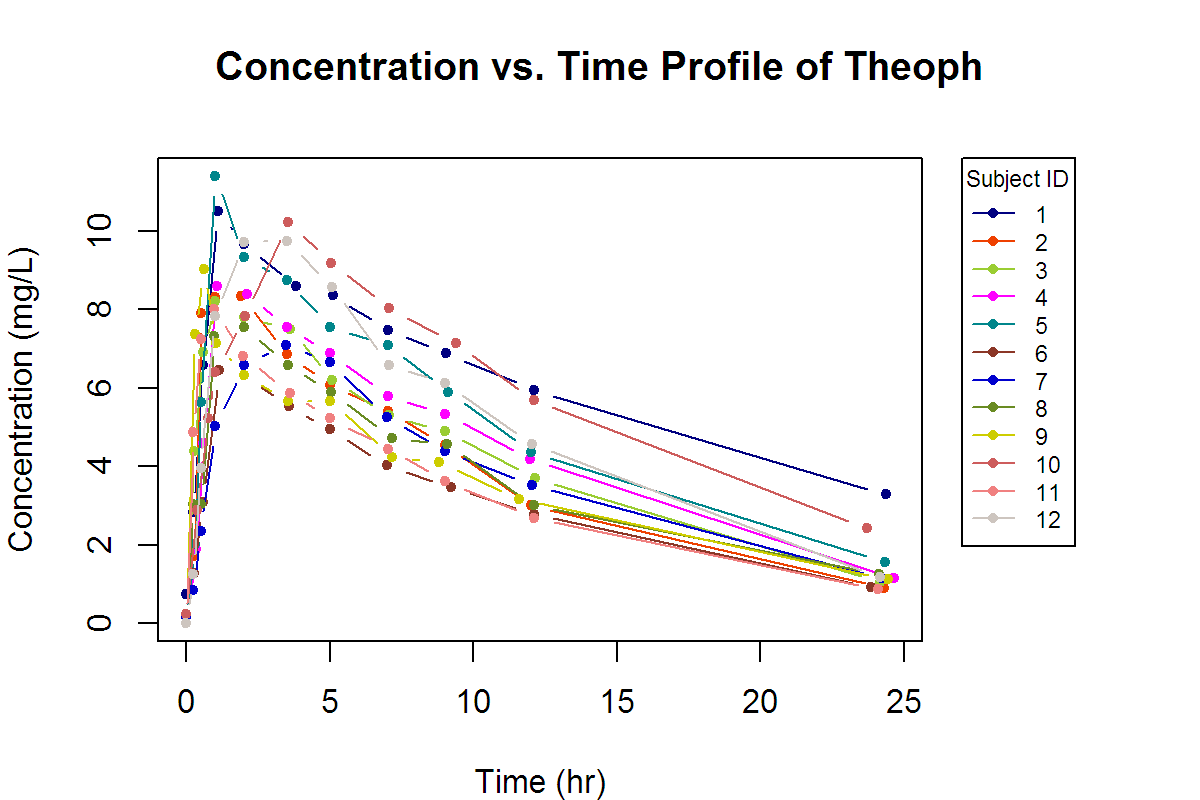
\includegraphics{Output/PK_Profile_Linear_Scale_for_Theoph.png}
\caption{\label{fig:unnamed-chunk-19}평균 약동학 파라메터와 그룹 농도-시간
그림 (선형)}
\end{figure}

\begin{figure}
\centering
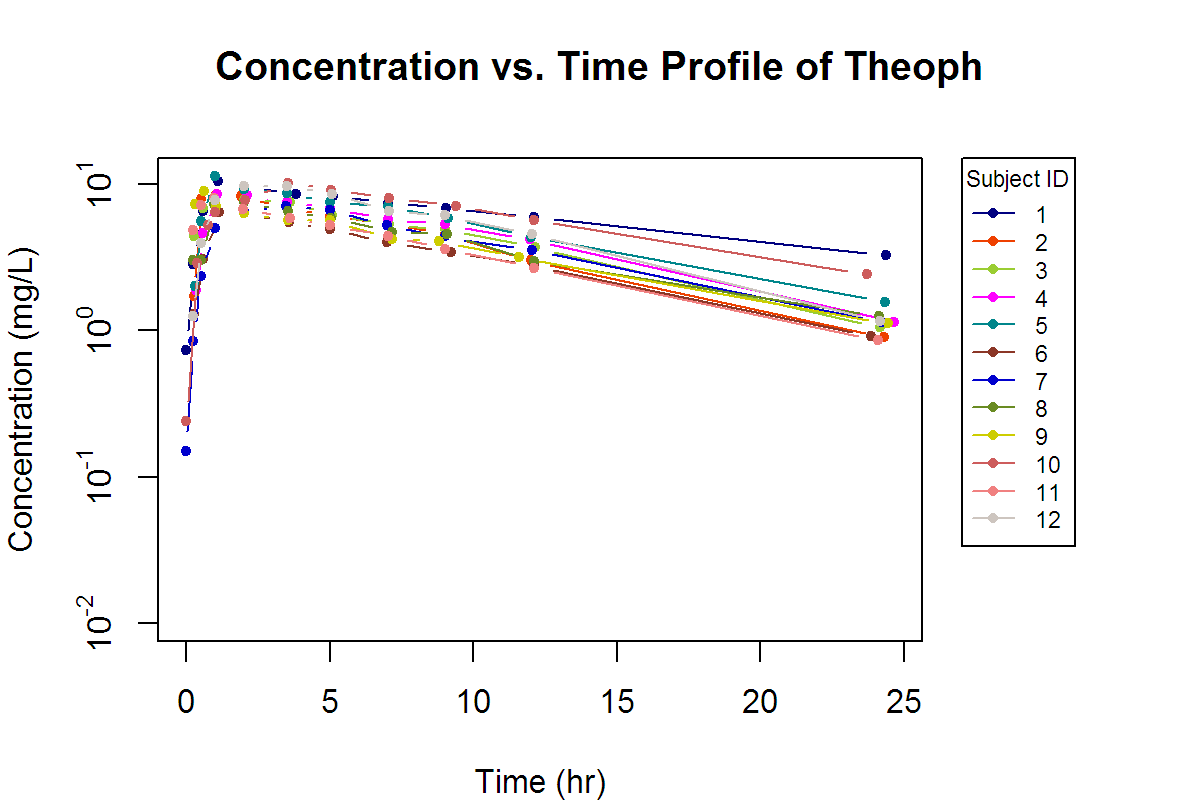
\includegraphics{Output/PK_Profile_Log_10_Scale_for_Theoph.png}
\caption{\label{fig:unnamed-chunk-20}평균 약동학 파라메터와 그룹 농도-시간
그림 (로그)}
\end{figure}

\begin{figure}
\centering
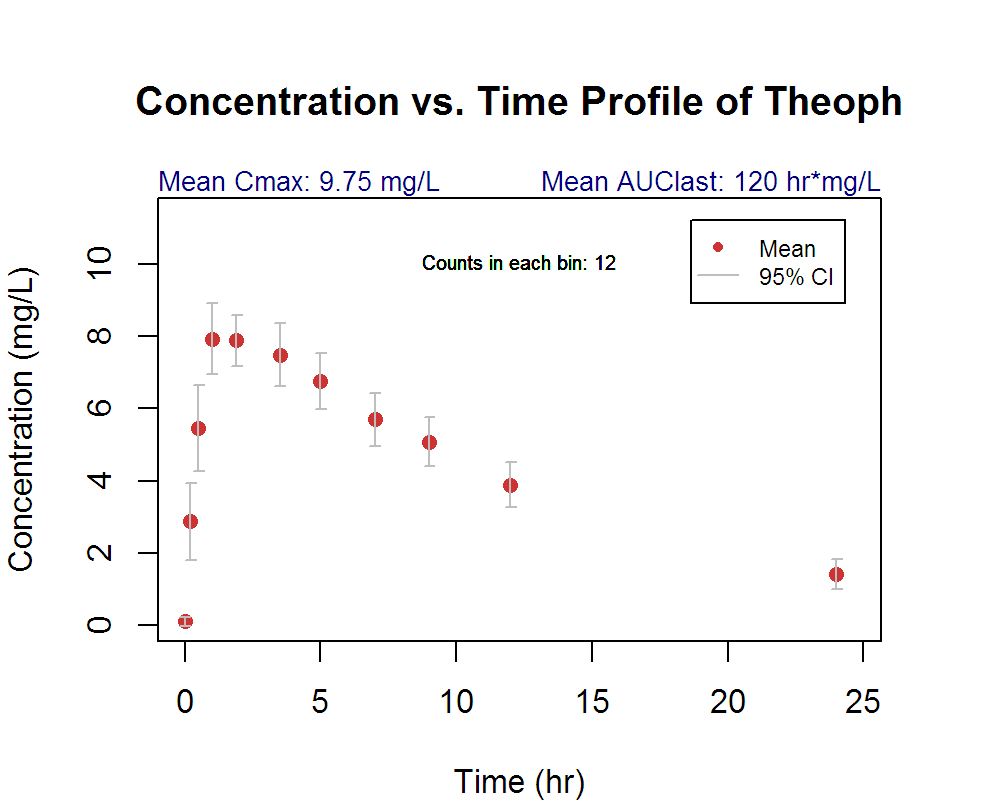
\includegraphics{Output/PK_Profile_with_CI_for_Theoph.png}
\caption{\label{fig:unnamed-chunk-21}평균 약동학 파라메터와 그룹 평균
농도-시간 그림 (로그)}
\end{figure}

또한 개개인 별로 여러개의 그림이 담긴 두개의 PDF 파일이 생성되었습니다.

\begin{itemize}
\tightlist
\item
  ./Output//Individual PK Linear Scale for Theoph.pdf
\item
  ./Output//Individual PK Log 10 Scale for Theoph.pdf
\end{itemize}

\begin{figure}
\centering
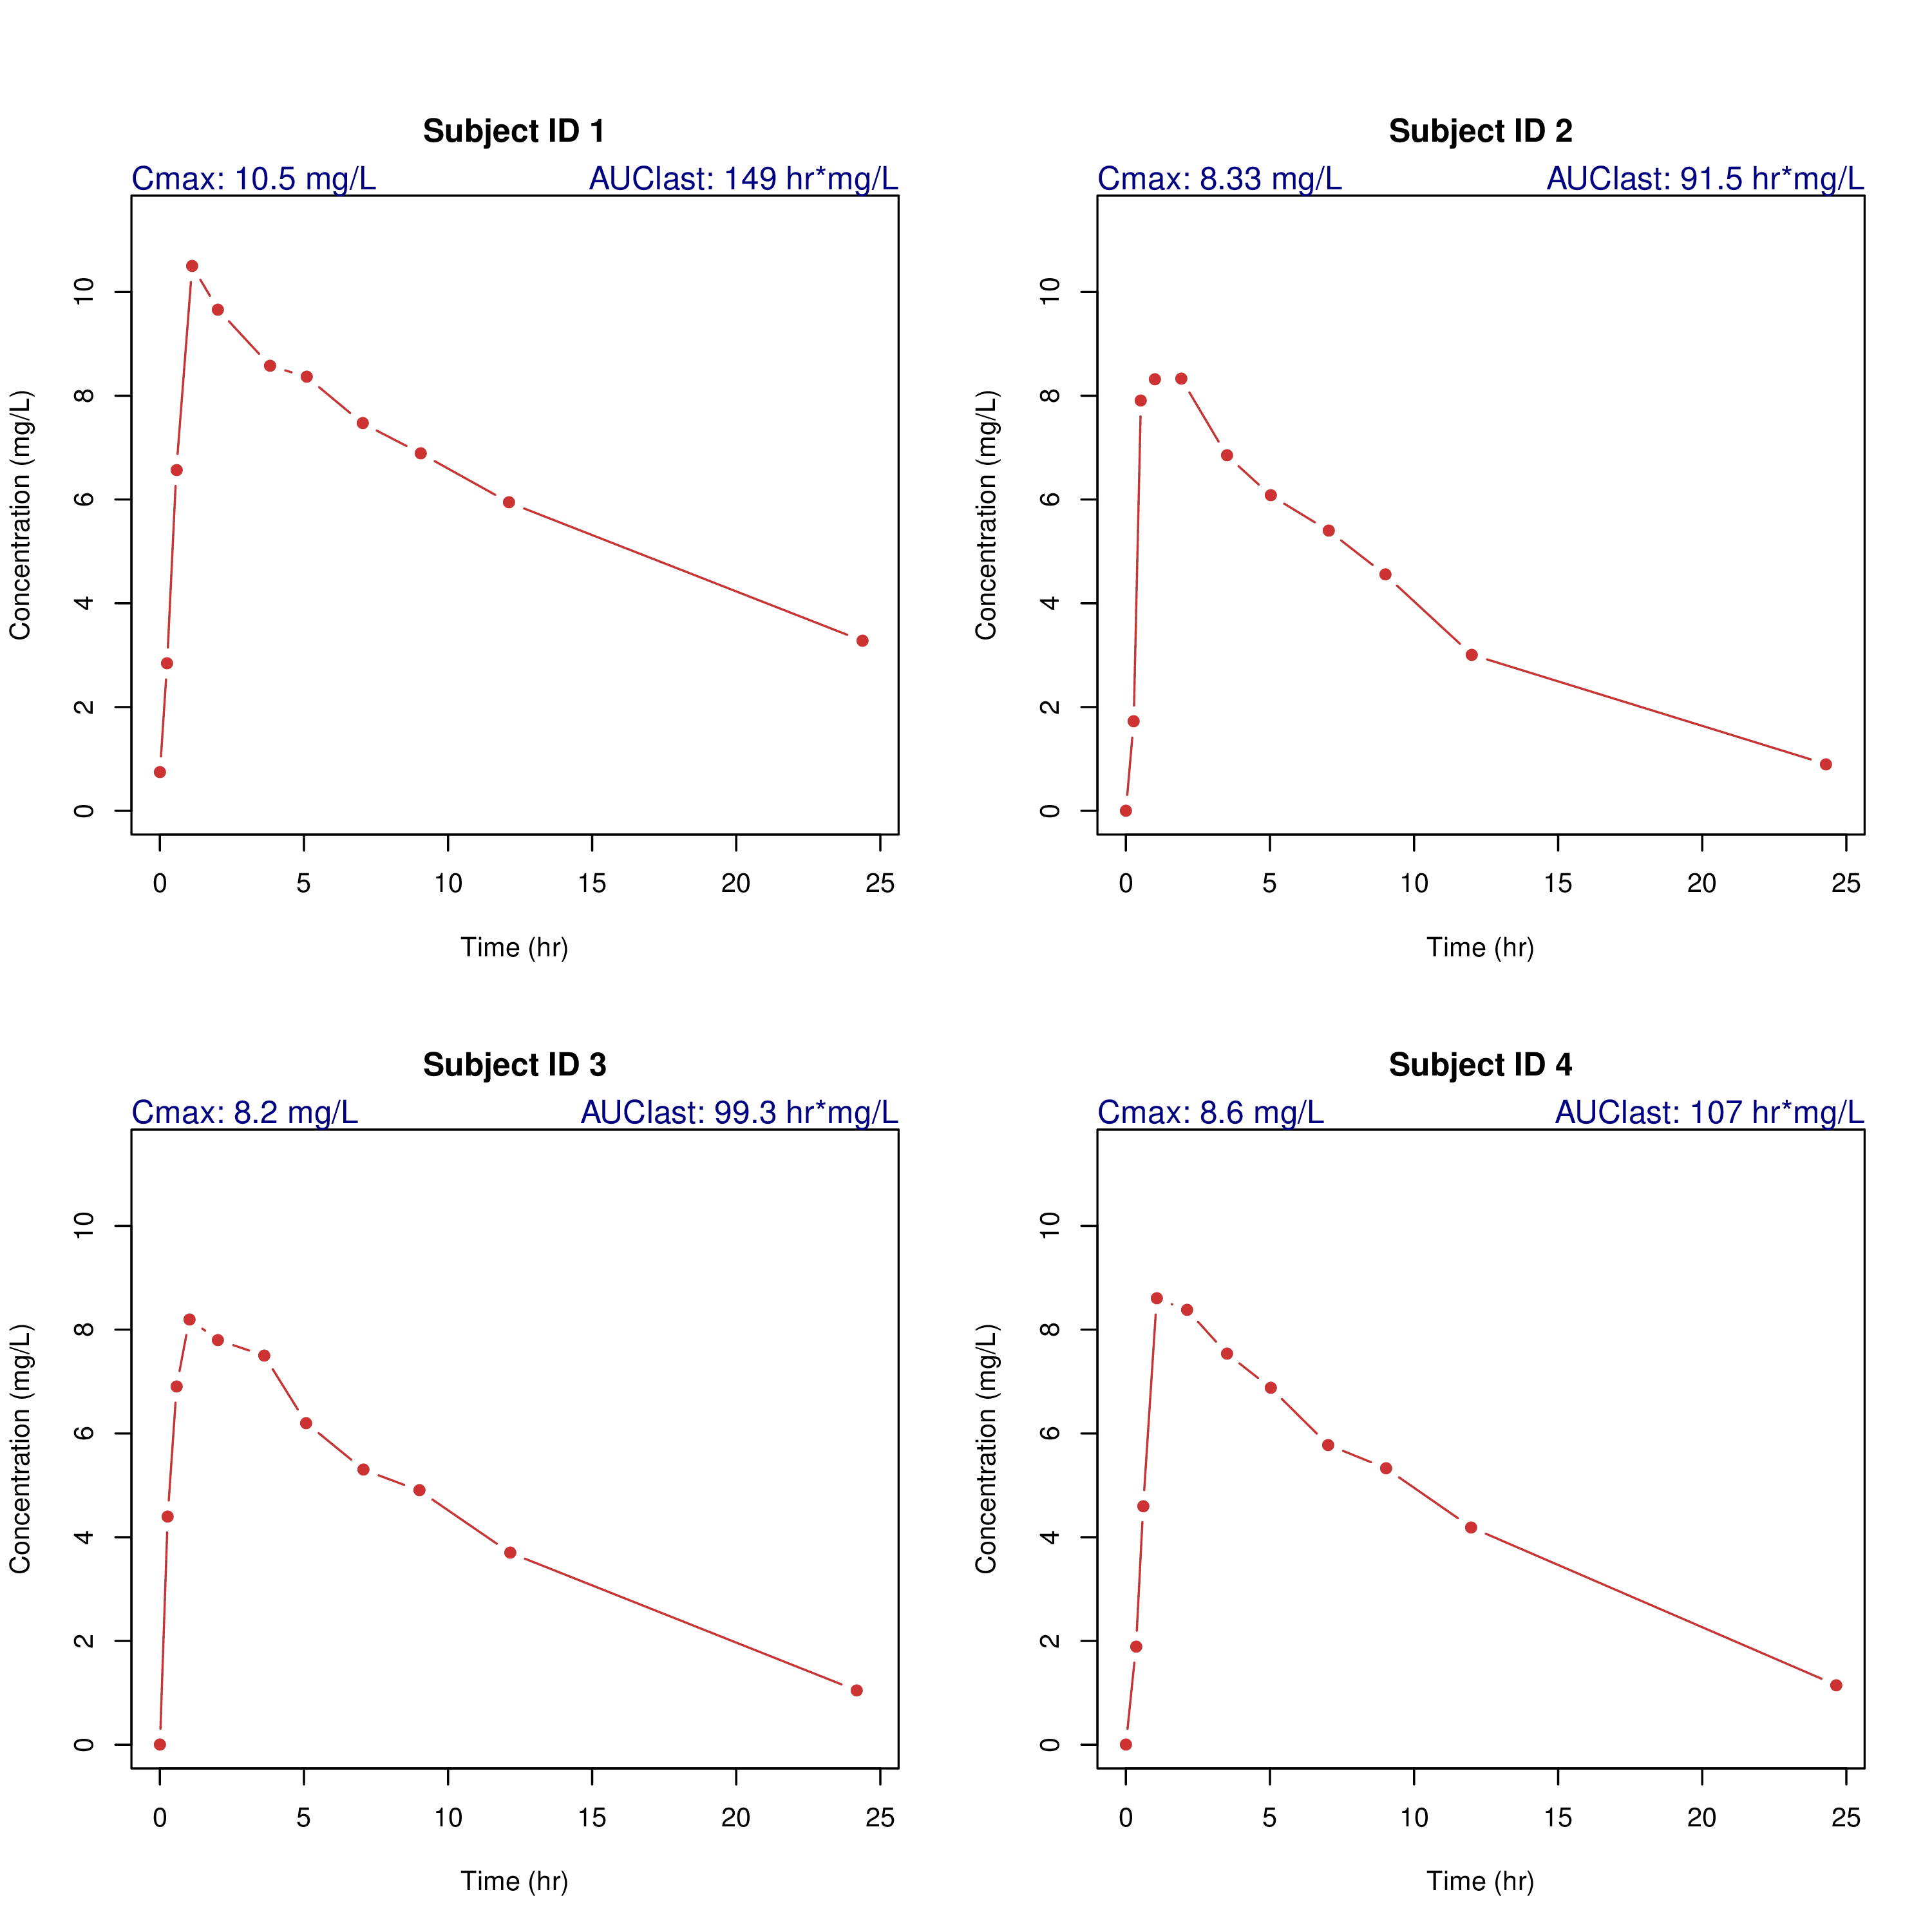
\includegraphics{Output/Individual_PK_Linear_Scale_for_Theoph00.png}
\caption{\label{fig:unnamed-chunk-22}약동학 파라메터와 함께 표시되는
농도-시간 그림 (선형)}
\end{figure}

\begin{figure}
\centering
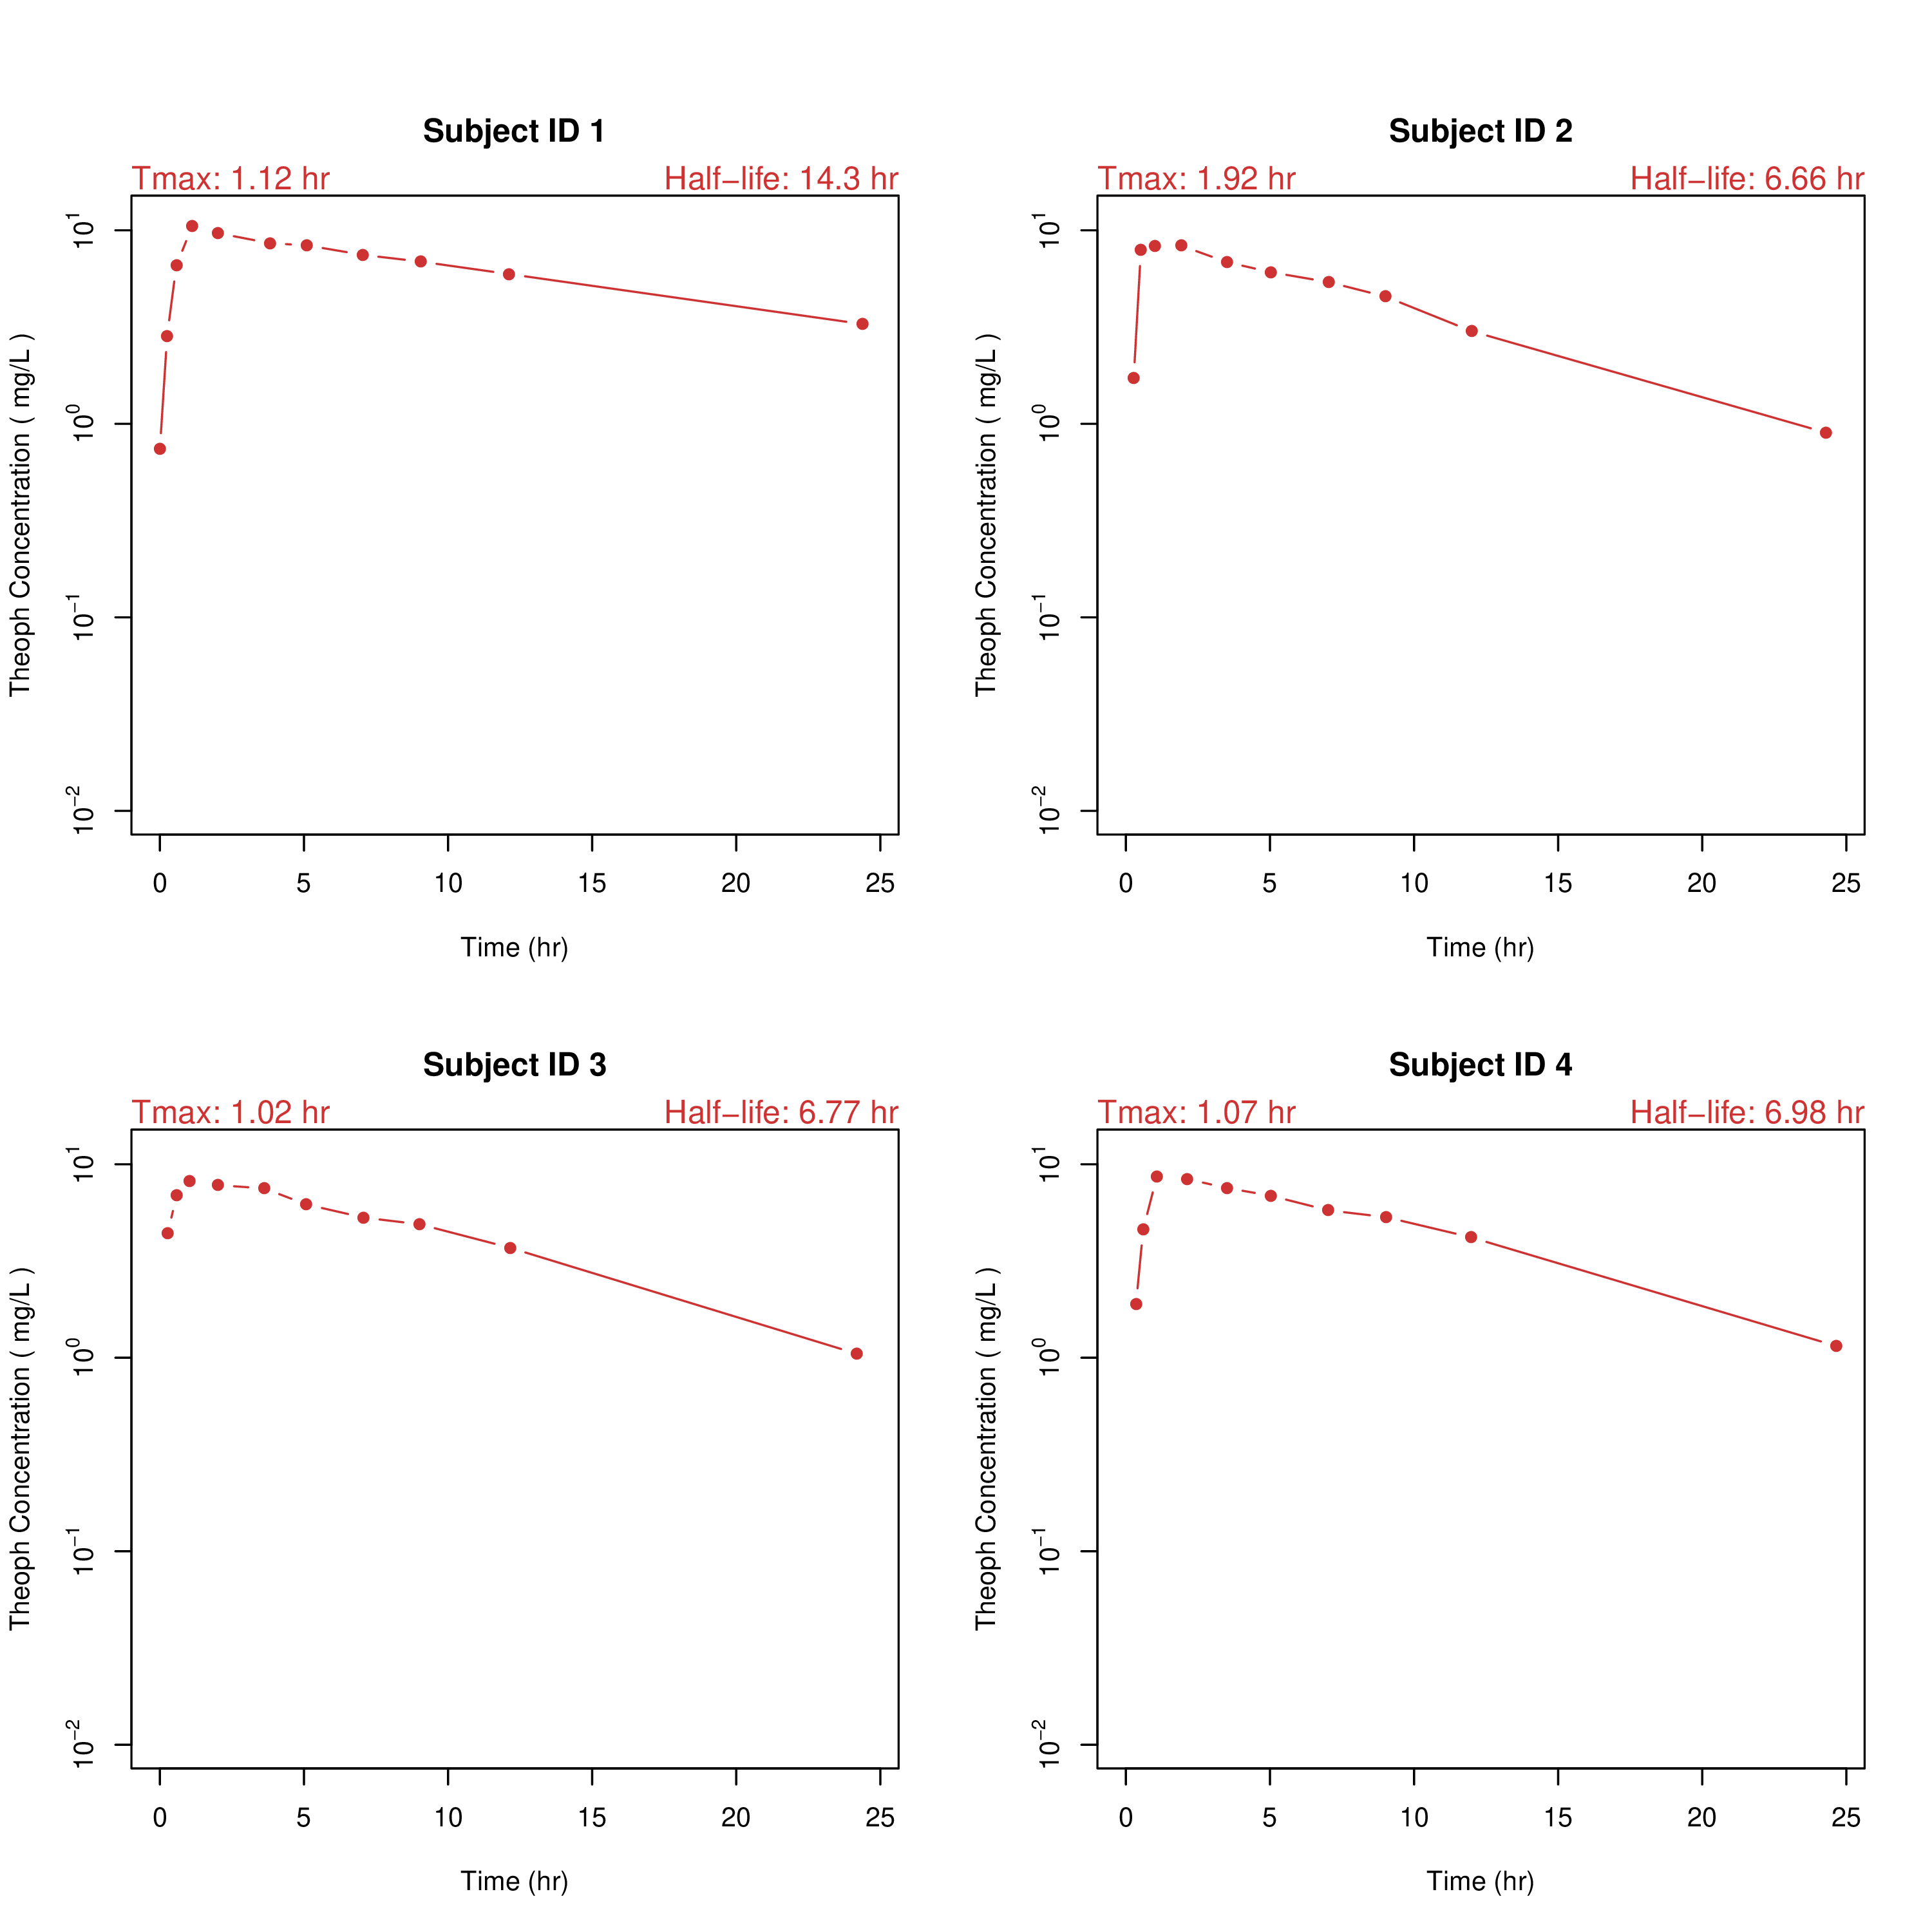
\includegraphics{Output/Individual_PK_Log_10_Scale_for_Theoph00.png}
\caption{\label{fig:unnamed-chunk-23}약동학 파라메터와 함께 표시되는
농도-시간 그림 (로그)}
\end{figure}

\chapter{R을 사용한 약동학 시뮬레이션}\label{simulation}

\section{이 장에서는}\label{summary-simulation}

\section{시뮬레이션에 대하여}\label{-}

TBD

\texttt{wnl} 패키지가 CRAN에 올라와 있습니다.

\section{시뮬레이션 후 비구획분석}\label{--}

TBD

\section{앱을 통해 살펴보는 시뮬레이션}\label{---}

샤이니 앱을 통해서 시뮬레이션을 구현할 수 있습니다. Shinyapp: PK
Simulation - 1 Comp IV or Oral \url{https://asan.shinyapps.io/pk1c/}

\begin{Shaded}
\begin{Highlighting}[]
\NormalTok{knitr}\OperatorTok{::}\KeywordTok{include_app}\NormalTok{(}\StringTok{"https://asan.shinyapps.io/pk1c/"}\NormalTok{) }\CommentTok{#, height = "600px")}
\end{Highlighting}
\end{Shaded}

\begin{verbatim}
## Error in (function (url = NULL, file = "webshot.png", vwidth = 992, vheight = 744, : webshot.js returned failure value: 1
\end{verbatim}

\subsection{shiny 앱}\label{shiny-}

웹브라우저를 통해 간단히 비구획분석을 할 수 있는 앱을 개발하였습니다.

\begin{itemize}
\tightlist
\item
  Han, S. (2017) pkrshiny: Noncompartmental Analysis using pkr R package
  Shiny application. URL: \url{https://asan.shinyapps.io/pkrshiny}
\end{itemize}

그 외 약동학과 관련된 몇가지 shiny 앱도 참고하세요.

\begin{itemize}
\tightlist
\item
  Han, S. (2017) Pharmacokinetic Simulation of one-compartment Models.
  URL: \url{https://asan.shinyapps.io/pk1c/}
\item
  Han, S. (2017) caff: Monte Carlo Simulation of Caffeine Shiny
  application. URL: \url{https://asan.shinyapps.io/caff}
\item
  Han, S. (2016) vtdm: Vancomycin TDM Shiny application. URL:
  \url{https://asan.shinyapps.io/vtdm}
\end{itemize}

\chapter{통계처리}\label{statistics}

\section{이 장에서는}\label{stat-intro}

생물학적 동등성, 용량 비례성을 확인하는 통계 처리 방법을 알아보겠습니다.

\begin{Shaded}
\begin{Highlighting}[]
\KeywordTok{library}\NormalTok{(tidyverse)}
\KeywordTok{library}\NormalTok{(ncarbe)}
\end{Highlighting}
\end{Shaded}

\begin{verbatim}
## Error in library(ncarbe): there is no package called 'ncarbe'
\end{verbatim}

\begin{Shaded}
\begin{Highlighting}[]
\KeywordTok{library}\NormalTok{(broom)}
\end{Highlighting}
\end{Shaded}

\section{기술통계량 구하기}\label{-}

앞서 \ref{noncompart}장에서 구한 \texttt{TheophNca}를 갖고 기술 통계량
(평균, 표준편차, 최소값, 최대값, skewness, kurtosis)을 구해보겠습니다.
\texttt{broom::tidy()} 함수를 사용하면 간단히 구할 수 있습니다. 다만
\texttt{NonCompart::tblNCA()} 후 \texttt{data.frame} 형태로 저장되어
입력으로 주어져야 합니다.

\begin{Shaded}
\begin{Highlighting}[]
\NormalTok{descStatTheophNca <-}\StringTok{ }\KeywordTok{tidy}\NormalTok{(}\KeywordTok{data.frame}\NormalTok{(TheophNca, }\DataTypeTok{stringsAsFactors =} \OtherTok{FALSE}\NormalTok{)) }\OperatorTok\StringTok{ }
\StringTok{  }\KeywordTok{select}\NormalTok{(column, n, mean, sd, min, max, skew, kurtosis)}

\NormalTok{knitr}\OperatorTok{::}\KeywordTok{kable}\NormalTok{(descStatTheophNca, }\DataTypeTok{digits =} \DecValTok{2}\NormalTok{)}
\end{Highlighting}
\end{Shaded}

\begin{tabular}{l|r|r|r|r|r|r|r}
\hline
column & n & mean & sd & min & max & skew & kurtosis\\
\hline
Subject* & 12 & 6.50 & 3.61 & 1.00 & 12.00 & 0.00 & -1.50\\
\hline
b0* & 12 & 2.39 & 0.25 & 2.03 & 2.82 & 0.13 & -1.38\\
\hline
CMAX* & 12 & 8.76 & 1.47 & 6.44 & 11.40 & 0.21 & -1.19\\
\hline
CMAXD* & 12 & 0.03 & 0.00 & 0.02 & 0.04 & 0.21 & -1.19\\
\hline
TMAX* & 12 & 1.79 & 1.11 & 0.63 & 3.55 & 0.70 & -1.35\\
\hline
TLAG* & 12 & 0.00 & 0.00 & 0.00 & 0.00 & NaN & NaN\\
\hline
CLST* & 12 & 1.40 & 0.72 & 0.86 & 3.28 & 1.57 & 1.14\\
\hline
CLSTP* & 12 & 1.40 & 0.72 & 0.86 & 3.28 & 1.58 & 1.19\\
\hline
TLST* & 12 & 24.20 & 0.25 & 23.70 & 24.65 & -0.28 & -0.57\\
\hline
LAMZHL* & 12 & 8.18 & 2.12 & 6.29 & 14.30 & 1.90 & 2.97\\
\hline
LAMZ* & 12 & 0.09 & 0.02 & 0.05 & 0.11 & -0.92 & 0.40\\
\hline
LAMZLL* & 12 & 7.49 & 2.40 & 2.03 & 9.38 & -1.20 & -0.03\\
\hline
LAMZUL* & 12 & 24.20 & 0.25 & 23.70 & 24.65 & -0.28 & -0.57\\
\hline
LAMZNPT* & 12 & 3.83 & 1.34 & 3.00 & 7.00 & 1.32 & 0.28\\
\hline
CORRXY* & 12 & -1.00 & 0.00 & -1.00 & -1.00 & 2.20 & 3.87\\
\hline
R2* & 12 & 1.00 & 0.00 & 0.99 & 1.00 & -2.20 & 3.87\\
\hline
R2ADJ* & 12 & 1.00 & 0.00 & 0.99 & 1.00 & -2.05 & 3.39\\
\hline
AUCLST* & 12 & 103.81 & 23.65 & 73.78 & 148.92 & 0.56 & -1.12\\
\hline
AUCALL* & 12 & 103.81 & 23.65 & 73.78 & 148.92 & 0.56 & -1.12\\
\hline
AUCIFO* & 12 & 122.19 & 38.13 & 84.25 & 216.61 & 1.25 & 0.51\\
\hline
AUCIFOD* & 12 & 0.38 & 0.12 & 0.26 & 0.68 & 1.25 & 0.51\\
\hline
AUCIFP* & 12 & 122.18 & 38.11 & 84.50 & 216.61 & 1.26 & 0.52\\
\hline
AUCIFPD* & 12 & 0.38 & 0.12 & 0.26 & 0.68 & 1.26 & 0.52\\
\hline
AUCPEO* & 12 & 13.54 & 6.35 & 8.13 & 31.25 & 1.71 & 2.19\\
\hline
AUCPEP* & 12 & 13.54 & 6.34 & 8.16 & 31.25 & 1.72 & 2.23\\
\hline
AUMCLST* & 12 & 883.06 & 262.98 & 609.15 & 1459.07 & 0.92 & -0.42\\
\hline
AUMCIFO* & 12 & 1590.30 & 1006.57 & 928.56 & 4505.53 & 2.00 & 2.96\\
\hline
AUMCIFP* & 12 & 1589.85 & 1006.06 & 928.49 & 4505.67 & 2.01 & 2.97\\
\hline
AUMCPEO* & 12 & 38.72 & 11.10 & 26.50 & 67.62 & 1.29 & 1.10\\
\hline
AUMCPEP* & 12 & 38.72 & 11.07 & 26.59 & 67.62 & 1.30 & 1.14\\
\hline
VZFO* & 12 & 31.93 & 6.47 & 22.22 & 43.26 & 0.20 & -1.40\\
\hline
VZFP* & 12 & 31.92 & 6.46 & 22.22 & 43.14 & 0.19 & -1.41\\
\hline
CLFO* & 12 & 2.81 & 0.68 & 1.48 & 3.80 & -0.45 & -0.93\\
\hline
CLFP* & 12 & 2.81 & 0.68 & 1.48 & 3.79 & -0.46 & -0.93\\
\hline
MRTEVLST* & 12 & 8.41 & 0.59 & 7.71 & 9.80 & 0.99 & 0.12\\
\hline
MRTEVIFO* & 12 & 12.29 & 2.96 & 9.98 & 20.80 & 1.90 & 2.83\\
\hline
MRTEVIFP* & 12 & 12.29 & 2.95 & 9.95 & 20.80 & 1.91 & 2.84\\
\hline
\end{tabular}

\section{생물학적 동등성}\label{bioequivalence}

생물학적 동등성을 위한 가장 간단한 방법은 \texttt{ncarbe}
패키지({\textbf{???}})를 쓰는 것입니다.\\
Chow와 Liu의 책의 내용을 충실히 반영하였습니다. (Chow
\protect\hyperlink{ref-chow2009design}{2009}) 현재로서는 2x2 디자인의
간단한 임상시험 디자인만을 지원하고 있습니다. (그림 \ref{fig:twobytwo})
핵심이 되는 함수는 \texttt{beNCA()} 입니다.

\begin{Shaded}
\begin{Highlighting}[]
\KeywordTok{include_graphics}\NormalTok{(}\StringTok{'assets/twobytwo.jpg'}\NormalTok{)}
\end{Highlighting}
\end{Shaded}

\begin{figure}
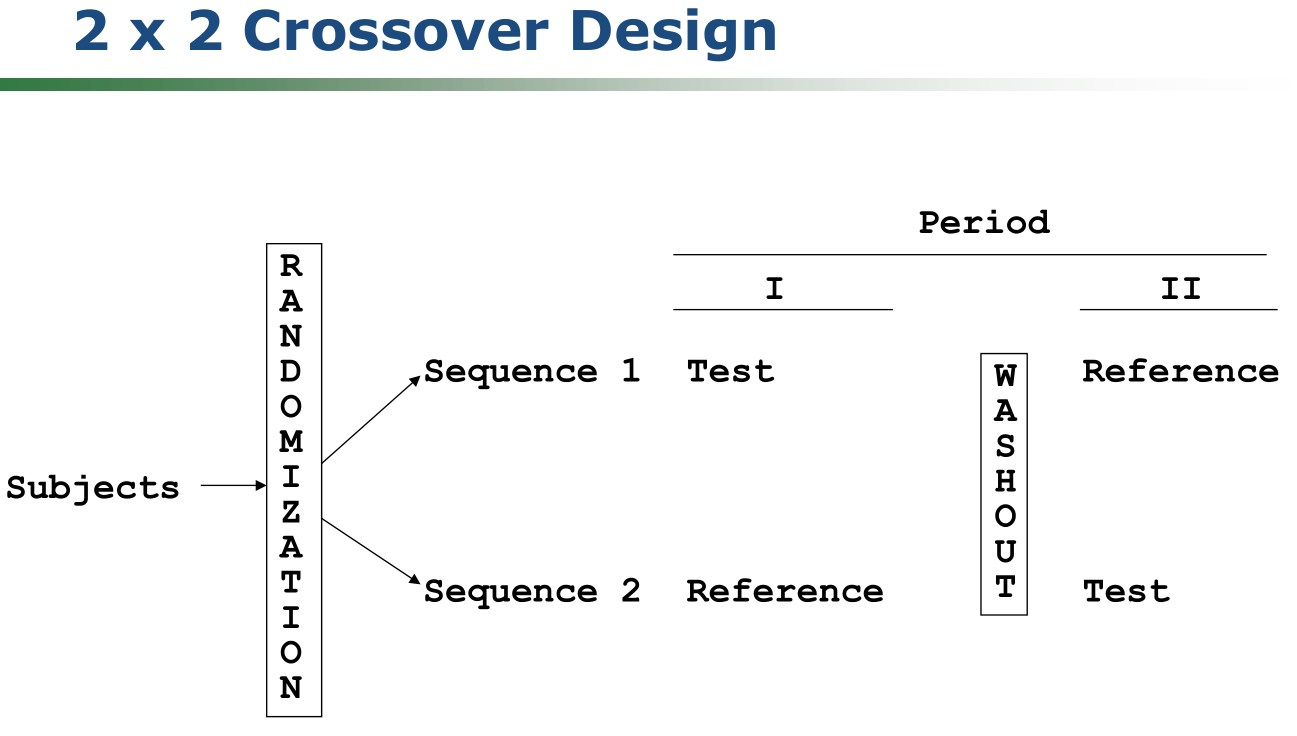
\includegraphics[width=18.01in]{assets/twobytwo} \caption{전형적인 2x2 설계}\label{fig:twobytwo}
\end{figure}

\begin{verbatim}
## Error in args(beNCA): 객체 'beNCA'를 찾을 수 없습니다
\end{verbatim}

다음과 같은 함수 인자를 설정해 주면 됩니다.

\begin{itemize}
\tightlist
\item
  SUBJ: Subject ID, any data type
\item
  GRP: column name in which information of ``RT'' or ``TR'' exists.
\item
  PRD: column name in which information of 1 or 2 exists.
\item
  TRT: column name in which information of ``R'' or ``T'' exists.
\item
  method: \texttt{kbe} by authors or \texttt{nlme} package uploaded on
  CRAN
\end{itemize}

\begin{Shaded}
\begin{Highlighting}[]
\NormalTok{file <-}\StringTok{ }\KeywordTok{system.file}\NormalTok{(}\StringTok{'example'}\NormalTok{, }\StringTok{'beConc.csv'}\NormalTok{, }\DataTypeTok{package =} \StringTok{'ncarbe'}\NormalTok{)}
\NormalTok{concData <-}\StringTok{ }\KeywordTok{read.csv}\NormalTok{(file, }\DataTypeTok{as.is =} \OtherTok{TRUE}\NormalTok{)}
\end{Highlighting}
\end{Shaded}

\begin{verbatim}
## Error in read.table(file = file, header = header, sep = sep, quote = quote, : no lines available in input
\end{verbatim}

\begin{Shaded}
\begin{Highlighting}[]
\KeywordTok{beNCA}\NormalTok{(concData)}
\end{Highlighting}
\end{Shaded}

\begin{verbatim}
## Error in beNCA(concData): 함수 "beNCA"를 찾을 수 없습니다
\end{verbatim}

배균섭 교수님의 강의 자료에서 가져왔습니다.

\begin{Shaded}
\begin{Highlighting}[]
\KeywordTok{include_graphics}\NormalTok{(}\StringTok{'assets/fixed-random.jpg'}\NormalTok{)}
\end{Highlighting}
\end{Shaded}

\begin{figure}
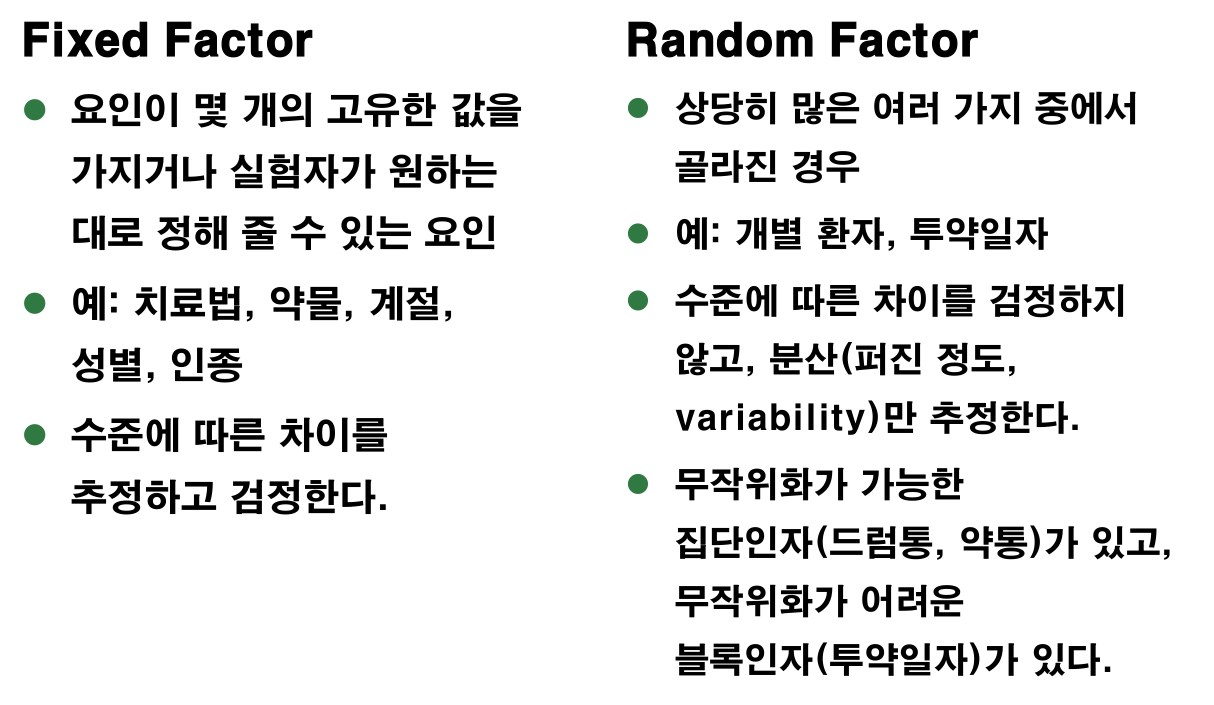
\includegraphics[width=16.86in]{assets/fixed-random} \caption{모수 인자와 변량 인자의 비교}\label{fig:fixedrandom}
\end{figure}

\section{Dose Proportionality}\label{dp}

DP 처리.

16명의 C\textsubscript{max}와 AUC\textsubscript{last}가 나온 표입니다.
Table \ref{tab:sad-pk}

\begin{Shaded}
\begin{Highlighting}[]
\CommentTok{# setup ----}

\KeywordTok{library}\NormalTok{(readxl)}
\KeywordTok{library}\NormalTok{(tidyverse)}
\KeywordTok{library}\NormalTok{(broom)}

\NormalTok{dp_data <-}\StringTok{ }\CommentTok{# Virtual data from 4 dose groups (N=16)}
\StringTok{'Dose,Subject,Cmax,AUClast}
\StringTok{50,101,860,2000}
\StringTok{50,102,510,2300}
\StringTok{50,103,620,2900}
\StringTok{50,104,540,2400}
\StringTok{100,201,1550,6600}
\StringTok{100,202,1440,7400}
\StringTok{100,203,2000,7300}
\StringTok{100,204,1600,7000}
\StringTok{200,301,4100,20400}
\StringTok{200,302,2800,9500}
\StringTok{200,303,3200,8000}
\StringTok{200,304,2550,7070}
\StringTok{400,401,4800,22000}
\StringTok{400,402,5700,23000}
\StringTok{400,403,5800,26700}
\StringTok{400,404,5760,28884'}

\NormalTok{sad_indi_pk <-}\StringTok{ }\KeywordTok{read_csv}\NormalTok{(dp_data)}
\KeywordTok{kable}\NormalTok{(sad_indi_pk, }\DataTypeTok{caption =} \StringTok{'16명의 C~max~, AUC~last~'}\NormalTok{)}
\end{Highlighting}
\end{Shaded}

\begin{table}

\caption{\label{tab:sad-pk}16명의 C~max~, AUC~last~}
\centering
\begin{tabular}[t]{r|r|r|r}
\hline
Dose & Subject & Cmax & AUClast\\
\hline
50 & 101 & 860 & 2000\\
\hline
50 & 102 & 510 & 2300\\
\hline
50 & 103 & 620 & 2900\\
\hline
50 & 104 & 540 & 2400\\
\hline
100 & 201 & 1550 & 6600\\
\hline
100 & 202 & 1440 & 7400\\
\hline
100 & 203 & 2000 & 7300\\
\hline
100 & 204 & 1600 & 7000\\
\hline
200 & 301 & 4100 & 20400\\
\hline
200 & 302 & 2800 & 9500\\
\hline
200 & 303 & 3200 & 8000\\
\hline
200 & 304 & 2550 & 7070\\
\hline
400 & 401 & 4800 & 22000\\
\hline
400 & 402 & 5700 & 23000\\
\hline
400 & 403 & 5800 & 26700\\
\hline
400 & 404 & 5760 & 28884\\
\hline
\end{tabular}
\end{table}

그림을 살펴보겠습니다.

\begin{Shaded}
\begin{Highlighting}[]
\NormalTok{sad_indi_pk_log <-}\StringTok{ }\NormalTok{sad_indi_pk }\OperatorTok\StringTok{ }\KeywordTok{mutate_all}\NormalTok{(log)}

\NormalTok{figA <-}\StringTok{ }\KeywordTok{ggplot}\NormalTok{(sad_indi_pk_log, }\KeywordTok{aes}\NormalTok{(}\DataTypeTok{x=}\NormalTok{Dose, }\DataTypeTok{y=}\NormalTok{Cmax)) }\OperatorTok{+}
\StringTok{  }\KeywordTok{geom_smooth}\NormalTok{(}\DataTypeTok{method =} \StringTok{'lm'}\NormalTok{)}\OperatorTok{+}
\StringTok{  }\KeywordTok{geom_boxplot}\NormalTok{(}\KeywordTok{aes}\NormalTok{(}\DataTypeTok{group =}\NormalTok{ Dose), }
               \DataTypeTok{size =} \DecValTok{1}\NormalTok{, }
               \DataTypeTok{outlier.colour =} \StringTok{"red"}\NormalTok{, }
               \DataTypeTok{outlier.shape =} \DecValTok{1}\NormalTok{, }
               \DataTypeTok{outlier.size =} \DecValTok{3}\NormalTok{) }\OperatorTok{+}
\StringTok{  }\KeywordTok{theme_bw}\NormalTok{() }\OperatorTok{+}
\StringTok{  }\KeywordTok{scale_x_continuous}\NormalTok{(}\DataTypeTok{breaks =} \KeywordTok{c}\NormalTok{(}\DecValTok{50}\NormalTok{, }\DecValTok{100}\NormalTok{, }\DecValTok{200}\NormalTok{, }\DecValTok{400}\NormalTok{)) }\OperatorTok{+}
\StringTok{  }\KeywordTok{labs}\NormalTok{(}\DataTypeTok{x =} \StringTok{'Dose (mg)'}\NormalTok{, }\DataTypeTok{y =} \KeywordTok{expression}\NormalTok{(}\StringTok{'C'}\NormalTok{[max]}\OperatorTok{*}\StringTok{' (ng/mL)'}\NormalTok{),}
       \DataTypeTok{title =} \KeywordTok{expression}\NormalTok{(}\StringTok{'C'}\NormalTok{[max]))}
\NormalTok{figA}
\end{Highlighting}
\end{Shaded}

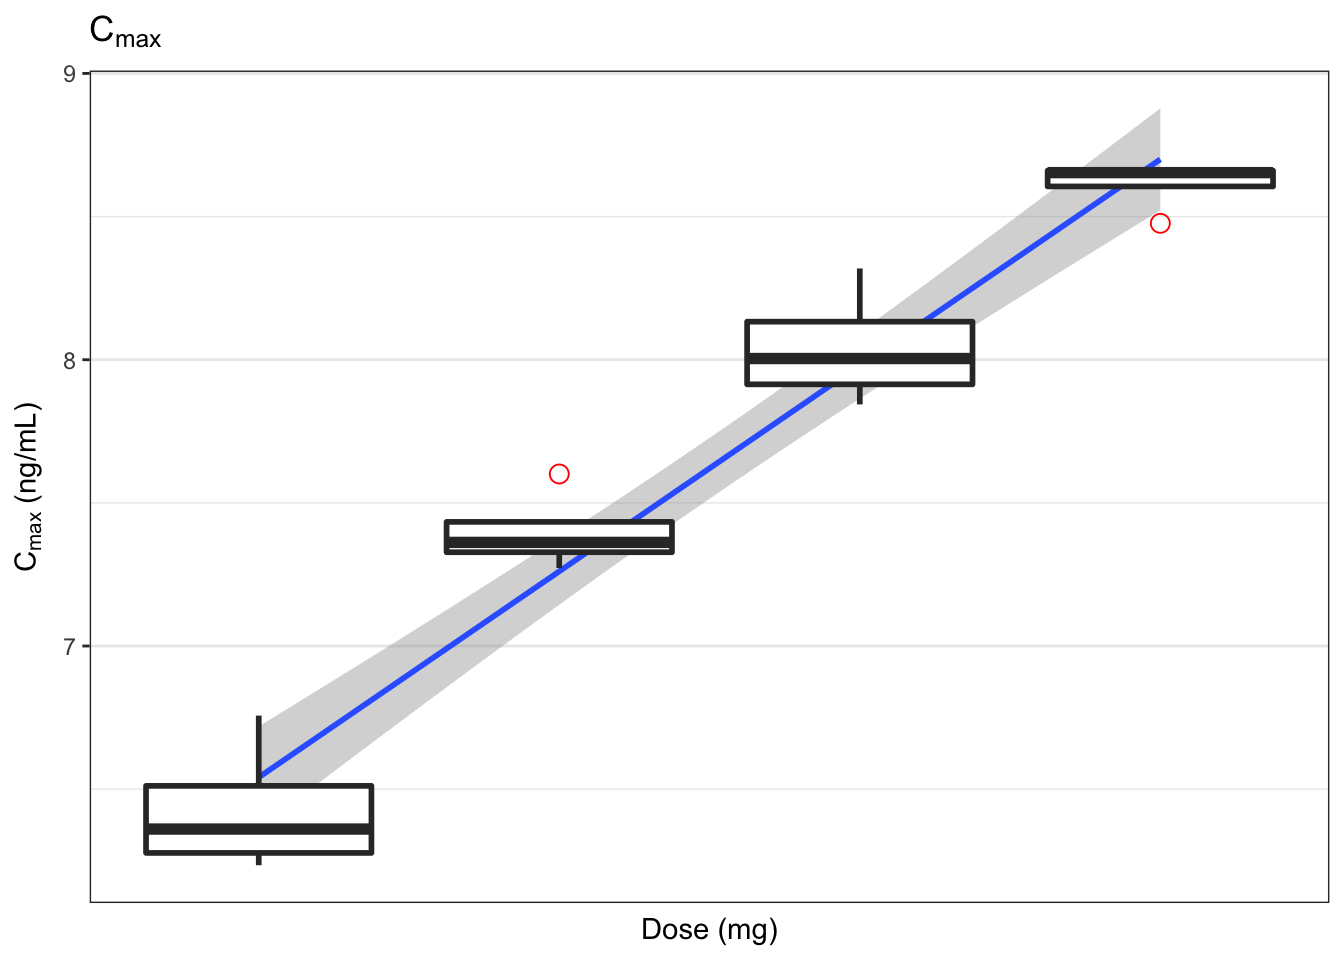
\includegraphics{book-ncar_files/figure-latex/unnamed-chunk-29-1.pdf}

\begin{Shaded}
\begin{Highlighting}[]
\NormalTok{figB <-}\StringTok{ }\KeywordTok{ggplot}\NormalTok{(sad_indi_pk_log, }\KeywordTok{aes}\NormalTok{(}\DataTypeTok{x=}\NormalTok{Dose, }\DataTypeTok{y=}\NormalTok{AUClast)) }\OperatorTok{+}
\StringTok{  }\KeywordTok{geom_smooth}\NormalTok{(}\DataTypeTok{method =} \StringTok{'lm'}\NormalTok{)}\OperatorTok{+}
\StringTok{  }\KeywordTok{geom_boxplot}\NormalTok{(}\KeywordTok{aes}\NormalTok{(}\DataTypeTok{group =}\NormalTok{ Dose), }
               \DataTypeTok{size =} \DecValTok{1}\NormalTok{, }
               \DataTypeTok{outlier.colour =} \StringTok{"red"}\NormalTok{, }
               \DataTypeTok{outlier.shape =} \DecValTok{1}\NormalTok{, }
               \DataTypeTok{outlier.size =} \DecValTok{3}\NormalTok{) }\OperatorTok{+}
\StringTok{  }\KeywordTok{theme_bw}\NormalTok{() }\OperatorTok{+}
\StringTok{  }\KeywordTok{scale_x_continuous}\NormalTok{(}\DataTypeTok{breaks =} \KeywordTok{c}\NormalTok{(}\DecValTok{50}\NormalTok{, }\DecValTok{100}\NormalTok{, }\DecValTok{200}\NormalTok{, }\DecValTok{400}\NormalTok{)) }\OperatorTok{+}
\StringTok{  }\KeywordTok{labs}\NormalTok{(}\DataTypeTok{x =} \StringTok{'Dose (mg)'}\NormalTok{, }\DataTypeTok{y =} \KeywordTok{expression}\NormalTok{(}\StringTok{'AUC'}\NormalTok{[(}\DecValTok{0}\OperatorTok{-}\NormalTok{last)]}\OperatorTok{*}\StringTok{' (ng·hr/mL)'}\NormalTok{),}
       \DataTypeTok{title =} \KeywordTok{expression}\NormalTok{(}\StringTok{'AUC'}\NormalTok{[(}\DecValTok{0}\OperatorTok{-}\NormalTok{last)]))}
\NormalTok{figB}
\end{Highlighting}
\end{Shaded}

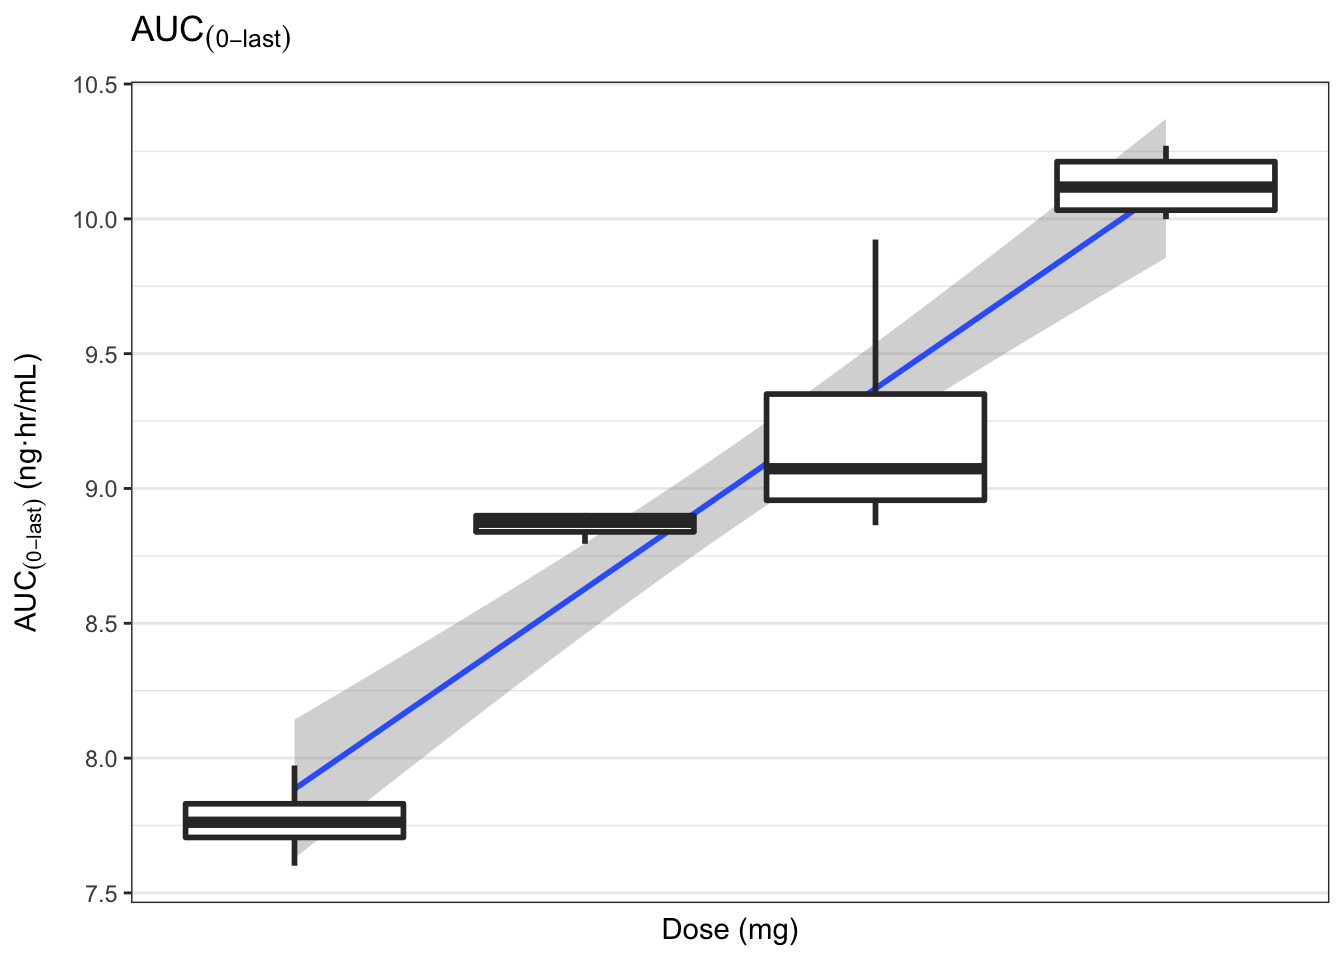
\includegraphics{book-ncar_files/figure-latex/unnamed-chunk-29-2.pdf}

lm() 함수를 써서 구할 수 있습니다.

\begin{Shaded}
\begin{Highlighting}[]
\NormalTok{calc_dp <-}\StringTok{ }\ControlFlowTok{function}\NormalTok{(param, fit) \{}
  \KeywordTok{bind_cols}\NormalTok{(fit }\OperatorTok\StringTok{ }\NormalTok{summary }\OperatorTok\StringTok{ }\NormalTok{tidy }\OperatorTok\StringTok{ }\KeywordTok{filter}\NormalTok{(term }\OperatorTok{==}\StringTok{ 'Dose'}\NormalTok{), }
\NormalTok{            fit }\OperatorTok\StringTok{ }\KeywordTok{confint}\NormalTok{(}\DataTypeTok{level =} \FloatTok{0.95}\NormalTok{) }\OperatorTok\StringTok{ }\NormalTok{tidy }\OperatorTok\StringTok{ }\KeywordTok{filter}\NormalTok{(.rownames }\OperatorTok{==}\StringTok{ 'Dose'}\NormalTok{), }
\NormalTok{            fit }\OperatorTok\StringTok{ }\NormalTok{summary }\OperatorTok\StringTok{ }\NormalTok{glance) }\OperatorTok\StringTok{ }
\StringTok{    }\KeywordTok{filter}\NormalTok{(term }\OperatorTok{==}\StringTok{ 'Dose'}\NormalTok{) }\OperatorTok\StringTok{ }
\StringTok{    }\KeywordTok{select}\NormalTok{(}\OperatorTok{-}\NormalTok{.rownames, }\OperatorTok{-}\NormalTok{term) }\OperatorTok\StringTok{ }
\StringTok{    }\KeywordTok{mutate}\NormalTok{(}\DataTypeTok{parameters =}\NormalTok{ param) }\OperatorTok\StringTok{ }
\StringTok{    }\KeywordTok{mutate}\NormalTok{(}\DataTypeTok{est =} \KeywordTok{sprintf}\NormalTok{(}\StringTok{'%0.2f (%0.2f)'}\NormalTok{, estimate, std.error)) }\OperatorTok\StringTok{ }
\StringTok{    }\KeywordTok{mutate}\NormalTok{(}\DataTypeTok{ci =} \KeywordTok{sprintf}\NormalTok{(}\StringTok{'%0.2f-%0.2f'}\NormalTok{, X2.}\DecValTok{5}\NormalTok{.., X97.}\DecValTok{5}\NormalTok{..)) }\OperatorTok\StringTok{ }
\StringTok{    }\KeywordTok{select}\NormalTok{(parameters, est, ci, r.squared, p.value)}
\NormalTok{\}}

\NormalTok{fit_cmax <-}\StringTok{ }\KeywordTok{lm}\NormalTok{(}\DataTypeTok{formula =}\NormalTok{ Cmax }\OperatorTok{~}\StringTok{ }\NormalTok{Dose, }\DataTypeTok{data =}\NormalTok{ sad_indi_pk_log)}
\NormalTok{fit_auclast <-}\StringTok{ }\KeywordTok{lm}\NormalTok{(}\DataTypeTok{formula =}\NormalTok{ AUClast }\OperatorTok{~}\StringTok{ }\NormalTok{Dose, }\DataTypeTok{data =}\NormalTok{ sad_indi_pk_log)}

\KeywordTok{bind_rows}\NormalTok{(}\KeywordTok{calc_dp}\NormalTok{(}\DataTypeTok{param =} \StringTok{'Cmax'}\NormalTok{, }\DataTypeTok{fit =}\NormalTok{ fit_cmax),}
          \KeywordTok{calc_dp}\NormalTok{(}\DataTypeTok{param =} \StringTok{'AUClast'}\NormalTok{, }\DataTypeTok{fit =}\NormalTok{ fit_auclast))}
\end{Highlighting}
\end{Shaded}

\begin{verbatim}
##   parameters         est        ci r.squared      p.value
## 1       Cmax 1.04 (0.06) 0.90-1.18 0.9494890 1.797428e-10
## 2    AUClast 1.07 (0.09) 0.87-1.27 0.9053706 1.486278e-08
\end{verbatim}

C\textsubscript{max}는 생동 기준을 만족하는데 반해
AUC\textsubscript{last}는 만족하지 않는 것을 알 수 있습니다.

\chapter{결과 및 논의}\label{result}

R을 통해서 NCA 를 구할 수 있도록 R 패키지를 구축하였습니다. 값비싼
상용소프트웨어를 사용하지 않고도 동일한 비구획분석이 가능한 것은 비용과
작업 효율 측면에서 큰 잇점을 가져올 것입니다.

현재 R에 기본적으로 내장되어 있는 PO 테오필린(theophylline)과 IV bolus
인도메타신(indomethacin)에 대해서 예가 잘 나와있습니다. 약물에 대한
자료를 고른 후 각 약물의 복용량, 감소 구간에서의 log 치환 여부,
복용방법, 정맥주사일 경우 투입 시간(정맥주사 이외의 값들 경우에는
infusion time은 내부 함수에 따라 값이 적용되지 않는다.)을 각각 설정할
경우 값을 도출할 수 있습니다.

Edison 내에서 실제 Theophylline의 용량에 따라 구현된 각각의 graph를
spaghetti plot형태로 Edison의 결과 가시화 tab을 이용하여 확인할 수
있으며, 그래프의 형태를 변형할 수 있게 설정하였다. Y축(농도)의 경우
linear plot과 semi-logarithmic plot을 모두 함께 확인할 수 있도록 하여
다양한 구간에서의 그래프의 추세를 선택적으로 확인할 수 있도록 하였다.

언급하였던 공식 이외에도 Pharmacokinetic and Pharmacodynamic Data
Analysis 5th edition 에 언급된 공식을 적용하여 다음과 같이 값을
도출하였다.(figure 8)

또한 결과 값이 모두 도출된 이후 실제 NCA program으로 가장 흔히 사용되고
있는 WinNonlin® (Version 7.0 Pharsight, CA, USA) software 와의 결과
비교에서도 모든 조건을 현재 Edison simulator에서 준 값과 동일하게
설정하여 프로그램을 실행할 경우, 모든 지표에서 같은 값이 계산됨을
확인하였다. (figure 8, figure 9)

현재 가장 간단한 분석 방식인 비구획 분석을 통해서 약동학 분석에 필수적인
지표들을 산출해 내었지만, 마찬가지로 수학적 원리를 반영하여 R script를
구성한다면 보다 고차원적적 약동학 분석 방법인 구획 분석(Compartmental
analysis)과 비선형적 약동학(nonlinear mixed effect modeling) 분석 또한
실시할 수 있다.

실제로 Edison 사이언스 엡에 추가한 `NONMEM(Nonlinear mixed effect
modeling), method'라는 엡을 통해 현재 입력 되어있는
Theoph(theophylline)의 시간 농도 데이터를 가지고 FO(first-order method),
FOCE(first-order conditional estimation method), LAPL(Laplace's
method)의 방법을 이용하여 현재 사용하는 NONMEM software와 유사한 값들을
재현해 낼 수 있다.

Figure 4 논문 내에서의 설정 값

Figure 5. 앞서 설정한 Theophylline에 대한 linear spaghetti plot

Figure 6. 앞서 설정한 Theophylline에 대한 scatter plot

Figure 7. 앞서 설정한 Theophylline에 대한 semi-logarithmic spaghetti
plot

Figure 8. 앞서 설정한 Theophylline에 대한 NCA 분석 결과

Figure 9. Theophylline에 대하여 같은 data와 설정값으로 계산한 WinNonlin®
(Version 7.0 Pharsight, CA, USA) software의 결과

Figure 10. NONMEM(Nonlinear mixed effect modeling), method 엡에 입력되어
있는 theophylline data의 농도 시간 곡선

Figure 11. theophylline data에 대한 model

Figure 12. nonlinear mixed effect modeling First order method를 통해
도출된 parameter

\chapter{결론}\label{conclusion}

약물을 연구하고 개발하는데 있어서 약동학은 굉장히 필수적인 분야이며, 그
동안 이러한 약동학 지표들을 구하기 위해서 그러한 결론이 도출되는 과정을
고려하지 않고 일부 프로그램의 사용에만 의존하는 모습이 주를 이뤘습니다.

하지만 이번 Edison program과 다양한 수학적, 통계적 지식을 coding에
활용하여 실제 임상적으로도 활용 가능한 결과값을 도출해 낼 수 있음을
확인하였으며 앞으로도 약동학 분야에서 다양하게 활용할 수 있을 것으로
예측됩니다.

\appendix \addcontentsline{toc}{chapter}{\appendixname}


\chapter{지원}

패키지와 관련한 모든 의문은
\href{mailto:shan@acp.kr}{\nolinkurl{shan@acp.kr}} / 02-3010-4614 으로
연락 주시면 빠르게 도움 드리겠습니다. 혹은 StackOverflow\footnote{\url{https://stackoverflow.com}}에
영어로 질문 올려주시고 링크를 보내주시면 더 좋습니다.

\chapter*{sessionInfo}\label{sessioninfo}


\begin{Shaded}
\begin{Highlighting}[]
\KeywordTok{sessionInfo}\NormalTok{()}
\end{Highlighting}
\end{Shaded}

\begin{verbatim}
## R version 3.4.2 (2017-09-28)
## Platform: x86_64-apple-darwin17.0.0 (64-bit)
## Running under: macOS High Sierra 10.13
## 
## Matrix products: default
## BLAS: /System/Library/Frameworks/Accelerate.framework/Versions/A/Frameworks/vecLib.framework/Versions/A/libBLAS.dylib
## LAPACK: /System/Library/Frameworks/Accelerate.framework/Versions/A/Frameworks/vecLib.framework/Versions/A/libLAPACK.dylib
## 
## locale:
## [1] ko_KR.UTF-8/ko_KR.UTF-8/ko_KR.UTF-8/C/ko_KR.UTF-8/ko_KR.UTF-8
## 
## attached base packages:
## [1] grid      stats     graphics  grDevices utils     datasets  base     
## 
## other attached packages:
##  [1] readxl_1.0.0         broom_0.4.2          bindrcpp_0.2        
##  [4] ncar_0.3.7           rtf_0.4-11           pkr_0.1.1           
##  [7] forestplot_1.7.2     checkmate_1.8.4      magrittr_1.5        
## [10] binr_1.1             foreign_0.8-69       NonCompart_0.3.3    
## [13] cowplot_0.8.0        knitr_1.17           forcats_0.2.0       
## [16] stringr_1.2.0        dplyr_0.7.4          purrr_0.2.4         
## [19] readr_1.1.1          tidyr_0.7.2          tibble_1.3.4        
## [22] ggplot2_2.2.1        tidyverse_1.1.1.9000
## 
## loaded via a namespace (and not attached):
##  [1] Rcpp_0.12.13      lubridate_1.6.0   lattice_0.20-35  
##  [4] png_0.1-7         clisymbols_1.2.0  assertthat_0.2.0 
##  [7] rprojroot_1.2     digest_0.6.12     psych_1.7.8      
## [10] R6_2.2.2          cellranger_1.1.0  plyr_1.8.4       
## [13] backports_1.1.1   evaluate_0.10.1   httr_1.3.1       
## [16] highr_0.6         rlang_0.1.2       lazyeval_0.2.0   
## [19] rstudioapi_0.7    R.oo_1.21.0       rmarkdown_1.6    
## [22] labeling_0.3      boxes_0.0.0.9000  webshot_0.4.2    
## [25] munsell_0.4.3     compiler_3.4.2    modelr_0.1.1     
## [28] pkgconfig_2.0.1   mnormt_1.5-5      htmltools_0.3.6  
## [31] tidyselect_0.2.2  bookdown_0.5      codetools_0.2-15 
## [34] crayon_1.3.4      R.methodsS3_1.7.1 nlme_3.1-131     
## [37] jsonlite_1.5      gtable_0.2.0      scales_0.5.0     
## [40] stringi_1.1.5     reshape2_1.4.2    xml2_1.1.1       
## [43] tools_3.4.2       glue_1.1.1        jpeg_0.1-8       
## [46] hms_0.3           parallel_3.4.2    yaml_2.1.14      
## [49] colorspace_1.3-2  rvest_0.3.2       bindr_0.1        
## [52] haven_1.1.0       methods_3.4.2
\end{verbatim}

\begin{itemize}
\tightlist
\item
  U.S. Department of Health and Human Services Food and Drug
  Administration Center for Drug Evaluation and Research (CDER) ,
  Guidance for Industry Pharmacokinetics in Pregnancy --- Study Design,
  Data Analysis, and Impact on Dosing and Labeling, (2004)
\item
  Malcolm Rowland and Thomas N. Tozer PharmD PhD, Clinical
  Pharmacokinetics and Pharmacodynamics : Concepts and Applications 4th
  Ed. 2010 (\url{ISBN:9780781750097})
\item
  Hadley Wickham, Advanced R (Chapman \& Hall/CRC The R Series) 1st Ed
  ,25 sep 2014
\item
  Gabrielsson J and Weiner D. Pharmacokinetic and Pharmacodynamic Data
  Analysis - Concepts and Applications. 5th ed. 2016.
  (\url{ISBN:9198299107}).
\item
  \url{http://www.edison.re.kr}. EDISON 웹사이트.
\end{itemize}

\hypertarget{refs}{}
\hypertarget{ref-R-ncar}{}
Bae, Kyun-Seop. 2017a. \emph{Ncar: Noncompartmental Analysis for
Pharmacokinetic Report}. \url{https://CRAN.R-project.org/package=ncar}.

\hypertarget{ref-R-NonCompart}{}
---------. 2017b. \emph{NonCompart: Noncompartmental Analysis for
Pharmacokinetic Data}.
\url{https://CRAN.R-project.org/package=NonCompart}.

\hypertarget{ref-R-pkr}{}
Bae, Kyun-Seop, and Jee Eun Lee. 2017. \emph{Pkr: Pharmacokinetics in
R}. \url{https://CRAN.R-project.org/package=pkr}.

\hypertarget{ref-chow2009design}{}
Chow. 2009. \emph{Design and Analysis of Bioavailability and
Bioequivalence Studies}. Boca Raton: CRC Press.

\hypertarget{ref-R-purrr}{}
Henry, Lionel, and Hadley Wickham. 2017. \emph{Purrr: Functional
Programming Tools}. \url{https://CRAN.R-project.org/package=purrr}.

\hypertarget{ref-R-tibble}{}
Müller, Kirill, and Hadley Wickham. 2017. \emph{Tibble: Simple Data
Frames}. \url{https://CRAN.R-project.org/package=tibble}.

\hypertarget{ref-R-base}{}
R Core Team. 2017. \emph{R: A Language and Environment for Statistical
Computing}. Vienna, Austria: R Foundation for Statistical Computing.
\url{https://www.R-project.org/}.

\hypertarget{ref-R-tidyverse}{}
Wickham, Hadley. 2017. \emph{Tidyverse: Easily Install and Load the
'Tidyverse'}.

\hypertarget{ref-R-ggplot2}{}
Wickham, Hadley, and Winston Chang. 2016. \emph{Ggplot2: Create Elegant
Data Visualisations Using the Grammar of Graphics}.
\url{https://CRAN.R-project.org/package=ggplot2}.

\hypertarget{ref-R-tidyr}{}
Wickham, Hadley, and Lionel Henry. 2017. \emph{Tidyr: Easily Tidy Data
with 'Spread()' and 'Gather()' Functions}.
\url{https://CRAN.R-project.org/package=tidyr}.

\hypertarget{ref-R-dplyr}{}
Wickham, Hadley, Romain Francois, Lionel Henry, and Kirill Müller. 2017.
\emph{Dplyr: A Grammar of Data Manipulation}.
\url{https://CRAN.R-project.org/package=dplyr}.

\hypertarget{ref-R-readr}{}
Wickham, Hadley, Jim Hester, and Romain Francois. 2017. \emph{Readr:
Read Rectangular Text Data}.
\url{https://CRAN.R-project.org/package=readr}.


\end{document}
